\documentclass[english,dsc,numbers]{coppe}
% qualificacao - dscexam
% tese - dsc

\usepackage[english]{babel}

\usepackage{natbib}
%\usepackage{comment} %para colocar comentario na bibliografia

\usepackage{amsmath,amssymb, amsthm}
\usepackage{hyperref}
\usepackage[utf8]{inputenc}
\usepackage{graphicx}
\usepackage[caption=false]{subfig}
%\usepackage{ifthen}
\usepackage{color}
\usepackage[table]{xcolor} %colorir tabela
\usepackage{array}
\usepackage{colortbl}
\usepackage[algoruled,lined,boxed]{algorithm2e}
\usepackage{lineno,setspace}
\usepackage{eqparbox}
\usepackage{indentfirst}
\usepackage{braket}
\usepackage{amsfonts}
\usepackage{fancyhdr}
\usepackage{comment}
\usepackage{float}
\usepackage{pdfpages}
\usepackage{enumitem}
\usepackage{lscape}
\usepackage[export]{adjustbox}
\usepackage{footnote} %para notas de rodape em tabelas
%\usepackage{cite}
%\usepackage{subfigure}

%\usepackage{caption}    
%\usepackage{subcaption} 

\usepackage{makeidx} % sugestão... caso você queira fazer um índice

\newtheorem{theorem}{Teorema}[chapter]
\newtheorem{example}[theorem]{Exemplo}
\newtheorem{conjecture}[theorem]{Conjectura}
\newtheorem{observation}[theorem]{Observa\c{c}\~ao}
\newtheorem{lemma}[theorem]{Lema}
\newtheorem{proposition}[theorem]{Proposi\c{c}\~ao}
\newtheorem{fac}[theorem]{Fato}
\newtheorem{corollary}[theorem]{Corol\'ario}
\newtheorem{lema}[theorem]{Lema}
\newtheorem{definition}[theorem]{Defini\c{c}\~ao}
%\newenvironment{proof}[1][Demonstra\c{c}\~ao]{\emph{#1.} }{\ \hfill$\square$}

\newenvironment{proofidea}{\par\noindent\textit{Justificativa.}}{\hfill$\square$}


\newcommand\floor[1]{\left\lfloor #1 \right\rfloor}
\newcommand\toricclass[1]{#1_\circ^\circ}
\newcommand{\toric}[1]{\left[#1\right]^\circ_\circ}
\renewcommand\mod[1]{\!\!\!\!\!\pmod{#1}}

%\usepackage{xparse}% http://ctan.org/pkg/xparse
%\NewDocumentCommand{\ceil}{s O{} m}{%
%  \IfBooleanTF{#1} % starred
%    {\left\lceil#3\right\rceil} % \ceil*[..]{..}
%    {#2\lceil#3#2\rceil} % \ceil[..]{..}
%}%Para função matematica piso/teto

\makelosymbols
\makeloabbreviations

\makeindex  % Se não tiver indice remissivo pode remover

\begin{document}
\title{Estudo de Grafos de Intersecção de Caminhos}
  \foreigntitle{Some Remarks About Intersection Graphs of Paths}
  \author{Tanilson Dias dos}{Santos}
  \advisor{Prof.}{Jayme Luiz}{Szwarcfiter}{Ph.D.}  
  \advisor{Prof.}{Uéverton dos Santos}{Souza}{D.Sc.}
\advisor{Prof.}{Claudson Ferreira}{Bornstein}{Ph.D.}

 \examiner{Prof.}{Jayme Luiz Szwarcfiter, Ph.D.}{Ph.D.}
    \examiner{Prof.}{Uéverton dos Santos Souza, D.Sc.}{D.Sc.}
 \examiner{Prof.}{Claudson Ferreira Bornstein, Ph.D.}{Ph.D.}
 \examiner{Profª.}{Liliana Alcón, D.Sc.}{D.Sc.}
 \examiner{Profª.}{María Pía Mazzoleni, D.Sc.}{D.Sc.}
 \examiner{Profª.}{Márcia Rosana Cerioli, D.Sc.}{D.Sc.}
  
  %\examiner{Prof.}{Nome do Quinto Examinador Sobrenome}{Ph.D.}
  \department{PESC}
  \date{09}{2020}

  \keyword{Edge Path}
  \keyword{Grid Path}
  \keyword{Intersections}
  \keyword{search}

  \maketitle

  \frontmatter
  \dedication{Dedico à minha filha, Ana Flor de Lis, e à minha esposa, Juliana Pontes.
  Dedico também aos meus avós maternos, Teobaldo Ferreira Dias (\textit{in memoriam}) e Lídia Andrade Ferreira (\textit{in memoriam}), e paternos,
  Armando Bento de Oliveira e Josefa Ericino de Oliveira (\textit{in memoriam}).
  }

  \chapter*{Agradecimentos}

Quando pensei em fazer o doutorado não fazia ideia do quanto minha vida se transformaria. A boa notícia é que mudou para melhor!

Não poderia deixar de fazer alguns agradecimentos aos envolvidos direta ou indiretamente na minha pesquisa e que possibilitaram trilhar essa jornada. 

Agradeço a Deus, pela sua misericórdia e providência em minha vida.

Agradeço do fundo do meu coração e com todas as forças à minha mãe, Tânia Andrade, que me educou, me ensinou a ler e escrever, sempre orou por mim, lutou para que eu sempre tivesse uma boa educação, me ajudou financeiramente quando eu precisei e sempre me incentivou a estudar e dar o melhor de mim. Apesar de uma origem humilde essa mulher pelejou para que eu pudesse concretizar o sonho do doutorado. Obrigado mãe.

À minha irmã, Aristiane Dias, por estar presente na minha vida e pelo incentivo não apenas na minha vida acadêmica, mas principalmente no âmbito pessoal.

Agradeço aos meus amigos e familiares, principalmente à minha esposa, Juliana Pontes, pela compreensão com minha falta de atenção e pela minha ausência durante este período doutoral.

Aos professores que tive na cidade de Brejinho de Nazaré que contribuíram para minha formação básica; aos professores que tive em Palmas, durante a graduação, que foram responsáveis pela minha formação superior; e finalmente aos professores que tive no mestrado e no doutorado por todo o conhecimento compartilhado no período de pós-graduação.

Aos inúmeros amigos que fiz no LAC, Laboratório de Algoritmos e Combinatória, e no PPGI, Programa de Pós-graduação em Informática, com os quais pude aprender muito e comungar de momentos de estudo e descontração.

Aos meus orientadores, Jayme, Claudson e Uéverton, por serem luz, sobriedade, ajuda, professores e amigos ao longo do tempo em que trabalhamos juntos.

Aos demais membros da banca, professoras Márcia Cerioli, Maria Pía e Liliana Alcón por avaliarem e contribuírem com este trabalho.

Não poderia deixar de reconhecer com gratidão o estágio doutoral feito na Universidade Nacional de La Plata - UNLP, Argentina. Agradeço à acolhida que tive na Argentina e na UNLP personificados nas pessoas das professoras Maria Pía e Liliana Alcón.


Agradeço ao colegiado do curso de Ciência da Computação, e demais instâncias da Universidade Federal do Tocantins que colaboraram para meu afastamento para qualificação doutoral.



Também é justo colocar um agradecimento  à rede de cafés Starbucks onde muitas vezes me retirei para escrever alguns artigos. 


À Coordenação de Aperfeiçoamento 
de Pessoal de Nível Superior - Brasil (CAPES) pelo financiamento parcial dessa pesquisa.

  \begin{abstract}
Golumbic, Lipshteyn e Stern definiram em 2009 a classe de grafos EPG, uma classe de grafos de intersecção baseada na intersecção de arestas em caminhos sobre uma grade. Um grafo EPG $G$ é um grafo que admite uma representação onde seus vértices correspondem a caminhos em uma grade $Q$, tal que dois vértices de $G$ são adjacentes se e somente se os caminhos correspondentes em $Q$ tem pelo menos uma aresta comum. Se os caminhos na representação tem no máximo $k$ mudanças de direção (dobras), dizemos que  essa é uma representação $B_k$-EPG. Uma coleção $C$ de conjuntos satisfaz a propriedade Helly quando toda subcoleção de $C$ que é mutuamente intersectante possui no mínimo um elemento comum. Neste trabalho mostramos que  o problema de reconhecimento de grafos  $B_k$-EPG-Helly %, de um grafo   $G=(V,E)$, cujas aresta-intersecções de caminhos em uma grade satisfaz a propriedade Helly, então chamados grafos  $B_k$-EPG-Helly, 
 está em  $\mathcal{NP}$, para todo $k$ limitado por uma função polinomial de $|V(G)|$. Além disto, mostramos que o reconhecimento de grafos $B_1$-EPG-Helly é $NP$-completo, e ele permanece   $NP$-completo mesmo quando restrito aos grafos   2-apex e 3-degenerado.


Palavras-chave: Aresta-intersecção de caminhos sobre uma grade, Propriedade Helly, Grafos de Intersecção, $NP$-completude, Dobra simples.
\end{abstract}

  \begin{foreignabstract}
In this doctoral thesis we will mainly explore the  EPG graphs, in particular $B_1$-EPG graphs. However, other classes of intersection graphs will be studied such as VPG, EPT and VPT graph classes, in addition to the parameters Helly number and strong Helly number to EPG and VPG graphs. We will present the proof of $NP$-completeness to Helly-$B_1$-EPG graph recognition problem. We investigate the parameters Helly number and the strong Helly number in both graph classes, EPG and VPG in order to determine lower bounds and upper bounds for this parameters. We completely solve the problem of determining the Helly and strong Helly numbers, for $B_k$-EPG, and $B_k$-VPG graphs, for each value $k$. 

Next, we present the result that every Chordal $B_1$-EPG graph is simultaneously in the VPT and EPT graph classes. In particular, we describe structures that are always present in graphs that do not support a Helly-$B_1$-EPG representation and thus we define some sets of subgraphs that delimit Helly subfamilies. 
 In addition, features of some non-trivial graph families that are properly contained in Helly-$B_1$ EPG are also presented.

Keywords: EPG, EPT, Helly property, Intersection graphs, $NP$-completeness, VPG, VPT.

\end{foreignabstract}



  \tableofcontents
  \listoffigures
  %\listoftables
  \printlosymbols
  \printloabbreviations

  \mainmatter
  \chapter{Introduction}

\begin{flushright}
\begin{minipage}[t][0cm][b]{0.47\textwidth}
\emph{Se não podes entender, crê para que entendas. A fé precede, o intelecto segue.}
\end{minipage}

\rule[0cm]{7cm}{0.03cm}%{largura}{espessura}

Santo Agostinho
\end{flushright}

The Graph Theory is a branch of the math that is used by the computer science to describe and model several real and theoretical problems.  This doctoral thesis is dedicated to solving some problems of graph theory. In particular, in this chapter you will find a brief description of the related problems, the motivation of the study and a resume on the organization of the text.

\section{Motivation and Goals}

Um grafo EPG $G$ é um grafo que admite uma representação em que seus vértices são representados por caminhos de uma grade $Q$, tal que dois vértices de $G$ são adjacentes se e somente se os caminhos correspondestes tem no mínimo uma aresta em comum.

% The searches on path intersection graph are approached considering intersections from vertices or edges. Cases where models of intersection have a tree as host appear first in the literature e.g. \cite{gavril1974intersection, golumbic1985edge, golumbic1985}, later representations on a grid were considered, e.g. \cite{golumbic2009,golumbic2013, golumbic2013intersection}. More details on each intersection model will be given in the following text.

% The research of paths whose host is a tree starts in 1974 with Gavril~\cite{gavril1974intersection} who proved that a graph $G$ is an intersection graph of subtrees family of a tree if and only if $G$ is a chordal graph. An undirected graph $G$ is called an EPT graph if it is the edge intersection graph of a family of paths in a tree. Let $P$ be a family of paths on a host tree $T$ . Two types of intersection graphs from the pair $<P,T>$ are defined, namely VPT and EPT graphs.
% The \textit{edge intersection graph} of $P$, EPT(P), has vertices which correspond to the members of P, and two vertices are adjacent in EPT(P) if and only if the corresponding paths in P share at least one edge in T. Similarly, the \textit{vertex intersection graph} of P, VPT(P), has vertices which correspond to the members of P, and two vertices are adjacent in VPT(P) if and only if the corresponding paths in P share at least one vertex in T.

% VPT and EPT graphs are incomparable families of graphs. However, when the maximum degree of the host tree is restricted to 3 the family of
% VPT graphs coincides with the family of EPT graphs, \cite{alcon2010necessary}.

%  Golumbic, Lipshteyn and Stern defined in 2009 the class of EPG graphs, as the  intersection graph of edge paths on a grid. An EPG graph $G$ is a graph that admits a representation where its vertices correspond to paths in a grid $Q$, such that two vertices of $G$, we say $v_1$ and $v_2$, they are adjacent if and only if their corresponding paths $P_{v_1}$ and $P_{v_2}$, they have a common edge in $Q$. If the paths in the representation have at most $k$ changes of direction  (bends), we say that it is a  $B_k$-EPG representation. In particular when the paths of this representation have at most 1 bend we say that this is a $B_1$-EPG representation or single bend representation for EPG graphs.  A collection $C$ of sets satisfies the Helly property when every sub-collection of $C$ that is pairwise intersecting has at least one common element. 




O estudo de grafos EPG tem motivação relacionada com o problema de \textit{design} VLSI que combina a noção de grafos de intersecção de arestas de caminhos em uma árvore com um modelo de \textit{layout} de grade VLSI~\cite{golumbic2009}. O número de dobras em um circuito integrado pode aumentar a área de \textit{layout} e consequentemente aumentar o custo de produção do microchip. 
Essa é uma das principais aplicações que instigam a  pesquisa sobre representações EPG de algumas famílias de grafos quando existem restrições no número de dobras nos caminhos usados na representação.
Outras aplicações e detalhes sobre problemas de \textit{layout} de circuitos podem ser encontrados em~\cite{bandy1990, molitor1991}.   

Um grafo é $ B_k$-EPG se ele admite uma representação (sobre uma grade) em que cada caminho possua no máximo $k$ dobras. A título de exemplo a Figura~\ref{fig:trianguloepgRepresentacao}(a) retrata um grafo $C_3$, a Figura~\ref{fig:trianguloepgRepresentacao}(b) retrata uma representação EPG do grafo $C_3$ onde os caminhos não possuem dobra e a  Figura~\ref{fig:trianguloepgRepresentacao}(c) retrata uma representação com 1 dobra do grafo $C_3$. Consequentemente, $C_3$ é um grafo  $B_0$-EPG. %De forma mais geral, grafos $B_0$-EPG coincidem com grafos de intervalo~\cite{golumbic2009}.

O \emph{número de dobras} de uma classe de grafos é o menor  $k$ para o qual todos os grafos na classe possuem uma representação $B_k$-EPG. Grafos de intervalo possuem número de dobras $0$~\cite{golumbic2009}, árvores possuem  número de dobras $1$~\cite{golumbic2009} e  grafos outerplanar possuem número de dobras $2$~\cite{daniel2014b}. O número de dobras da classe dos grafos planares é um problema em aberto, porém sabe-se que ele é $ 3 $ ou $4$~\cite{daniel2014b}. %Apesar de existirem demonstrações de que o número de dobras não é maior que 4 para a classe dos grafos planares, também não se conhece algum grafo planar que não possa ser representado com 3 dobras.

A classe dos grafos EPG tem sido estudada em diversos trabalhos, tais como  \cite{alcon2016, Asinowski2009, cohen2014, golumbic2009, heldt2014,  martin2017}, entre outros. As investigações frequentemente abordam caracterizações com relação número de dobras das representações de um grafo. A respeito da complexidade de reconhecimento de grafos $B_k$-EPG, somente a complexidade de reconhecimento de três subclasses de grafos EPG foi determinada:
 grafos $B_0$-EPG podem ser reconhecidos em tempo polinomial, uma vez que correspondem a classe de grafos de intervalo, ver~\cite{booth1976, golumbic2009}. Em contraste, o reconhecimento das classes $B_1$-EPG e $B_2$-EPG é $NP$-completo, ver~\cite{heldt2014, martin2017}.

\begin{figure}[h]
  \centering
  \begin{tabular}{ c p{0.15cm} c p{0.15cm} c }
    %\centering
    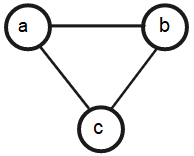
\includegraphics[width=2.3cm]{./img/trianguloabc.png} && 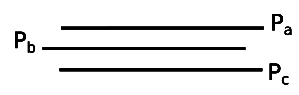
\includegraphics[width=4cm]{./img/edge-clique.png} & &
    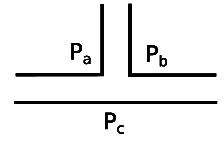
\includegraphics[width=3.3cm]{./img/claw-clique.png}
    \\
    \footnotesize %\centering 
    (a) O grafo $C_3$ && \footnotesize(b) Representação $B_0$-EPG de $C_3$ && \footnotesize (c) Representação $B_1$-EPG de $C_3$\\

  \end{tabular}

 \caption{O grafo $ C_3 $ com duas representações, uma sem dobra e outra com uma dobra} \label{fig:trianguloepgRepresentacao}
\end{figure}


%A  collection $C$ of sets satisfies the Helly property when every sub-collection of $ C $ that is pairwise intersecting has at least one common element. The Helly property has this name in honor of the great Austrian mathematician Eduard Helly, who in 1923 proposed his famous theorem concerning the relation of intersecting sets.

%The study of the Helly property is useful in very diverse areas of science, and we can enumerate applications in semantics, code theory, computational biology, database, image processing, graph theory, optimization, and linear programming \cite{dourado2009}.

%Note that the representation of Figure~\ref{fig:trianguloepgRepresentacao}(b) satisfies the Helly property, while the representations of Figures~\ref{fig:trianguloepgRepresentacao}(c) and~\ref{fig:trianguloepgRepresentacao}(d) do not satisfy it.

Este trabalho propõe o estudo de grafos que possuem uma representação EPG-Helly. 
A propriedade Helly relacionada com representações EPG foi  estudada em~\cite{golumbic2009} e \cite{golumbic2013}. Em particular, esses trabalhos determinaram um parâmetro conhecido como número de Helly forte  para grafos $B_1$-EPG. 

Estão no escopo de interesse deste trabalho os seguintes tópicos:

\begin{itemize}
    
    \item Determinar a complexidade de reconhecimento de grafos $B_1$-EPG-Helly;
    \item Determinar limites superiores e/ou inferiores para os parâmetros número de Helly e número de Helly forte em grafos EPG e EPG-Helly;
    
    \item Estudar os parâmetros número de Helly e número de Helly forte também em grafos de intersecção de vértices em caminhos sobre grade (VPG e VPG-Helly);
    
    \item Estudar o relacionamento entre as classes de grafos EPT, VPT e $B_1$-EPG.
    
\end{itemize}



% \section{Motivação}
% Por que pesquisar?

% Qual a relevância do problema e por que escolher esse tema?

% Qual é o problema estudado?
% Onde ele acontece?
% Quem observou ou observa sua ocorrência?
% Por que isso é importante e deve ser solucionado?

% \section{Objetivo}

% Quais as finalidades intelectuais?

% verificar... compreender... analizar...
% comparar...

\section{Organization of the thesis}

No Capítulo 2 apresentaremos algumas definições básicas sobre grafos juntamente com uma breve explicação sobre a propriedade Helly. Além disso, o capítulo aborda uma breve discussão sobre problemas de caminhos em grade.

O Capítulo 3 será dedicado à definição do problema estudado, análise de algumas representações EPG básicas e demonstração da $NP$-completude do problema de reconhecimento de grafos $B_1$-EPG-Helly. São publicações resultantes desta pesquisa, os seguintes escritos:

\begin{enumerate}
    \item BORNSTEIN, C. F.; SANTOS, T. D.; SOUZA, U. S.; SZWARCFITER, J. L. A Complexidade do Reconhecimento de Grafos B1-EPG-Helly. In: 50º SBPO - Simpósio Brasileiro de Pesquisa Operacional, 2018, Rio de Janeiro. Cidades Inteligentes: Planejamento Urbano, Fontes Renováveis e Distribuição de Recursos, 2018.

     \item BORNSTEIN, C. F.; SANTOS, T. D.; SOUZA, U. S.; SZWARCFITER, J. L. Sobre a Dificuldade de Reconhecimento de Grafos B1-EPG-Helly. In: XXXVIII Congresso da Sociedade Brasileira de Computação, 2018, Natal - RN. Computação e Sustentabilidade, 2018. p. 113-116.

     
     \item BORNSTEIN, C. F.; SANTOS, T. D.; SOUZA, U. S.; SZWARCFITER, J. L. The complexity of B1-EPG-Helly graph recognition. In: VIII Latin American Workshop On Cliques in Graphs (LAWCG), ICM 2018 Satellite Event, 2018, Rio de Janeiro. Program and Abstracts, 2018. p. 69.

     
     \item BORNSTEIN, C. F.; GOLUMBIC, M.C.; SANTOS, T. D.; SOUZA, U. S.; SZWARCFITER, J. L.  The complexity of B1-EPG-Helly graph recognition. %In:  45th International Workshop on Graph-Theoretic Concepts in Computer Science,  2019, Vall de Núria, Catalonia, Spain. 
     (Submited).
     
\end{enumerate}


Por fim, no Capítulo 4, discutimos os principais resultados obtidos para grafos EPG. Adicionalmente, teremos
também as considerações finais sobre o trabalho aqui apresentado com algumas perspectivas e ideias sobre o problema e possíveis direcionamentos para novos estudos de trabalhos futuros.
  \chapter{Intersection graphs of paths on grid and trees}\label{Notions}

\vspace{2.5cm}
\begin{flushright}
\begin{minipage}[t][0cm][b]{0.47\textwidth}
\emph{%Se você conhece o inimigo e conhece a si mesmo, não precisa temer o resultado de cem batalhas. 
If you know the enemy and know yourself, you need not fear the result of a hundred battles. If you know yourself but not the enemy, for every victory gained you will also suffer a defeat. If you know neither the enemy nor yourself, you will succumb in every battle.
}
\end{minipage}

\rule[0cm]{7cm}{0.03cm}%{largura}{espessura}

Sun Tzu, The Art of War
\end{flushright}

\begin{quotation}
In this chapter, we will present some concepts that will facilitate the understanding of the studied problems. In particular, we describe the notations and we will illustrate with examples only those concepts and definitions that are outside the basic scope of graph theory. As a basic bibliography on graphs, algorithms, and NP-completeness we suggest reading~\cite{bondy1976graph} and~\cite{jayme2018} .
\end{quotation}
%\section{Preliminaries}

In this thesis, we will consider finite graphs, connected and simple, i.e. graphs without loops (edge connecting a vertex in itself) or more than one edge connecting two vertices. Thus, when we talk about graphs we will consider a simple, finite and connected graph unless something different is explicitly said.

Next, we describe the terminology and notation used in this work.

A \emph{graph} $ G $ is a structure composed of two finite sets: $ V(G) $ is a non-empty set whose elements are called \emph{vertices}, and $ E(G) $ is a set of unordered pairs of distinct elements taken from $ V(G) $, which are called \emph{edges}. An edge $ e=(u, v) \in E (G) $ is formed by the pair of vertices $ u, v \in V(G) $, in this case $ u $ and $ v $ are said to be vertices \emph{adjacent}. We also say that $ e $ is \emph{incident edge} to $ u $ and $ v $. We denote the \emph{cardinality} of $ |V(G)| = n $ and $ |E(G)| = m $.

Given a vertex $v\in V(G)$,  $N(v)$ and $N[v]$ represent the \emph{open} and the  \emph{close neighborhood} of $v$ in $G$, respectively. 
For a subset $S \subseteq V(G)$,  $G[S]$ is the subgraph of $G$ induced by $S$.
 If $\mathcal{F}$ is any family of graphs, we say that  $G$ is  \emph{$\mathcal{F}$-free} if $G$ has no induced subgraph isomorphic to a member of $\mathcal{F}$.


Let $u, v$  be vertices of $G$, if $N(u) = N(v)$ then $u$ and $v$ are said \emph{false twins}, on the other hand, if $N[u] = N[v]$, then $u$ and $v$ are said \emph{true twins}. The \emph{degree of a  vertex} $v$ is denoted  by $d(v)$ and corresponds to the number of vertices adjacent to $v$, i.e., the cardinality of $|N(v)|$. The \emph{maximum degree} of a graph $G$ is denoted by $\Delta(G) = \max\{d(v) \mid v \in V(G)\}$. Similarly, the  \emph{minimum degree} is denoted by  $\delta(G) = \min \{d(v) \mid v \in V(G)\}$.

Given a graph $G$, and a vertex $v \in V(G)$, the graph $G\backslash \{v\}$ is obtained from $G$ by removing the vertex $v$ from its vertex set, and also removing all edges of $E(G)$ incidents at $v$. Similarly, given an edge $e \in E(G)$, the graph $G\backslash \{e\}$ is obtained from $G$ removing the edge $e$ from $E(G)$.

We say that $G'=(V',E')$ is a \emph{subgraph} of a graph $G=(V,E)$ when $V'\subseteq V$ and $E'\subseteq E$. When the subgraph $G'$ contains all edges of $E$ whose ends are contained in $V'$, then  $G'$ is the \emph{induced subgraph} of $G$ by $V'$.  

A graph  $G$ is a \emph{cycle}, denoted by $C_n$, if it is a sequence of vertices   $v_1, \dots, v_n, v_1$, where $v_i \neq v_j$ for $i\neq j$ and $(v_i, v_{i+1})\in E(G)$,  such that $n\geq 3$. For a cycle $C_k$, we say that it is an
\emph{even cycle} if $k$ is even and an \emph{odd cycle}, otherwise. A \emph{chord} is an edge that is between two non-consecutive vertices in a sequence of vertices of a cycle. An \emph{induced cycle}  or \emph{chordless cycle} is a cycle that has no chord. A graph that has no cycles is called \emph{acyclic}. A  graph $ G $ is \emph{connected} if there is a path between any pair of  vertices of $ G $. A graph is a \emph{tree} when it is acyclic and connected. A connected subgraph of a tree is called \emph{subtree}.

A set $\mathcal{S}$ is \emph{maximal} in relation to a particular property $P$ if $\mathcal{S}$ satisfies $P$, and each set $S'$ containing properly $\mathcal{S}$ does not satisfy $P$. In a similar way, a set $\mathcal{S}$ is \emph{minimal} in relation to a particular property $P$ if $\mathcal{S}$ satisfies $P$, and each subset  $S'$ that is properly contained in $\mathcal{S}$ does not satisfy $P$.

A graph $G$ is a \emph{intersection graph} of a family of subsets of a set $\mathcal{S}$, when it is possible to associate each vertex $v \in V(G)$ to a subset $S_v \subseteq \mathcal{S}$, such that $S_u \cap S_v \neq \emptyset$ if and only if $(u,v)\in E(G)$.  In this thesis, in particular, we will study four families of intersection graphs: the VPG, EPG, VPT and EPT graphs.


The term \emph{grid} is used to denote the Euclidean space of entire orthogonal coordinates. Each pair of entire \emph{coordinates} corresponds to a point or \emph{vertex of the grid} (which by the context is not to be confused with the vertex of the graph). The term \emph{grid edge} (which is also not to be confused with the edge of the graph), will be used to denote a pair of vertices that are at distance one in the grid. Two edges $ e_1 $ and $ e_2 $ are \emph{consecutive edges} when they share exactly one point on the grid. A grid is the \emph{host} on which we accommodate the VPG and EPG representations. When we refer to the VPT and EPT graphs, we implicitly know that the host of their representations is a tree.



 A \emph{path in the grid} is distinguished by two contexts, in the first we study families of subsets $\cal{F}$ of edge of the grid. In this context a path in the grid is defined as a finite sequence of consecutive edges  $e_1 = (v_1, v_{2}), e_2 = (v_2, v_{3}), \dots, e_i = (v_i, v_{i+1}), \dots, e_m = (v_{m}, v_{m+1})$,  where   $v_i \neq v_j$ for $i \neq j$.  We call a collection of such paths an {\it EPG representation}, i.e., a collection of paths that represent a graph via its intersection graph (considering edge intersections). {\it EPG graphs} are the class of graphs that admit an EPG representation.
  In the second context, for vertex paths, we study families of subsets $\cal{F}$ of vertex of the grid, and a path consists of a sequence of consecutive vertices of the grid  $v_1, v_2, \dots , v_k$ such that $(v_i, v_{i+1})$ is an edge of the grid, for all $i \in {1, \dots,  k - 1}$, where   $v_i \neq v_j$ for $i \neq j$, and a collection of these paths forms a {\it VPG representation} and corresponds to a {\it VPG graph}. 

 
 The first and last edges of a path are called \emph{extremities edges}.
The \emph{direction of an edge} is \emph{vertical} when the first coordinate of its vertices is equal, and is \emph{horizontal} when the second coordinate is equal. A \emph {bend} in a path is a pair of consecutive edges $ e_1, e_2 $ of the path, such that the directions of $ e_1 $ and $ e_2 $ are different. When two edges $ e_1 $ and $ e_2 $ form a bend, they are called \emph{bend edges}. A \emph{segment} is a path without bend.
 
 In context of EPG graphs, we say that two paths are
 \emph{edge-intersecting}, or simply  \emph{intersecting}, if these share at least one edge (of the grid).
 
 
 EPG graphs are a class of  intersection graphs of paths on a grid~\cite{golumbic2009}. Shortly after came the VPG graphs, this class was introduced in 2011 \cite{asinowski2011string} and \cite{asinowski2012}. 
 These classes consist of graphs whose vertices can be represented by paths of a grid $ Q$, such that two vertices of $ G $ are adjacent if and only if the corresponding paths intersect (in edges, if EPG graphs or in vertex, if VPG graphs). If every path in a representation can be represented with a maximum of $ k $ bends, we say that this graph $ G $ has a  \emph{$ B_k$-EPG} (resp. \emph{$ B_k$-VPG}) representation. When $ k = 1 $ we say that this is a \emph{single bend} representation.

 Let $P$ be a family of paths on a host tree $T$ . Two types of intersection graphs from the pair $<P,T>$ are defined, namely VPT and EPT graphs.
The \textit{edge intersection graph} of $P$, EPT(P), has vertices which correspond to the members of $P$, and two vertices are adjacent in EPT(P) if and only if the corresponding paths in $P$ share at least one edge in T. Similarly, the \textit{vertex intersection graph} of $P$, VPT(P), has vertices which correspond to the members of $P$, and two vertices are adjacent in VPT(P) if and only if the corresponding paths in $P$ share at least one vertex in $T$.
%
VPT and EPT graphs are incomparable families of graphs. However, when the maximum degree of the host tree is restricted to three the family of VPT graphs coincides with the family of EPT graphs \cite{golumbic1985edge}. Also, it is known that any Chordal EPT graph is VPT (see~\cite{syslo1985triangulated}). Recall that it was shown that Chordal graphs are the vertex intersection graphs of subtrees of a tree \cite{gavril1974intersection}.
% \cite{alcon2010necessary

We say that a family  $\mathcal{F}$ of sets is \emph{$k$-intersecting} if for each $F_1, F_2, \dots, F_k$ subsets of $\mathcal{F}$, we have that $F_1\cap F_2 \cap \dots \cap F_k \neq \emptyset$. We also say that a family $\mathcal{F}$  of sets is \emph{$k$-Helly}, when every subfamily $k$-intersecting $F'$ of  $\mathcal{F}$ has at least one common element.
 In particular, we say that a family of sets is \emph{pairwise intersecting}, i.e. two by two intersecting if any two sets in the family intersect. A collection $ C $ of non-empty sets satisfies the Helly property, i.e. it is $ 2$-Helly, when every subcollection pairwise intersecting $ S $  of $ C $ has at least one element that is in every subset of $ S$.

For simplicity of notation, in this thesis when we refer to a family of sets as a Helly family it is understood that this family is $ 2$-Helly.

In Boolean algebra, a \emph{clause} is a disjunction or conjunction of literals. We say that a \emph{formula} $ F $ is in the \emph{Conjunctive Normal Form} (CNF) if $ F $ is a conjunction of clauses, where a clause is a disjunction of literals.

\section{Related Works}

In this section, we will present the main known results on the related study topics in this work, namely Helly property, EPG, VPG, EPT, and VPT graphs.

\subsection{On the Helly property}


The Helly property is named in honor of the Austrian mathematician Eduard Helly, who in 1923 proposed a famous theorem about the relationship of intersecting sets. Such a theorem motivates the so-called \textit{Helly property} which can be  stated as follows: given a collection of  sets $ C$, not empty, we say that this collection satisfies the Helly property when every subcollection of $C$ that is pairwise intersecting has at least one element in common.


We can note that the Helly property is a topic that has instigated scientific research since it appeared, moreover, we can also mention recent works in the area of Graph Theory, see~\cite{berge1973, bergeDuchet1975, DOURADO2008, golumbic2013, dourado2006computational, teles2016, jose2018}.
The study of the Helly property proves to be useful in the most diverse areas of science, of which one can enumerate applications in semantics, code theory, computational biology, database, image processing, graph theory, optimization, in problems of location and linear programming, \cite{teles2016}. In particular, in the area of Graph Theory, the Helly property has motivated the study of several graph classes, for example, we can cite the  Clique-Helly graphs~\cite{DOURADO2008}, Helly Circular-arc~\cite{safe2016essential}, Helly EPT~\cite{alcon2017helly}, Disk-Helly~\cite{lin2007faster} and Helly Hypergraphs~\cite{mulder1979median}.


In addition to the applications mentioned above, the Helly property can be studied on  $ B_k$-EPG representations, where each path is considered as a set of edges. A  graph $ G $ has a Helly-$B_k$-EPG representation if there is a $ B_k$-EPG representation of $ G $ where each path has at most $ k $ bends and the representation satisfies the Helly property.
We will use the  notation $ P_{v_i} $ to indicate the path corresponding to the  vertex $ v_i$.
Figure~\ref{fig:envelopeRepresentacoes}(a) depicts two representations $ B_1$-EPG of a graph with 5 vertices. Figure~\ref{fig:envelopeRepresentacoes}(b) depicts pairwise intersecting paths ($ P_{v_1}, P_{v_2}, P_{v_5} $), containing a common edge, so this is a  Helly-$B_1$-EPG representation. In Figure~\ref{fig:envelopeRepresentacoes}(c), although the 3 paths are pairwise intersecting, there is no edge common to the 3 paths simultaneously, and thus they do not satisfy the Helly property.


\begin{figure}[h]
  \centering
  \begin{tabular}{ p{3.2cm} p{4.5cm} p{4.5cm} }
    \centering 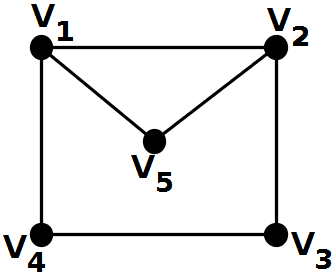
\includegraphics[width=3cm]{./img/envelope} & 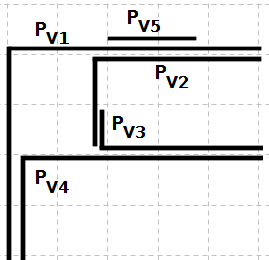
\includegraphics[width=4cm]{./img/envelopeHellyGradeTransparente} & 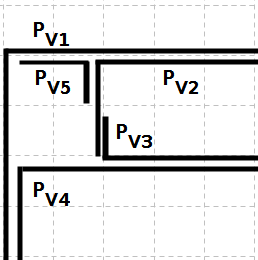
\includegraphics[width=4cm]{./img/envelopeNaoHellyGrade}
    \\
    \footnotesize \centering (a) A  graph with 5 vertices. & \footnotesize(b) A $B_1$-EPG representation that satisfies the Helly property. & \footnotesize (c) A $B_1$-EPG representation that does  not satisfy the Helly property.  \\

  \end{tabular}
\caption{A  graph with 5 vertices in (a) and some single bend representations: Helly in (b) and not Helly in (c).} \label{fig:envelopeRepresentacoes}
\end{figure}

%%%%%%%%%%%%%%%%%%%%%%%%%%%%%%%%%%%%%%%%%%%%%%%%%%%%%%%%%%%%%

In this thesis, we are interested in EPG representations of graphs that satisfy the Helly property. In particular, for the $ B_1$-EPG graphs, this directly implies that each clique has a special format, and the paths that compose it always share an edge of the representation in the grid, i.e. an edge-clique. Using this premise we were able to present Helly subfamilies for $ B_1$-EPG graphs and we also presented a hardness proof  in recognizing this class of graphs.
 We will also study within the scope of this research the parameters Helly number and strong Helly number in paths on a grid.

\subsection{On EPG graphs}

A problem related to the study of EPG graphs is the problem of edge-intersection graphs of paths in a tree, well known in the literature as EPT (Edge-intersection Graphs of Paths in a Tree), see for instance~\cite{gavril1974intersection, golumbic2004recognition}. For EPT graphs, in particular, the value of the parameters Helly number, which is 2, and the strong Helly  number, which is 3, are known results, also in~\cite{golumbic2004recognition}. The parameters Helly number and strong Helly number had been studied in EPT graphs when the set of paths satisfies the Helly property, see
~\cite{petito2002grafos} and \cite{petito2009grafos}.

Regarding the complexity of the $B_k$-EPG graph recognition, only the hardness recognition of a few of these graph subclasses was determined.  $ B_0$-EPG can be recognized in polynomial time, since these correspond to the interval graphs, see~\cite{booth1976}. In contrast, the $ B_1$-EPG and $ B_2$-EPG graphs recognition are $ NP$-complete problems, see~\cite{heldt2014, martin2017}, and the $ B_1$-EPG graph recognition problem remains $ NP$-complete even  for $ L$-shaped paths on a grid, see~\cite{cameron2016edge}. Moreover, in this doctoral thesis you will also find an $ NP$-completeness proof  for the  Helly-$B_1$-EPG graphs recognition in Chapter~\ref{cap:capiii}, and the same chapter we further studied the subsets of $L$-shapes and its relationship with $B_1$-EPG and Helly-$B_1$-EPG graphs.

In this work, we are going to study graphs that have a Helly-EPG representation and related subjects.  The Helly property related to EPG graph representations was studied by~\cite{golumbic2009} and~\cite{golumbic2013}. In particular, they determined the parameter strong Helly number of graphs $ B_1$-EPG. We determine two parameters to every class of EPG graphs, the Helly number and strong Helly number, these results are presents in Chapter~\ref{cap:iv}.

Research about graphs of edge-intersection of  paths on a grid is a relatively new topic in the area of Graph Theory. The first formal definitions of problems and applications were presented by Golumbic in 2009~\cite{golumbic2009}. Since then, several branches of researches have been conducted by the scientific community. These questions often discuss the path representations, restrictions on the bend number in a representation, among others. 
A survey that summarizes the state-of-the-art for the topic of EPG graphs can be found at~\cite{chung201950}. 

Next, we present  some results regarding the  \emph{bend number} for some classes of graphs, among others.

In their study, \citeauthor{alcon2016}~\cite{alcon2016}, the authors show that 3 bends are enough to represent all graphs in the class of circular-arc graphs, i.e. they are in $ B_3$-EPG. Additionally, they also show that there are circular-arc graphs that cannot be represented with 2 bends. Using the fact that we can to represent any circular-arc graph using only a rectangle of a grid of any size, the work defines the class of EPR graphs and classifies the normal circular-arc graphs  as being $ B_2$-EPR, they also show that there are normal circular-arc graphs that are not $ B_1$-EPR. Finally, the work gives a characterization of $ B_1$-EPR graphs by a minimal family of forbidden induced subgraphs and shows that this subfamily corresponds to a subclass of normal Helly Circular-arc graphs.


In the paper of ~\citeauthor{biedl2010}~\cite{biedl2010}, the authors show that 5 bends are enough to represent all planar graphs and that 3 bends are enough to represent all outerplanar graphs. These results are further improved by~\cite{daniel2014b}. In addition to these results, the work shows that every Bipartite Planar graph has a $B_2$-EPG representation and that every Line graph has a $B_2$-EPG representation. In this thesis, we demonstrate that every Line of Bipartite graph is in Helly-$B_1$ EPG, these results are in Chapter~\ref{cap:v}.

\citeauthor{daniel2014b} in~\cite{daniel2014b} showed that 4 bends are enough to represent all planar graphs and present a linear algorithm to find this representation with 4 bends. However, the authors still comment that for some planar graphs, 3 bends are often enough to construct the representation. In fact, it is not that simple the majority of planar graphs could be constructed with 4 bends, in fact, there are no known planar graphs that cannot be drawn using 3 bends. This leaves the question: if 4 bends are always enough to represent any planar graph, then are 4 bends really needed to represent any planar graph? That question is still open. The authors still conjecture that there is a graph where for any of its EPG representations there is always at least one path that needs to use the 4 bends.


The Table~\ref{tab:limitesBenNumber} presents the main known bounds for the \emph{bend number}, denoted by $b(G)$, of some graph classes.


\begin{table}[h]
\caption{Some graph classes and  known bounds to their \textit{bend number}.}
\label{tab:limitesBenNumber}
\begin{center}
\begin{tabular}{|c|c|c|}
\hline 
Graph Class & b(G) & Reference \\ 
\hline \hline  
Interval graphs & 0 & \cite{golumbic2009} \\ 
\hline 
Forests, Cycles & 1 & \cite{golumbic2013} \\ 
\hline 
Outerplanar &  2 & \cite{daniel2014b} \\ 
% \hline 
% Planar & 5 e dim $(n-1)\times(2n-3)$ & \cite{biedl2010} 2010\\ 
\hline 
Planar & $\in [3, 4]$ & \cite{daniel2014b}\\ 
\hline  
  Bipartite Planar & 2 & \cite{biedl2010} \\ 
\hline 
Line Graph & 2 & \cite{biedl2010} \\ 
\hline 
dgn(G)~\footnotemark %\footnote{Degeneracy}
$\leq k$ & $2k-1$ & \cite{daniel2014b} \\ 
\hline 
tw(G)~\footnotemark%\footnote{Treewidth} 
$\leq k$ & $2k-2$ & \cite{daniel2014b} \\ 
\hline 
Degree $\leq \Delta$ & $ \in [	\lceil \frac{\Delta}{2}\rceil, \Delta ] $ & \cite{daniel2014b} \\ 
\hline 
Circular-arc & 3 & \cite{alcon2016} \\ 
\hline 
Normal Circular-arc & 2 & \cite{alcon2016} \\ 
\hline 
Halin graphs & 2 & \cite{mathew2016}  \\ 
\hline 
\end{tabular} 
\end{center}
\end{table}



\footnotetext[1]{Degeneracy}
\footnotetext[2]{Treewidth}
% \footnotetext{Degeneracy}
% \footnotetext{Treewidth}

In addition to the results cited for bounds on the bend number of some classes of graphs, there are many works that characterize other types of graphs not mentioned in this table, such that the work of~\citeauthor{ries2009} in~\citep{ries2009} that characterizes the Chordal graphs  claw-free, bull-free and diamond-fee that have a $ B_{1}$-EPG representation. In that same article, there is also a characterization of some Split graphs, with a restriction on the size of the independent set or  clique, by forbidden subgraphs. The work still has an interesting result that shows that the neighborhood of every vertex of a graph $ B_1$-EPG induces a graph that is Weakly Chordal. Implicitly this paper delimits a set of Helly-$B_1$-EPG graphs, the bull-free graphs. Based on this fact in this thesis, we extend the results to delimit another Helly-$B_1$-EPG subfamily, the diamond-free subfamily. This result can be found in Chapter~\ref{cap:v}.

Although it is possible to find several lines of researches on EPG graphs investigating the bend number, the interests of studies in this class of graphs extend to other classic problems, which we can mention to follow.


In~\citet{cohen2014} a linear time recognition algorithm is presented for $ B_{1}$-EPG Cographs by a family of forbidden induced subgraphs. The algorithm that the paper presents uses the Cotree of the Cograph in the recognition process.

Approximation Algorithms for colorize $ B_1$-EPG graphs  were studied in~\cite{epstein2013approximation}. The work cited shows that the coloring problem and the maximum independent set problem are both $ NP$-complete for graphs $ B_1$-EPG even when the EPG representation is given. The authors present a 4-approximate algorithm that solves both problems, assuming that the EPG representation is given. The work still shows that the maximum clique can be found efficiently in graphs $ B_1$-EPG even when the representation is not given.

Clique coloring problems in $B_1$-EPG graphs were studied by~\cite{bonomo2017clique}. The authors consider the clique coloring problem and show that $B_1$-EPG graphs are 4-clique-colorables and present a linear time algorithm to solve the problem. Moreover, given a $B_1$-EPG representation of a graph, the paper provides a linear time algorithm that constructs a 4-clique coloring of it.
 
We can also mention as an often research with respect to EPG graphs the study of $NP$-hardness~\cite{daniel2014b, martin2017}, area of the grid necessary to represent a graph whose maximum degree is $\Delta(G)$~\cite{Asinowski2009}, and many others. The hardness of recognizing few classes of EPG graphs is known, and even for small $ k $ values only. Research with EPG graphs whose representations satisfy the Helly property is sparse. Thus, these topics and other similar topics prove to be interesting branches of research from a scientific point of view.

Finally, we mention that the $B_k$-EPG hierarchy is proper, i.e.,

$B_0$-EPG $\subset$ $B_1$-EPG $\subset$ $B_2$-EPG $\subset \dots$ $B_{k-1}$-EPG $\subset$ $B_k$-EPG $\subset$ $B_{k+1}$-EPG 

this result is demonstrated by~\citet{biedl2010} for even $k$ and  \citet{heldt2014} complete the result for all $k$.
A correlated result is presented by~\citet{Asinowski2009} that proved that for any $k$, only a small fraction of all labeled graphs on $n$ vertices are $B_k$-EPG.

\subsection{On VPG graphs}

VPG representations arise naturally when studying circuit layout problems
and layout optimization where layouts are modeled as paths (wires) on
grids. One approach to minimize the cost or difficulty of production involves minimizing the number of times that each path bend, see~\cite{bandy1990, molitor1991, sinden1966topology}.
Other times layout may consist of
several layers where the paths on each layer are not allowed to intersect. This is naturally modeled as the coloring problem on the corresponding intersection graph, see~\cite{Alcn2017VertexIG}.


A graph is a VPG if it is the vertex intersection graph of paths in a grid. A graph is called
$B_k$-VPG if it has a $B_k$-VPG representation, i.e. if there is a representation where each path in this representation has at most $k$ bends. VPG graphs were introduced in 2011 by~\citet{asinowski2011string} and~\citet{asinowski2012}. They prove that VPG and String are
the same graph class. However, it is known that  recognizing String graphs is an $NP$-complete problem, by the results of~\cite{schaefer2003recognizing, kratochvil1991string}.

\citet{asinowski2012} study $B_0$-VPG graphs and observe
that horizontal and vertical segments have strong Helly number 2 and that the clique problem has polynomial-time complexity, given the path representation. Among other results, they present proof that the recognition and coloring problems for $B_0$-VPG graphs are $NP$-complete. Moreover, they  give a 2-approximation algorithm for coloring $B_0$-VPG graphs. Furthermore, they prove that triangle-free $B_0$-VPG graphs are 4-colorable, and this is best  possible. In addition, they present a hierarchy of VPG graphs relating them to other known families of graphs, see Figure~\ref{fig:hierarquiaVPG}. The grid intersection graphs are shown to be equivalent to the bipartite $B_0$-VPG graphs and the circle graphs are strictly contained in $B_1$-VPG. They still prove the strict containment of $B_0$-VPG into $B_1$-VPG, and conjecture that, in general, this strict containment continues for all values of $k$. Finally, they present
a graph that is not in $B_1$-VPG. 

\begin{figure}[htb]	
\center%6.3
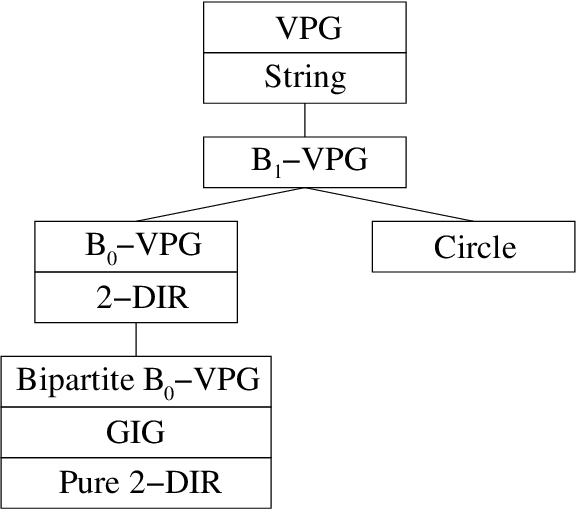
\includegraphics[width=6cm]{./img/hierarquiaVPG.png}
\caption{Relations between $B_k$-VPG graphs and well known graph classes \cite{asinowski2012}. }
\label{fig:hierarquiaVPG}
\end{figure}


It is known that all planar graphs are $B_2$-VPG, see~\cite{chaplick2012planar}. This paper also shows that the 4-connected planar graphs constitute a subclass
of the intersection graphs of $Z$-shapes (i.e., a special case of $B_2$-VPG). Additionally, they demonstrate that a $B_2$-VPG representation of a planar
graph can be constructed in polynomial time. They further show that the triangle-free planar graphs are contact graphs of L-shapes, $\Gamma$-shapes, vertical segments, and horizontal segments (i.e., a special case of contact $B_1$-VPG). 

Approximation algorithms for the maximum independent set problem over the class of $B_1$-VPG graphs are presented by~\citet{lahiri2015maximum}. Also, the NP-completeness of the decision version restricted to unit length equilateral   $B_1$-VPG graphs was established by them.

\citet{cohen2016posets} investigate the VPG graphs, and specifically the relationship between the bend number of a Cocomparability graph and the poset dimension of its complement. They show that the bend number of a Cocomparability graph $G$ is at most the poset dimension of the complement of $G$ minus one. Then, via Ramsey type arguments, they show that their upper bound is best  possible.


In \citet{felsner2016intersection}, the authors research the L-shapes representations for $B_k$-VPG graphs. The paper investigates several known subclasses of segment graphs (SEG-graphs), motivated mainly by research \cite{middendorf1992max} that states that every $[\llcorner, \ulcorner]$-shape is an SEG-graph.
They show that these subclasses of SEG-graphs belong to $[\llcorner]$-shapes, also that all Planar 3-trees, all Line graphs of Planar graphs, and all full subdivisions of Planar graphs are $[\llcorner]$-shapes. Furthermore,  \citet{felsner2016intersection} showed that the complement of Planar graphs is $B_{17}$-VPG graphs and complements of  full subdivisions of the latter class are $B_2$-VPG graphs. 

In the paper of \citet{golumbic2013intersection} certain subclasses of $B_0$-VPG graphs have been characterized and showed to admit polynomial-time recognition. We can list these classes as Split, Chordal claw-free, and Chordal bull-free $B_0$-VPG graphs.
The $B_0$-VPG Split graphs were characterized by  a set of forbidden induced subgraphs. %The same is true for another listed subclasses.


In \citet{chaplick2011recognizing}, they investigate  $B_0$-VPG graphs. Their paper describes a polynomial time
algorithms for recognizing chordal $B_0$-VPG graphs, and for recognizing $B_0$-VPG graphs that have a representation on a grid with 2 rows and an arbitrary number of columns.

\citet{chaplick2012bend} show  that for every fixed $k$, $B_k$-VPG $\subsetneq$ $B_{k+1}$-VPG and that recognition of graphs from $B_k$-VPG is $NP$-complete even when the input graph is given by a $B_{k+1}$-VPG representation. 


$B_0$-VPG graphs restricted to Block graphs were studied by \citet{Alcn2017VertexIG}. Their research has given a characterization by an infinite family of minimal forbidden induced subgraph  for $B_0$-VPG Block graphs. Furthermore, the work provides an alternative recognition and representation algorithm for $B_0$-VPG graphs also in the class of Block graphs.

In Chapter~\ref{cap:iv} we study the parameters Helly number  and strong Helly number for $B_k$-VPG graphs. We determine the value of these parameters to $ k = 0,1,2,3 $ and verify that they are unbounded for $ k\geq 4 $.



\subsection{On EPT and VPT graphs}

Models based on paths intersection  may consider  intersections by vertices or   intersections by edges.  Cases where the paths are hosted on a tree  appear first in the literature, see for instance \cite{gavril1978recognition, golumbic1985edge, golumbic1985}.  Representations using paths on a grid were considered later, see  \cite{golumbic2009,golumbic2013, golumbic2013intersection}.

EPT and VPT graphs have applications in communication networks, see~\cite{boyaci2013graphs} in~\cite{brandstadt2013graph}. Assume
that we model a communication network as a tree $T$ and the message routes to be delivered in this communication network as paths on $T$. Two paths conflict if they both require to use the same link (vertex). This conflict model is equivalent to an EPT (a VPT) graph. Suppose we try to find a schedule for the messages such that no two messages sharing a link (vertex) are scheduled in the same time interval. Then a vertex coloring of the EPT (VPT) graph corresponds to a feasible schedule on this network, ~\cite{boyaci2013graphs} and~\cite{brandstadt2013graph}.

 Let $P$ be a family of paths on a host tree $T$. Two types of intersection graphs from the pair <$P,T$> are defined, namely VPT and EPT graphs.
The \textit{edge intersection graph} of $P$, EPT(P), has vertices which correspond to the members of $P$, and two vertices are adjacent in EPT(P) if and only if the corresponding paths in $P$ share at least one edge in T. Similarly, the \textit{vertex intersection graph} of $P$, VPT(P), has vertices which correspond to the members of $P$, and two vertices are adjacent in VPT(P) if and only if the corresponding paths in $P$ share at least one vertex in $T$.

VPT and EPT graphs are incomparable families of graphs. However, when the maximum degree of the host tree is restricted to three the family of
VPT graphs coincide with the family of EPT graphs \cite{golumbic1985edge}. Also, it is known that any Chordal EPT graph is VPT, see~\cite{syslo1985triangulated}. Recall that it was shown that Chordal graphs are the vertex intersection graphs of subtrees of a tree \cite{gavril1974intersection}.

Next, we list some research involving EPT and VPT graphs.

%EPT and VPT graphs have been extensively studied in the literature. 
Although VPT graphs can be characterized by a fixed number of forbidden subgraphs, see~\cite{leveque2009characterizing}, it is shown that EPT graphs recognition is an NP-complete problem, see~\cite{golumbic1985}. Main optimization and decision problems such as recognition~\cite{gavril1978recognition}, the maximum clique~\cite{gavril2000maximum} , the minimum vertex coloring~\cite{golumbic2004algorithmic}  and the maximum stable set problems~\cite{spinrad1995algorithms} are polynomial-time solvable in VPT whereas recognition and minimum vertex coloring problems remain NP-complete in EPT graphs~\cite{golumbic1985edge}. In contrast, we can solve in polynomial time the maximum clique,
see~\cite{golumbic1985}, and the maximum stable set, see~\cite{tarjan1985decomposition},  problems in EPT graphs. 

In~\citet{alcon2010necessary} we find a short paper that deals with EPT graphs. The paper defines the concept of satellite of a clique and we give us a necessary condition for the  structure of cliques in EPT graphs based on satellites of cliques. In addition, the paper presents a finite family of minimal forbidden subgraphs for the EPT class.

Next, we will present the notation $[h,s,t]$ so that we can talk about some equivalences known in the literature.


The class of graphs that have an $[h,s,t]$-representation is denoted by $[h,s,t]$. A graph $G$ has an $[h,s,t]$-representation  when $h,s,$ and $t$ are positive integers such that $h \geq s$, there is a host tree $T$ with maximum degree $\Delta(T) \leq h$, there is a family of subtrees $S = \{S_u \subseteq T / u\in V(G) \}$ with $\Delta(S_u)\leq s$, and there is an edge $uv \in E(G)$ if and only if $|S_u \cap S_v|\geq t$.    

In~\citet{alcon2015characterizing} was studied a set of minimal forbidden induced subgraphs from VPT and their $[h,s,t]$-representations.
When there is no restriction on the maximum degree of $T$ or on the maximum degree of the subtrees is used the notation $h=\infty $  and $s=\infty$,  respectively. Therefore, $[\infty, \infty, 1]$ is the class of Chordal graphs and $[2, 2, 1]$ is the class of interval graphs. The classes $[\infty, 2, 1]$ and $[\infty, 2, 2]$ correspond to VPT and EPT respectively in~\cite{golumbic1985edge}; and UV and UE, respectively in~\cite{monma1986intersection}.
By taking $h=3$ they obtain a characterization by minimal forbidden induced subgraphs of the class VPT $\cap$ EPT = EPT $\cap$ Chordal = $[3,2,2] = [3,2,1]$, see~\citet{golumbic1985edge}. The paper also proved that the problem of deciding whether a given VPT graph belongs to $[h,2,1]$ is NP-complete even when restricted to the class VPT $ \cap $ Split without dominated stable vertices, among other minor results.


Priscila Petito in her master thesis \cite{petito2002grafos} researched UE graphs, UV graphs, and the Helly property. In particular, when it considers the UE family with Helly property its study leads to a new graph class denoted by UEH graph class. The master thesis also presents results to directed and rooted trees. Furthermore, the master thesis also considers the relationship among these classes in addition to others. In time, the work still considers the parameter strong Helly number in its scope. This doctoral thesis approaches a similar branch of research since we studied EPG and Helly graphs, the parameters Helly number and Strong Helly number, and also VPT and EPT (UV and UE respectively) graphs.

 %\citet{petito2002grafos} continued her study in her doctoral thesis. 
 
 
 In Priscila Petito's doctoral thesis  \cite{petito2009grafos} UEH graphs  were studied. The work presents a characterization by forbidden subgraphs that are simultaneously UEH and Split.  Among the main problems addressed in the research are also the clique coloring problem in UEH graphs,  the study of the complexity of the sandwich problem for the Clique-Helly class. In addition, the work also studies the inclusion relations among UE, UEH, and Clique-Helly classes.

Returning to $[h,s,t]$ notation, it is known that when the EPT graphs are restricted to host trees of vertex degree 3 this class corresponds precisely to the Chordal EPT graphs. In~\citet{golumbic2008representing} was  proved an analogous result that Weakly Chordal EPT graphs are precisely the EPT graphs whose host tree restricted to degree 4. Moreover, they provide an algorithm to reduce a given EPT representation of a Weakly Chordal EPT graph to an EPT representation on a degree 4 tree. In short, their proof state that  $[4, 2, 2]$ graphs are equivalent to Weakly Chordal $[\infty, 2, 2]$ graphs. In addition, we know that when the maximum degree of the host tree T is 3, the coloring problem is polynomial, by
~\cite{golumbic1985}. The paper of~\cite{golumbic2008representing} also shows the analogous polynomial result for a degree 4 host tree, thus the coloring problem on EPT graphs restricted to a host tree of vertex degree 4 is polynomial.

In~\citet{golumbic2008equivalences}, the research presents equivalences and the complete hierarchy of intersection graphs of paths in a tree, this including VPT and EPT grpahs, in particular orthodox-$[h,s,t]$ graphs with $s=2$ and considering variations of $h,t$. For more information about orthodox-$[h,s,t]$ graphs we recommend reading~\citet{jamison2005constant} and \citet{jose2018}.

Other researches still focus on variations of the EPT representations, such as \cite{boyaci2013graphs} and \cite{boyaci2016graphs}. These two articles represent the same research divided into two parts. Given a set of paths $P$, they define the graph ENPT($P$) of edge intersecting non-splitting paths of a tree, denoted by ENPT graph, as the graph having a vertex for each path in $P$, and an edge between every pair of vertices representing two paths that are both edge-intersecting and non-splitting. A graph $G$ is an ENPT graph if there is a tree $T$ and a set of paths $P$ of $T$ such that $G$ = ENPT($P$). The papers investigate the basic properties of this class and proof that some graph classes belong to ENPT, such that Trees, Holes, Complete graphs, etc. Among the results, they show that the problem of finding such a representation is $NP$-Hard in general also for this class.

As we can see, EPT and VPT graphs have been extensively studied in the literature. With approaches that study from classic problems in these classes of graphs to variations of constructions and representations in those same classes. In this thesis, in particular, we will study the relationship of the VPT and EPT graphs with the EPG graphs.

In Chapter~\ref{cap:v} we consider relationship between classes VPT, EPT and Chordal $B_1$-EPG graphs.

In the next section, we present a table with the main notations used in the text.

%\subsection{The VPT graphs}

\section{Terminology}

Table~\ref{tab:terminologyTable} describes the basic symbols and their meanings about graph theory.
More specific definitions will be given in the next chapters as necessary.

\rowcolors{2}{gray!25}{white}
\begin{table}[h]
\caption{Terms and basic symbols of Graph Theory used in this thesis.}
\label{tab:terminologyTable}
\begin{center}
\begin{tabular}{|c|p{10cm}|}
 \rowcolor{gray!50}
\hline 
Symbol & Description \\ 
\hline \hline  
$G=(V,E)$& Graph $G$ with vertex set $V(G)$ and edge set $E(G)$. \\
\hline 
$V(G)$ & Vertex set of $G$. \\
\hline 
$E(G)$ & Edge set of $G$.\\
\hline 
$n(G)$& Number of vertices in $G$. \\
\hline 
$m(G)$& Number of edges in $G$.\\
\hline 
$v_i$& Vertex $v_i$. \\
\hline 
$P_{v_i}$& Path corresponding to the vertex $v_i$. \\
\hline 
$e=(v_i,v_j)$& Edge $e$ with endpoints  $v_i$ and $v_j$. \\
\hline 
$d(v)$& Degree of vertex $v$. \\
\hline 
$\delta(G)$& Minimum degree of a vertex in $G$. \\
\hline 
$\Delta(G)$ & Maximum degree of a vertex in $G$.  \\
\hline 
$N(v)$ & Opened neighborhood of the vertex $v$. \\
\hline 
$N[v]$& Closed neighborhood of the vertex $v$. \\
\hline 
$G[S]$ & Induced subgraph in $G$ by subset of vertices $S$. \\
\hline 
$|S|$ & Cardinality of set $S$. \\
\hline 
$G\backslash \{v\}$ & Subgraph obtained of $G$ by removing the vertex $v$. \\
\hline 
$C_n$ & Induced Cycle with $n$ vertices. \\
\hline 
$W_n$ & Wheel graph with $n$ vertices. \\
\hline
$K_{r,s}$  &  Complete Bipartite graph with parts os size $r$ and $s$.   \\
\hline
  $K_n$ & Complete graph or clique with $n$ vertices.   \\
 \hline 
 $B_k$-representation & Representation where each path has at most $k$ bends.  \\
 \hline
  $<P,T>$ & Set of paths $P$ on a tree $T$.  \\
  $[h,s,t]$-representation & Representation on a host tree of degree at most $h$ of subtrees of degree at most $s$ and intersection of lenght at least $t$.  \\
\hline 
\end{tabular} 
\end{center}
\end{table}

\rowcolors{2}{white}{white}


In the following chapters, we will dedicate ourselves to expose the main results obtained by researching this thesis.
  \chapter{The Helly property and EPG graphs}\label{cap:capiii}

\begin{flushright}
\begin{minipage}[t][0cm][b]{0.47\textwidth}
\emph{
Talento é 1\% inspiração e 99\% transpiração. }
\end{minipage}

\rule[0cm]{7cm}{0.03cm}%{largura}{espessura}

Thomas Edison
\end{flushright}

% Neste capítulo examinaremos as relações hierárquicas entre algumas classes EPG e EPG-Helly. Ademais, abordaremos representações $B_1$-EPG de alguns grafos que serão utilizados posteriormente. Primeiro, vamos observar como as classes $B_0$-EPG, $B_0$-EPG-Helly, $B_1$-EPG e $B_1$-EPG-Helly se relacionam, em seguida consideramos as representações $B_1$-EPG de $C_4$'s e do grafo octaedro. Por último, apresentaremos a prova de $NP$-completude do problema de reconhecimento de grafos $B_1$-EPG-Helly.

In this chapter we will examine the hierarchical relationships among some EPG and Helly-EPG classes. In addition, we will approach $ B_1$-EPG representations of some graphs that will be used later. First, let is focus our attention to understand how the classes $B_0$-EPG, $B_1$-EPG,  Helly-$B_1$ EPG and  $L$-shaped paths are related, then we consider the $ B_1$-EPG representations of graphs $C_4 $ and the Octahedral graph. Next, we will present the proof of $NP$-completeness to Helly-$B_1$-EPG graph recognition problem. Finally, at the end of this chapter the reader can find a section with a complete version of the paper published in the journal DMTCS that contains the set of proofs that have been omitted from the text.


\section{Introduction}
An EPG graph $G$ is a graph that admits a representation in which its vertices are represented by paths of a grid $Q$, such that two vertices of $G$ are adjacent if and only if the corresponding paths have at least one common edge.

The study of EPG graphs has motivation related to the problem of VLSI design that combines the notion of edge intersection graphs of paths in a  tree with a  VLSI  grid layout model, see~\cite{golumbic2009}. The number of bends in an integrated circuit may increase the layout area, and consequently, increase the cost of chip manufacturing.
This is one of the main applications that instigate research on the EPG representations of some graph families when there are constraints on the number of bends in the paths used in the representation.
Other applications and details on circuit layout problems can be found in~\cite{bandy1990, molitor1991}.

A graph is a $ B_k$-EPG graph if it admits a representation in which each path has at most $k$ bends. As an example, Figure~\ref{fig:trianguloepgRepresentacao}(a) shows a $C_3$, Figure~\ref{fig:trianguloepgRepresentacao}(b) shows an EPG representation where the paths have no bends and Figure~\ref{fig:trianguloepgRepresentacao}(c) shows a representation with at most one bend per path.   
Consequently, $C_3$ is a $B_0$-EPG graph. More generally, $B_0$-EPG graphs coincide with interval graphs.


\begin{figure}[h]
  \centering
  \begin{tabular}{ p{3cm} p{0.7cm} p{4cm} p{0.7cm} p{4cm} }
    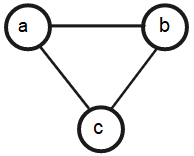
\includegraphics[width=2.3cm]{./img/trianguloabc} && 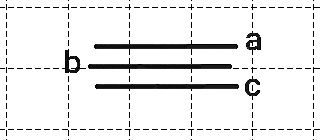
\includegraphics[width=3.9cm]{./img/b0epgTransparenciaGrade2} & &
    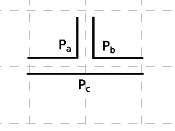
\includegraphics[width=3.5cm]{./img/b1EpgTransparenteGrade2}
    \\
    \footnotesize
    (a) The  graph $C_3$. && \footnotesize(b) $B_0$-EPG representation of $C_3$ (edge-clique).&& \footnotesize(c) $B_1$-EPG representation of $C_3$ (claw-clique).\\
  \end{tabular}

 \caption{The  graph $ C_3 $  and  representations without bends and with 1 bend.} \label{fig:trianguloepgRepresentacao}
\end{figure}


The \emph{bend number} of a graph $G$ is the smallest $k$ for which $G$ is a $B_k$-EPG graph. Analogously, the bend number of a class of graphs is the smallest $k$ for which all graphs in the class have a $B_k$-EPG representation. Interval graphs have bend number $0$, trees have bend number $1$, see~\cite{golumbic2009}, and outerplanar graphs have bend number $2$, see~\cite{daniel2014b}. The bend number for the class of planar graphs is still open, but according to \cite{daniel2014b}, it is either $3$ or $4$.

The class of EPG graphs has been studied in several papers, such as \cite{alcon2016, Asinowski2009, cohen2014, golumbic2009, heldt2014,  martin2017,golumbic2019edge}, among others. The investigations regarding EPG graphs frequently approach characterizations concerning the number of bends of the graph representations. Regarding the complexity of recognizing $B_k$-EPG graphs, only the complexity of recognizing a few of these sub-classes of EPG graphs have been determined: $B_0$-EPG graphs can be recognized in polynomial time, since it corresponds to the class of interval graphs, see ~\cite{booth1976}; in contrast, recognizing $B_1$-EPG and $B_2$-EPG graphs are NP-complete problems, see~\cite{heldt2014} and \cite{martin2017}, respectively. 
Also, note that the paths in a $B_1$-EPG representation have one of the following shapes: $\llcorner$, $\lrcorner$, $\ulcorner$ and $\urcorner$. \cite{cameron2016edge} showed that for each $S\subset \{\llcorner, \lrcorner, \ulcorner, \urcorner\}$, it is NP-complete to determine if a given graph $G$ has a $B_1$-EPG representation using only paths with shape in $S$.

A  collection $C$ of sets satisfies the Helly property when every sub-collection of $C$ that is pairwise intersecting has at least one common element. 
The study of the Helly property is useful in diverse areas of science. We can enumerate applications in semantics, code theory, computational biology, database, image processing, graph theory, optimization, and linear programming, see \cite{dourado2009}.

The Helly property can also be applied to the $B_k$-EPG representation problem, where each path is considered a set of edges. A graph $G$ has a  Helly-$B_k$-EPG representation if there is a $B_k$-EPG representation of $G$ where each path has at most $k$ bends, and this representation satisfies the Helly property. Figure~\ref{fig:envelopeRepresentacoes}(a) presents two $B_1$-EPG representations of a graph with five vertices.  Figure~\ref{fig:envelopeRepresentacoes}(b)   illustrates 3 pairwise intersecting paths ($P_{v_1}, P_{v_2}, P_{v_5}$), containing a common edge, so it is a Helly-$B_1$-EPG representation. In Figure~\ref{fig:envelopeRepresentacoes}(c), although the three paths are pairwise intersecting, there is no common edge in all three paths, and therefore they do not satisfy the Helly property.

The Helly property related to EPG representations of graphs has been studied in~\cite{golumbic2009} and~\cite{golumbic2013}. 

Let $\cal {F}$ be a family of subsets of some universal set $U$, and $h\geq 2$ be an integer.  Say that $\cal{F}$ is $h$-{\it intersecting} when every group of $h$ sets of $\cal {F}$ intersect. The {\it core} of $\cal {F}$, denoted by $core(\cal F)$, is the intersection of all sets of $\cal {F}$. The family $\cal{F}$ is $h$-{\it Helly} when every $h$-intersecting subfamily $\cal{F'}$ of $\cal{F}$ satisfies $core(\cal{F'}) \neq \emptyset$, see e.g. \cite{D76}. On the other hand, if for every subfamily $\cal{F'}$ of $\cal{F}$, there are $h$ subsets whose core equals the core of  $\cal {F'}$, then $\cal {F}$ is said to be {\it strong} $h$-{\it Helly}.
Note that the Helly property that we will consider in this paper is precisely the property of being 2-Helly. 

The  {\it Helly number} of the family $\cal{F}$ is the least integer $h$, such that $\cal{F}$ is $h$-Helly. Similarly, the {\it strong Helly number} of $\cal{F}$ is the least $h$, for which  $\cal{F}$ is strong $h$-Helly. It also follows that the strong Helly number of $\cal{F}$ is at least equal to its Helly number. In~\cite{golumbic2009} and~\cite{golumbic2013}, they have determined the strong Helly number of $B_1$-EPG graphs. 


\begin{figure}[h]
  \centering
  \begin{tabular}{ p{3.2cm} p{4.5cm} p{4.5cm} }
    \centering 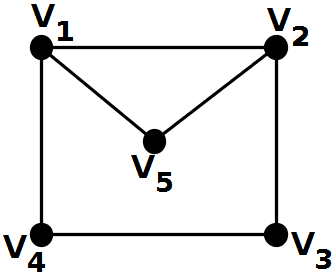
\includegraphics[width=3cm]{./img/envelope} & 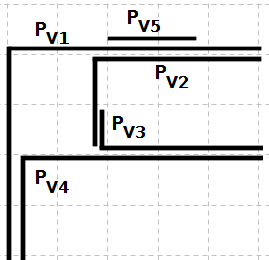
\includegraphics[width=4cm]{./img/envelopeHellyGradeTransparente} & 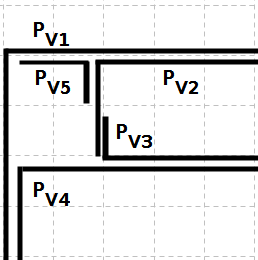
\includegraphics[width=4cm]{./img/envelopeNaoHellyGrade}
    \\
    \footnotesize \centering (a) A  graph with 5 vertices. & \footnotesize(b) A $B_1$-EPG representation that satisfies the Helly property. & \footnotesize (c) A $B_1$-EPG representation that does  not satisfy the Helly property.  \\

  \end{tabular}
\caption{A  graph with 5 vertices in (a) and some single bend representations: Helly in (b) and not Helly in (c).} \label{fig:envelopeRepresentacoes}
\end{figure}

%%%%%%%%%%%%%%%%%%%%%%%%%%%%%%%%%%%%%%%%%%%%%%%%%%%%%%%%%%%%%


Next, we describe some terminology and notation.

The term \emph{grid} is used to denote the Euclidean space of integer orthogonal coordinates. Each pair of integer coordinates corresponds to a \emph{point} (or vertex) of the grid. The \emph{size} of a grid is its number of points. The term \emph{edge of the grid} will be used to denote a pair of vertices that are at a distance one in the grid. Two edges $e_1$ and $e_2$ are \emph{consecutive edges} when they share exactly one point of the grid.
 A (simple) path in the grid is as a sequence of distinct edges $e_1, e_2, \leq, e_m$,  where consecutive edges are adjacent, i.e., contain a common vertex, whereas non-consecutive edges are not adjacent.  In this context, two paths only intersect if they have at least a common edge. The first and last edges of a path are called \emph{extremity edges}.
  
The \emph{direction of an edge} is vertical when the first coordinates of its vertices are equal, and is horizontal when the second coordinates are equal. A \emph {bend} in a path is a pair of consecutive edges $ e_1, e_2 $ of that path, such that the directions of $ e_1$ and $ e_2$ are different. When two edges $ e_1$ and $e_2 $ form a bend, they are called \emph { bend edges}. A \emph {segment} is a set of consecutive edges with no bends. %is a path with no bends.
Two paths are said to be \emph{edge-intersecting}, or simply  \emph{intersecting} if they share at least one edge. Throughout the paper, any time we say that two paths intersect, we mean that they edge-intersect. If every path in a representation of a graph $G$ has at most $k$ bends, we say that this graph $G$ has a \emph{$B_k$-EPG} representation. When $k = 1$ we say that this is a \emph{single bend} representation.

\medskip

In this chapter, we study the Helly-$B_k$-EPG graphs. First, we show that every graph admits an EPG representation that is Helly, and present a characterization of Helly-$B_1$-EPG representations. Besides, we relate Helly-$B_1$-EPG graphs with L-shaped graphs, a natural family of subclasses of $B_1$-EPG. Finally, we prove that recognizing Helly-$B_k$-EPG graphs is in NP, for every fixed $k$. Besides, we show that recognizing Helly-$B_1$-EPG graphs is NP-complete, and it remains NP-complete even when restricted to 2-apex and 3-degenerate graphs.

The rest of the chapter is organized as follows. In Section~\ref{sec:prelim}, we present some preliminary results, we show that every graph is a Helly-EPG graph, present a characterization of Helly-$B_1$-EPG representations, and relate Helly-$B_1$ EPG with L-shaped graphs. In Section~\ref{sec:NPpert}, we discuss the NP-membership of {\sc Helly-$B_k$ EPG Recognition}. In Section~\ref{sec:sectionDispositivoClausula}, we present the NP-completeness of recognizing Helly-$B_1$-EPG graphs. Finally, in the last section the reader can find the complete paper accepted to  journal Discrete Mathematics \& Theoretical Computer Science (DMTCS) that contains the set of proofs that have been omitted from the text.


\section{Preliminaries} \label{sec:prelim}

Before leaving for more laborious results to obtain, let us first notice a simple result. We can observe that when we do not restrict the number of bends of each path, we can show that any graph can be represented as an EPG graph.

This study starts with the following lemma.

\begin{lemma}[\citet{golumbic2009}] \label{lem:todoGrafoEpg}
 Every graph is an EPG graph.
 \end{lemma}
 
 Moreover, the same applies to EPG-Helly graphs. 
 
In an equivalent way, it is also possible to show that every graph has an EPG representation that satisfies the Helly property. An algorithm that performs this construction is presented in the Lemma~\ref{lem:todoGrafoEpgHelly}.

 \begin{lemma}\label{lem:todoGrafoEpgHelly}
 Every graph is a Helly-EPG graph.
 \end{lemma}

\begin{proof}
Let $G$ be a graph with $n$ vertices $v_1, v_2, \dots, v_n$ and $\mu$ maximal cliques $C_1, C_2, \dots , C_{\mu }$. We construct a Helly-EPG representation of $G$ using a $\mu +1\times \mu +1$ grid $Q$. 
%The rows and columns correspond to each maximal cliques and are numbered $1, 2, \dots , \mu$. 
Each maximal clique $C_i$ of $G$ is mapped to an edge of $Q$ as follow: 
\begin{itemize}
    \item if $i$ is even then the maximal clique $C_i$ is mapped to the edge in column $i$ between rows $i$ and $i+1$;
    \item if $i$ is odd then the maximal clique $C_i$ is mapped to the edge in row $i$ between columns $i$ and $i+1$.
\end{itemize}

The following describes a descendant-stair-shaped construction for the paths.
  
Let $v_l \in V(G)$ and $C_i$ be the first maximal clique containing $v_l$ according to the increasing order of their indices. If $i$ is even (resp. odd) the path $P_l$ starts in column $i$ (resp. in row $i$), in the point $(i,i)$. Then $P_l$ extends to at least the point $(i+1, i)$ (resp. $(i, i+1)$) proceeding to the until the row (resp. column) corresponding to next maximal clique of the sequence containing $v_l$, we say $C_{j}$.
At this point, we bend $P_l$, which goes to the point $(j,j)$ and repeat the process previously described. 
%
Figure~\ref{fig:gradeDemonstracao} shows the Helly-EPG representation of the octahedral graph $O_3$, according to the construction previously described.

By construction, each path travels only rows and columns corresponding with maximal cliques containing its respective vertex. And, every path crosses the edges of the grid to which your maximal cliques were mapped. Thus, the previously described construction results in an EPG representation of $G$, which is Helly since every set ${\mathcal P}$ of paths representing a maximal clique has at least one edge in its core.
\end{proof}
 
 \begin{figure}[htb]	
\center%6.3
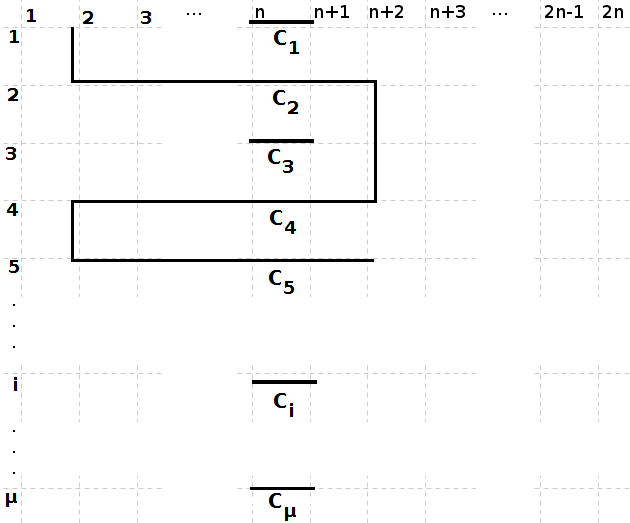
\includegraphics[width=8cm]{./img/grade3.png}
%clausulaGadgetGFCompletaSBPO
\caption{Representação do caminho $P_2$ correspondendo ao vértice $v_2$ contido nas cliques maximais $C_2, C_4$ e $C_5$}
\label{fig:gradeDemonstracao}
\end{figure}


 The provided construction in Lemma~\ref{lem:todoGrafoEpgHelly} can be modified to represent an monotonic row-ascendant EPG representation how in~\cite{golumbic2009} and~\cite{golumbic2013}. To do this, it is enough to change the orientation of the y-axis such that it grows from bottom to up.

%   The Helly property related to EPG representations of graphs has been studied in~\citet{golumbic2009,golumbic2013}.

\begin{definition}
The \emph{Helly-bend number} of a graph $G$, denoted by $b_H(G)$, is the smallest $k$ for which $G$ is a Helly-$B_k$-EPG graph. Also, the bend number of a graph class ${\mathcal C}$ is the smallest $k$ for which all graphs in ${\mathcal C}$ have a $B_k$-EPG representation.
\end{definition}
 
\begin{corollary}\label{cor:maxCliques}
For every graph $G$ containing $\mu$ maximal cliques, it holds that $b_H(G)\leq \mu -1$. 
\end{corollary}


The proof of Corollary~\ref{cor:maxCliques}  is immediate by the Lemma~\ref{lem:todoGrafoEpgHelly}.

Next, we examine the $B_1$-EPG representations of a few graphs that we employ in our constructions.

\medskip

Given an EPG representation of a graph $G$, for any grid edge $e$, the set of paths containing $e$ is a clique in $G$; such a clique is called an edge-clique. A claw in a grid consists of three grid edges meeting at a grid point. The set of paths that contain two of the three edges of a claw is a clique; such a clique is called a claw-clique, see~\cite{golumbic2009}. Fig.~\ref{fig:trianguloepgRepresentacao} illustrates an edge-clique and a claw-clique.

\begin{lemma}[\citet{golumbic2009}]\label{edge-claw-clique} 
Consider a $B_1$-EPG representation of a graph $G$. Every clique in $G$ corresponds to either an edge-clique or a claw-clique.
\end{lemma}

Next, we present a characterization of Helly-$B_1$-EPG representations.

\begin{lemma}\label{caracterization}
A $B_1$-EPG representation of a graph $G$ is Helly if and only if each clique of $G$ is represented by an edge-clique, i.e., it does not contain any claw-clique.
\end{lemma}

The Lemma~\ref{caracterization} is useful to prove that we can check if a given $B_1$-EPG representation is Helly. Just check each clique. 

Now, we consider EPG representations of $C_4$.

\begin{definition} \label{defi:tortasFrame}
Let $ Q $ be a grid and let $ (a_1, b),$ $(a_2, b),$ $(a_3, b),$ $(a_4, b)$ be a 4-star as depicted in Figure~\ref{fig:piesInGrid2}(a). Let $ \mathcal{P} = \{P_1, \dots , P_4\}$ be a collection of distinct paths each containing exactly two edges of the $4$-star.
\begin{itemize}
\item A \emph{true pie} is a representation where each $P_i$ of $ \mathcal{P} $ forms a bend in $b$.

\item A \emph {false pie} is a representation where two of the paths $P_i$ do not contain bends, while the remaining two do not share an edge. 
\end{itemize}
\end{definition}

Fig.~\ref{fig:piesInGrid2} illustrates true pie and false pie representations of a $C_4$.

\begin{figure}[htb]
  \centering
%segundo bloco de figuras
  \begin{tabular}{c c c c c }
    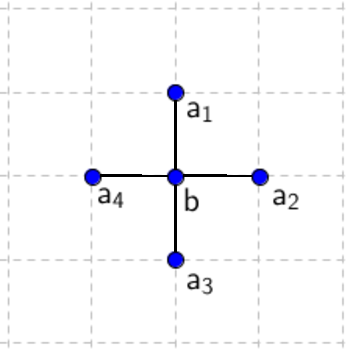
\includegraphics[width=3.5cm]{./img/disposicaoTortaGrid3}    
    & &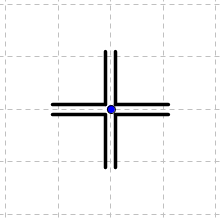
\includegraphics[width=3.5cm]{./img/truePieGrid} 
    & &
 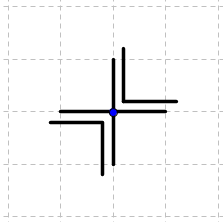
\includegraphics[width=3.5cm]{./img/falsePieGrid} \\%[\abovecaptionskip]
    {\footnotesize (a) 4-star in grid.}  & &  {\footnotesize (b) True pie.} & & {\footnotesize (c) False pie.} %\label{fig:frame}
  \end{tabular}
  \caption{$B_{1}$-EPG representation of the induced cycle of size 4 as pies with emphasis in center $b$.}\label{fig:piesInGrid2}
\end{figure} 


\begin{definition} \label{defi:tortasFrame2}
 Consider a rectangle of any size with 4 corners at points $ (x_1, y_1);$ $(x_2, y_1);$ $(x_2, y_2);$ $(x_1, y_2) $, positioned as in  Fig.~\ref{fig:frameInGrid}(a). 
 \begin{itemize}
 \item A \emph{frame} is a representation containing 4 paths $\mathcal{P} =  \{ P_1, \dots, P_4\} $, each having a bend in a different corner of a rectangle, and such that the  sub-paths $ P_1 \cap P_2, P_1 \cap P_3, P_2 \cap P_4, P_3 \cap P_4 $ share at least one edge. While $P_1 \cap P_4 $ and $ P_2 \cap P_3$ are empty sets.
 
 \item A square-frame is a frame where $P_1$, $P_2$, $P_3$ and $P_4$ have respectively point of bend $ (x_1, y_1),$ $(x_2, y_1),$ $(x_1, y_2)$ and $(x_2, y_2)$, and are of the shape $\llcorner$, $\lrcorner$, $\ulcorner$ and $\urcorner$.  (see Fig.\ref{fig:frameInGrid})
 \end{itemize}
\end{definition}

Fig.~\ref{fig:frameInGrid} illustrates some frame representations of a $C_4$.





\begin{figure}[htb]
  \centering
  \begin{tabular}{c c c c c }
    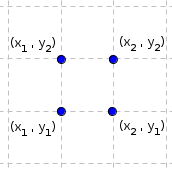
\includegraphics[width=3.5cm]{./img/dispositionFrameInGrid}    
    & &
   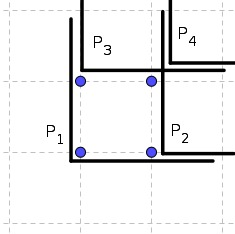
\includegraphics[width=3.5cm]{./img/frame2} 
     & &
   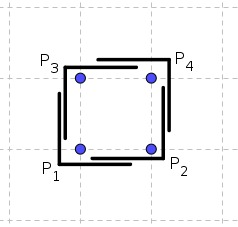
\includegraphics[width=3.5cm]{./img/square2} \\%[\abovecaptionskip]
   {\footnotesize (a) Coordinates of bends of a frame}  
   & & {\footnotesize (b) An example of a frame} 
   & & {\footnotesize (c) A square-frame} %\label{fig:frame}
  \end{tabular}
  \caption{$B_{1}$-EPG representation of the induced cycle of size 4 as frame}\label{fig:frameInGrid}
\end{figure} 


\begin{lemma}[\citet{golumbic2009}]\label{lem:representacaoC4}
Every  $C_4$ that is an induced subgraph of a graph $ G $ corresponds, in any representation, to a true pie, a false pie, or a frame.
\end{lemma}

The following is a claim of~\cite{heldt2014} which a reasoning can be found in~\cite{Asinowski2009}.

\begin{lemma}[\citet{daniel2014b} and \citet{Asinowski2009}]\label{fact:k24facts}
In every single bend representation of a $K_{2,4}$, the path representing each vertex of the largest part has its bend in a false pie.
\end{lemma} %fac

By creating four $K_{2,4}$ and identifying a vertex of the largest part of each one to a distinct vertex of a $C_4$, we construct the graph called bat graph (see Fig~\ref{fig:grafoQ}). Regarding to such a graph, the following holds.

\begin{figure}[htb]
  \centering
  \begin{tabular}{c c c c c }
    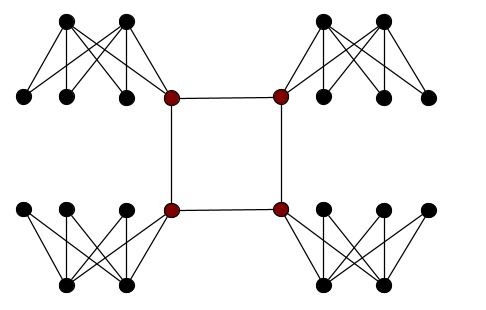
\includegraphics[width=5.5cm]{./img/Qexemplo}    
    & &
   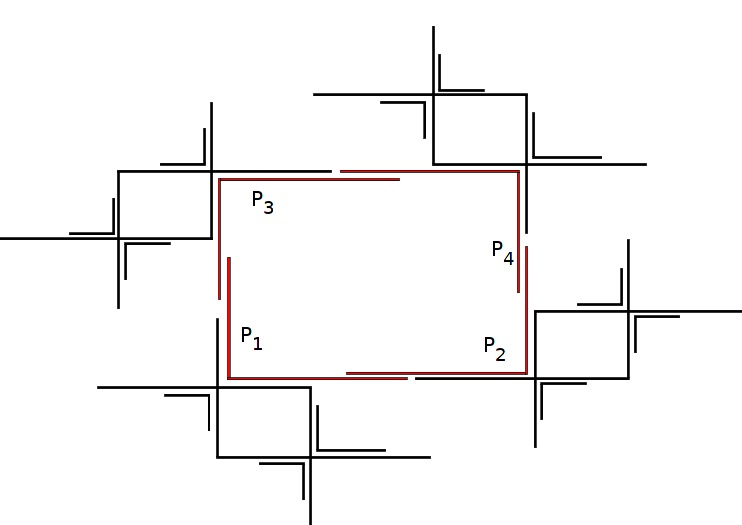
\includegraphics[width=8cm]{./img/representationQ}
  \end{tabular}
  \caption{A bat graph $G$ and a Helly-$B_1$-EPG representation of $G$.}\label{fig:grafoQ}
\end{figure} 

\begin{corollary}\label{batgraph}
In every single bend representation of the bat graph, $G$ presented in Fig.~\ref{fig:grafoQ}, the $C_4$ that is a transversal of all $K_{2,4}$ is represented by a square-frame.
\end{corollary}


\begin{figure}[htb]
  \centering
  \begin{tabular}{c c c c c }
   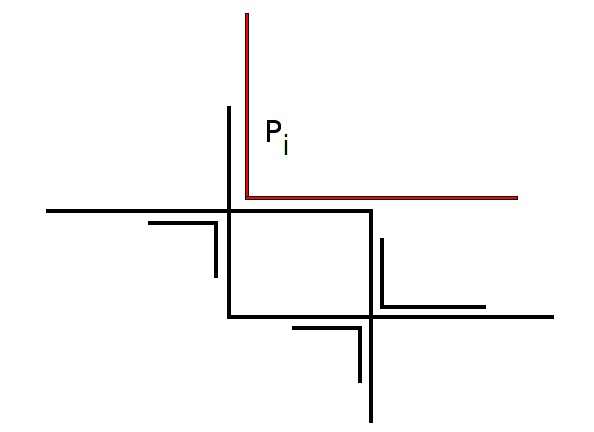
\includegraphics[width=5cm]{./img/representationQ2}
  \end{tabular}
  \caption{Helly-$B_1$-EPG representation of a $K_{2,4}$.}\label{fig:grafoQ2}
\end{figure} 

Figure~\ref{fig:grafoQ2} is an $B_1$-EPG representation for a $K_{2,4}$ graph. We know that any representation of a $K_{2,4}$ has the same shape for vertices in largest set, i.e. bending in a false pie. This fact is fundamental for the construction of a $B_1$-EPG representation of the bat graph, see Figure~\ref{batgraph}. When  we positioned a path $P_i$ corresponding to a vertex of the largest part of $K_{2,4}$ in construction of the bat graph, then we can state that the bend edge of each path $P_i$ does not be used by any non-member of this $K_{2,4}$. Thus each $P_i$ has to intersect another members of this $C_4$ by an extremity edge. Thus, we conclude that each path representing a vertex of the $C_4$ (transversal to all $K_{2,4}$) has its bend in a false pie and this $C_4$ is represented by a square-frame.

\begin{definition}
A $B_k$-EPG representation is \emph{minimal} 
when its set of edges does not properly contain another $B_k$-EPG representation. 
\end{definition}

The \textit{octahedral} graph is the graph containing 6 vertices and 12 edges, depicted  in Figure~\ref{fig:octaedro}(a). Next, we consider representations of the octahedral graph.
 

The next lemma follows directly from the discussion presented in~\cite{heldt2014}.

\begin{lemma}\label{lem:octaedronaohelly}
Every minimal $B_1$-EPG representation of the octahedral graph $O_3$ has the same shape.
\end{lemma}

 
\begin{figure}[h]
  \centering
  
%segundo bloco de figuras
  \begin{tabular}{@{}c@{} p{1.5cm} @{}c@{} }
   \centering 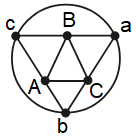
\includegraphics[width=2.5cm]{./img/octaedro.png} & &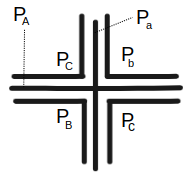
\includegraphics[width=4cm]{./img/representacaoOctaedro.png}  \\[\abovecaptionskip]
    \footnotesize \centering (a) O grafo octaedro $O_3$   & &  \footnotesize(b) Representação $B_1$-EPG do grafo $O_3$
  \end{tabular}

 \caption{O grafo octaedro $O_3$ e sua representação $B_1$-EPG}\label{fig:octaedro}
\end{figure}

The true pie presented in Figure~\ref{fig:octaedro}(b) is composite by paths corresponding to the vertex set $\{b, B, c, C\}$ of the Figure~\ref{fig:octaedro}(a). But in another $B_1$-EPG representation other paths corresponding to a different set of vertices could form the true pie, in any case, yet the shape is maintained. 



\section{Subclasses of $B_1$-EPG graphs}


By Lemma~\ref{lem:octaedronaohelly}, every minimal $B_1$-EPG representation of the octahedral graph $O_3$ has the same shape, as depicted in Fig.~\ref{fig:octaedro}(b). 
Since in any representation of the graph $O_3$ there is always a triple of paths that do not satisfy the Helly property, paths $P_{a}, P_{b} $ and $P_{c}$ in the case of Fig.~\ref{fig:octaedro}(b), it holds that $O_3 \notin$ Helly-$B_1$ EPG, which implies that the class of Helly-$B_1$-EPG graphs is a proper subclass of $B_1$-EPG.

It is easy to see that any $B_0$-EPG representation is Helly. Thus, $B_0$-EPG and Helly-$B_0$-EPG graphs coincide.  Hence, Helly-$B_0$ EPG can be recognized in polynomial time, see \cite{booth1976}.

In a $B_1$-EPG representation of a graph, the paths can be of the following four shapes: $\llcorner$, $\lrcorner$, $\ulcorner$ and $\urcorner$. \citet{cameron2016edge} studied $B_1$-EPG graphs whose paths on the grid belong to a proper subset of the four shapes. If $S$ is a subset of $\{\llcorner, \lrcorner, \ulcorner, \urcorner\}$, then $[S]$ denotes the class of graphs that can be represented by paths whose shapes belong to $S$, where zero-bend paths are considered to be degenerate $\llcorner$'s. They consider the natural subclasses of $B_1$-EPG: $[\llcorner], [\llcorner, \ulcorner], [\llcorner, \urcorner]$ and $[\llcorner, \ulcorner, \urcorner]$, all other subsets are isomorphic
to these up to 90 degree rotation. \cite{cameron2016edge}  showed that recognizing each of these classes is NP-complete.

The following shows how these classes relate to the class of Helly-$B_1$-EPG graphs.
%%%%%%%%%%%%%%

%\begin{figure}[htb]	
\center%6.3
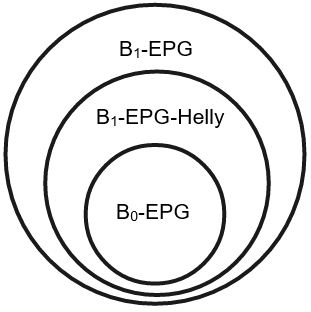
\includegraphics[width=3.5cm]{./img/diagramaClassesEPG.png}
\caption{Diagrama hierárquico de algumas classes  EPG}
\label{fig:diagramaEPG}
\end{figure}
\begin{figure}[H]	
\center%6.3
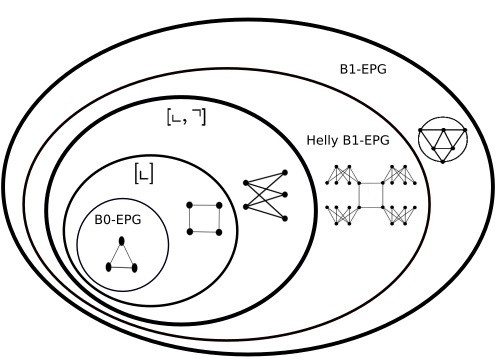
\includegraphics[width=8.5cm]{./img/classes} %2
\caption{Hierarchical diagram of some EPG classes.}
\label{fig:diagramaEPG}
\end{figure}

\begin{theorem}\label{theo:HellyLShaped}
$[\llcorner]\subsetneq [\llcorner, \urcorner]\subsetneq$~Helly-$B_1$ EPG, and Helly-$B_1$ EPG is incomparable with $[\llcorner, \ulcorner]$ and $[\llcorner, \ulcorner, \urcorner]$.
\end{theorem}

The demonstration of Theorem~\ref{theo:HellyLShaped} use statements of \cite{cameron2016edge} about $L$-shaped paths, it also use the bat graph representation (see Fig.~\ref{fig:grafoQ}) and Corollary~\ref{batgraph} and results known to Helly graphs. 

Figure~\ref{fig:diagramaEPG} depicts example of graphs of the classes $B_0$-EPG, $[\llcorner]$, $[\llcorner, \urcorner]$, Helly-$B_1$ EPG, and $B_1$-EPG that distinguish these classes.

It is known that recognizing $[\llcorner]$, $[\llcorner, \urcorner]$, and $B_1$-EPG are NP-complete while recognizing $B_0$-EPG and EPG graphs can be done in polynomial time (c.f.~\cite{booth1976}, \cite{heldt2014}, and \cite{cameron2016edge}).

Although the classes $ B_1$-EPG and Helly-$B_1$ EPG are distinct, the same is not true for the classes $B_0$-EPG and Helly-$B_0 $ EPG, because any $B_0$-EPG representation is Helly.  The $B_0$-EPG class corresponds exactly to class of interval graphs, see~\citet{booth1976}. Throughout the text we will show that each class of Helly-$B_k$ EPG is contained in the corresponding non-Helly class for all $ k \geq 1$, i.e. Helly-$B_k$ EPG $ \subsetneq$ $B_k$-EPG.

In following sections we show that it is NP-complete to recognize Helly-$B_1$-EPG graphs.


\section{Membership in $\mathcal{NP}$} \label{sec:NPpert}

%In this paper we are interested in characterizing the complexity of the $B_1$-EPG-Helly recognition problem, whose formal definition is presented next:
In this section, we will show that the (Helly-)$B_k$-EPG graph recognition problem belongs to $\mathcal{NP}$, when $k$ is polynomial in size with respect to $ |V(G)|$. The problem can be formally described as follows.

% \begin{table}[h!]
% \centering
% %\caption{My caption}
% %\label{my-label}
% \begin{tabular}{ll}
% \hline \hline
% \multicolumn{2}{c}{\sc Reconhecimento $B_k$-EPG-Helly}                         \\ \hline \hline 
% \emph{Entrada}: & Um grafo $G$, e um inteiro $k$.\\
%  & \\
% \emph{Objetivo}: & \begin{tabular}[c]{@{}p{12.5cm}}
% Determinar se existe um conjunto de caminhos $\mathcal{P} = \{P_1, P_2, \ldots, P_n\}$, com até $k$-dobras,  em uma grade  $ Q $ 
% tal que: \\
% \ \ $\bullet$ $v_i, v_j\in V(G)$ são adjacentes se e somente se  $P_i,P_j$ compartilham uma aresta em $Q$; \\
% \ \ $\bullet$ $\mathcal{P}$ satisfaz à propriedade Helly.
% \end{tabular} \\ \hline
% \end{tabular}
% \end{table}



\begin{table}[h!]
\centering
%\caption{My caption}
%\label{my-label}
\begin{tabular}{ll}
\hline \hline
\multicolumn{2}{c}{\sc Helly-$B_k$ EPG Recognition}                         \\ \hline \hline 
\emph{Input}: & A graph $G$ and an integer $k \leq |V(G)|^c$, for some fixed $c$.\\
~ & ~ \\
\emph{Goal:}  & \begin{tabular}[c]{@{}p{9.5cm}}
Determine if there is a set of $k$-bend paths \\ $\mathcal{P} = \{P_1, P_2, \ldots, P_n\} $ in a grid $ Q $ 
such that:\\ 
$\bullet$ \ \ \ $u,v\in V(G)$ are adjacent in $G$ if only if $P_u,P_v$\\ \hspace{0.6cm} share an edge in $Q$; and\\
$\bullet$ \ \ \ $\mathcal{P}$ satisfies the Helly property.
\end{tabular} \\ \hline
\end{tabular}
\end{table}


A (positive) certificate for the {\sc Helly-$B_k$ EPG recognition} consists of a grid $Q$, a set $\mathcal{P}$ of $k$-bend paths on $Q$, which is in one-to-one correspondence with the vertex set $V(G)$ of $G$, such that, for each pair of distinct paths $P_i, P_j\in \mathcal{P}, P_i\cap P_j \neq \emptyset $ if and only if the corresponding vertices are adjacent in $G$. Furthermore, $\mathcal{P}$ satisfies the Helly property.


The following are key concepts that make it easier to control the size of an EPG representation. A \emph{relevant edge} of a path in a $B_k$-EPG representation is either an extremity edge or a bend edge of the path. Note that each path with at most $k$ bends can have up to $2(k + 1)$ relevant edges, and any $B_k$-EPG representation contains at most $2|\mathcal{P}|(k + 1)$ distinct relevant edges. 


To show that there is a non-deterministic polynomial-time algorithm for {\sc Helly-$B_k$ EPG recognition}, it is enough to consider as certificate a  $B_k$-EPG representation $R$ containing a collection $\mathcal{P}$ of paths, $|\mathcal{P}| = |V(G)|$, such that  each path $P_i \in \mathcal{P}$ is given by its set of relevant edges along with the relevant edges, that intersects $P_i$, of each path $P_j$ intersecting $P_i$, where $P_j \in \mathcal{P}$.  The relevant edges for each path are given in the order that they appear in the path, to make straightforward checking that the edges correspond to a unique path with at most $k$ bends.  This representation is also handy for checking that the paths form an intersection model for $G$.

To verify in polynomial time that the input is a positive certificate for the problem, we must assert the following:

\begin{enumerate}%[label=(\roman*)]
\item[(i)] The sequence of relevant edges of a path $P_i\in \mathcal{P}$ determines $P_i$ in polynomial time; \label{it:bullet1}

\item[(ii)] Two paths $P_i, P_j \in \mathcal{P}$ intersect if and only if they intersect in some relevant edge; \label{it:bullet2}

\item[(iii)] The set $\mathcal{P}$ of relevant edges satisfies the Helly property.  \label{it:bullet3}
\end{enumerate}


%The following lemma shows condition~\ref{it:bullet1} holds.

The following lemma states that condition~(i) holds. 



\begin{lemma}\label{lem:verify1}
Each path $P_i$ can be uniquely determined in polynomial time by the sequence of its relevant edges.
\end{lemma}
\begin{proof}
%It is easy to verify that~\ref{it:bullet1} is true, 
Consider the sequence of relevant edges of some path $P_i\in \mathcal{P}$. Start from an extremity edge of $P_i$. Let $t$ be the row (column) containing the last considered relevant edge. The next relevant edge $e'$ in the sequence, must be also contained in row (column) $t$. If $e'$ is an extremity edge, the process is finished, and the path has been determined. It contains all edges between the considered relevant edges in the sequence. Otherwise, if $e'$ is a bend edge, the next relevant edge is the second bend edge $e''$ of this same bend, which is contained in some column (row) $t'$. The process continues until the second extremity edge of $P_i$ is located. 

With the above procedure, we can determine in $\mathcal{O}(k\cdot |V(G)|)$ time, whether path $P_i$ contains any given edge of the grid $Q$. Therefore, the sequence of relevant edges of $P_i$ uniquely determines $P_i$.
 \end{proof}

Next, we assert property~(ii).

\begin{lemma}\label{lem:relevantEdges}
Let $\mathcal{P}$ be the set of paths in a $B_k$-EPG representation of $G$, and let $P_1, P_2\in \mathcal{P}$. Then $P_1$, $P_2$ are intersecting paths if and only if their intersection contains at least one relevant edge.
\end{lemma}

\begin{proof}
 %If $P_1, P_2$ contain a common relevant edge there is nothing to prove. Otherwise,
Assume that $P_1, P_2$ are intersecting, and we show they contain a common relevant edge. Without loss of generality, suppose $P_1, P_2$ intersect at row \textit{i} of the grid, in the  $B_k$-EPG representation $R$. The following are the possible cases that may occur:

\begin{itemize}
\item \textbf{Case 1:} Neither $P_1$ nor $P_2$ contain bends in row \textit{i}. 

Then $P_1$ and $ P_2$  are entirely contained in row \textit{i}. Since they intersect, either $P_1, P_2$  overlap, or one of the paths contains the other. In any of these situations, they intersect in a common extremity edge, which is a relevant edge.

\item \textbf{Case 2:} $P_1$ does not contain bends in \textit{i}, but $ P_2$ does.

If some bend edge of $P_2$ also belongs to $P_1$, then $P_1, P_2$  intersect in  a relevant edge. Otherwise, since $P_1, P_2$  intersect, the only possibility is that the intersection contains an extremity edge of $P_1$ or $ P_2$. Hence the paths intersect in a relevant edge.  

\item \textbf{Case 3:} Both $P_1$,  $P_2$ contain bends in \textit{i}

Again, if the intersection occurs in some bend edge of $P_1$  or $P_2$, the lemma follows. Otherwise, the same situation as above must occur: $P_1, P_2$  must intersect in an extremity edge.
 
\end{itemize}
In any of the cases, $P_1$ and $P_2$ intersect in some relevant edge.
 \end{proof}
 
 
The two previous lemmas let us check that a certificate is an actual $B_k$-EPG representation of a given graph $G$.  The next lemma says we can also verify in polynomial time that the representation encoded in the certificate is a Helly representation. Fortunately, we do not need to check every subset of intersecting paths of the representation to make sure they have a common intersection. 

% \begin{enumerate}[label=\roman*]
% \setcounter{enumi}{2}
% \item The set $\mathcal{P}$ of relevant edges satisfies the Helly property. The following lemma shows the above condition.
% \end{enumerate}

\begin{lemma}\label{lem:verify3}
%Let $\mathcal{P}$ be the set of relevant edges of a $B_k$-EPG representation $R$ of a graph $G$. We can verify that $R$ is Helly representation in polynomial time.
Let $\mathcal{P}$ be a collection of paths encoded as a sequence of relevant edges that constitute a  $B_k$-EPG representation of a graph $G$. We can verify in polynomial time if $\mathcal{P}$ has the Helly property.
\end{lemma}
%\setcounter{proof}{2}

\begin{proof}
%Let $\mathcal{T}$ be the set of relevant edges of $R$. We consider each triple $T_i$ of edges of $\mathcal{T}$. Let $\mathcal{P}_i$ be the set of paths of $R$ containing at least two the relevant edges of $T_i$. By Gilmore's Theorem~\cite{bergeDuchet1975} the paths of $\mathcal{P}_i$  contain a common edge if only if  $R$ is a Helly representation.  By Lemma~\ref{lem:relevantEdges} they contain a common relevant edge. Since there is a polynomial number of relevant edges, we can identify such a common edge, in polynomial time, and confirm that $R$ is in fact Helly. Since the number of triples is also polynomial, the lemma follows.
Let $T$ be the set of relevant edges of $\mathcal{P}$. Consider each triple $T_i$ of edges of $T$ . Let $P_i$ be the set of paths of $\mathcal{P}$ containing at least two of the edges in the triple  $T_i$. By Gilmore's Theorem, see \cite{bergeDuchet1975}, $\mathcal{P}$ has the Helly property if an only if the subset of paths $P_i$  corresponding to each triple  $T_i$  has a non-empty intersection.  By Lemma~\ref{lem:relevantEdges}, it suffices to examine the intersections on relevant edges. Therefore a polynomial algorithm for checking if $\mathcal{P}$ has the Helly property could examine each of the subsets $P_i$, and for each relevant edge $e$ of a path in $P_i$, to compute the number of paths in $P_i$ that contain $e$. Then  $\mathcal{P}$ has the Helly property if and only if for every  $P_i$,  there exists some relevant edge that is present in all paths in $P_i$,  yielding a non-empty intersection.
 \end{proof}

\begin{corollary}\label{cor:comumAtodos}
Let ${\mathcal P'}$ be a set a pairwise intersecting paths in a Helly-$B_k$-EPG representation of a graph $G$. Then the intersection of all paths of  ${\mathcal P'}$ contains at least one relevant edge.
\end{corollary}

Note that the property described in Corollary~\ref{cor:comumAtodos} is a consequence of Gilmore's Theorem, see~\cite{bergeDuchet1975}, and it applies only to representations that satisfy Helly's property.

From Corollary~\ref{cor:comumAtodos}, the following theorem concerning the Helly-bend number of a graph holds.

\begin{theorem}\label{teo:lowerboundCliques}
For every graph $G$ containing $n$ vertices and $\mu$ maximal cliques, it holds that $$\frac{\mu}{2n}-1\leq b_H(G)\leq \mu -1.$$ 
\end{theorem}
\begin{proof}
The upper bound follows from Corollary~\ref{cor:maxCliques}.
For the lower bound first notice that each path with at most $k$ bends can have up to $2(k + 1)$ relevant edges, and any $B_k$-EPG representation with a set of paths $\mathcal{P}$ contains at most $2|\mathcal{P}|(k + 1)$ distinct relevant edges. Now, let $G$ be a graph with $n$ vertices, $\mu$ maximal cliques, and $b_H(G)=k$. From Corollary~\ref{cor:comumAtodos}, it follows that in a Helly-$B_k$-EPG representation of $G$ every maximal clique of $G$ contains at least one relevant edge. By maximality, two distinct maximal cliques cannot share the same edge-clique. Thus, in a Helly-$B_k$-EPG representation of $G$ every maximal clique of $G$ contains at least one distinct relevant edge, which implies that $\mu\leq 2n(k+1)$, so $\frac{\mu}{2n}-1\leq b_H(G)$.
\end{proof}


\begin{lemma}\label{lem:gridPolinomial}
Let $G$ be a (Helly-)$B_k$-EPG graph. Then $G$ admits a (Helly-)$B_k$-EPG representation on a grid of size at most $4n(k+1) \times 4n(k+1)$.
\end{lemma}
\begin{proof}
Let $R$ be a $B_k$-EPG representation of a graph $G$ on a grid $Q$ with the smallest possible size.
Let $\mathcal{P}$ be the set of paths of $R$. Note that $|\mathcal{P}|=n$.
A counting argument shows that there are at most $2|\mathcal{P}|(k+1)$ relevant edges in $R$. 
 If $Q$ has a pair of consecutive columns $c_i,c_{i+1}$ neither of which contains relevant edges of $R$, and such that there is no relevant edge crossing from $c_i$ to $c_{i+1}$, then we can contract each edge crossing from $c_i$ to $c_{i+1}$ into single vertices so as to obtain a new  $B_k$-EPG representation of $G$ on a smaller grid, which is a contradiction. An analogous argument can be applied to pairs of consecutive rows of the grid.
 Therefore the grid $Q$ is such that each pair of consecutive columns and consecutive rows of $Q$  has at least one relevant edge of $R$ or contains a relevant edge crossing it.  
  Since $Q$ is the smallest possible grid for representing $G$, then the first row and the first column of $Q$ must contain at least one point belonging to some relevant edge of $R$. 
Thus, if $G$ is $B_k$-EPG then it admits a $B_k$-EPG representation on a grid of size at most $4|\mathcal{P}|(k+1) \times 4|\mathcal{P}|(k+1)$.
Besides, by Corollary~\ref{cor:comumAtodos}, it holds that the contraction operation previously described preserves the Helly property, if any. Hence, letting $R$ be a Helly-$B_k$-EPG representation of a graph $G$ on a grid $Q$ with the smallest possible size it holds that $Q$ has size at most $4|\mathcal{P}|(k+1) \times 4|\mathcal{P}|(k+1)$.\end{proof}

Given a graph $G$ with $n$ vertices and an EPG representation $R$, it is easy to check in polynomial time with respect to $n +|R|$ whether $R$ is a $B_k$-EPG representation of $G$. By Lemma~\ref{lem:gridPolinomial}, if $G$ is a $B_k$-EPG graph then there is a positive certificate (an EPG representation) $R$ of polynomial size  with respect to $k+n$ to the question ``$G\in B_k$-EPG?''. Therefore, Corollary~\ref{BkNP} holds.

\begin{corollary}\label{BkNP}
Given a graph $G$ and an integer $k\geq 0$, the problem of determining whether $G$ is a $B_k$-EPG graph is in NP, whenever $k$ is bounded by a polynomial function of $|V(G)|$.
\end{corollary}

At this point, we are ready to demonstrate the NP-membership of {\sc Helly-$B_k$ EPG recognition}.

\medskip

\begin{theorem}\label{teo:nppertinencia}
{\sc Helly-$B_k$ EPG recognition} is in NP.
\end{theorem}
\begin{proof}
By Lemma~\ref{lem:gridPolinomial} and the fact that $k$ is bounded by a polynomial function of $|V(G)|$, it follows that the collection $\mathcal{P}$ can be encoded through its relevant edges with $n^{\mathcal{O}(1)}$ bits.

Finally, by Lemmas~\ref{lem:verify1}, \ref{lem:relevantEdges} and \ref{lem:verify3}, it follows that one can verify in polynomial-time in the size of $G$ whether $\mathcal{P}$ is a family of paths encoded as a sequence of relevant edges that constitute a Helly-$B_k$-EPG representation of a graph $G$.
\end{proof}

\section{$NP$-Hardness}\label{sec:sectionDispositivoClausula}

Now we will prove that  {\sc Helly-$B_1$ EPG recognition} is NP-complete. For this proof, we follow the basic strategy described in the prior hardness proof of~\cite{heldt2014}. We set up a reduction from {\sc Positive (1 in 3)-3SAT} defined  as follows:

\begin{table}[h!]
\centering
%\caption{My caption}
%\label{my-label}
\begin{tabular}{ll}
\hline \hline
\multicolumn{2}{c}{\sc Positive (1 in 3)-3SAT}                                \\ \hline \hline 
\emph{Entrada}: & \begin{tabular}[c]{@{}p{12.5cm}@{}} Um conjunto $X$ de variáveis positivas; uma coleção $\mathcal{C}=\{C_1,C_2,\ldots,C_m\}$ de cláusulas sobre  $X$ tal que para cada $C_i\in \mathcal{C}$, $|C_i|= 3$.
\end{tabular} \\
 &  \\
\emph{Objetivo}:  & \begin{tabular}[c]{@{}l@{}} %@{}l@{}
Determinar se existe uma atribuição de valores para as variáveis em $ X $\\ de modo que toda cláusula em  $\mathcal{C}$ tem exatamente um literal verdadeiro.
\end{tabular} \\ \hline
\end{tabular}
\end{table}

{\sc Positive (1 in 3)-3SAT } is a well-known NP-complete problem (see \cite{johnson1979}, problem [L04], page 259). Also, it remains NP-complete when the incidence graph of the input CNF (Conjunctive Normal Form) formula is planar, see~\cite{mulzer2008minimum}.

Given a formula $F$ that is an instance of {\sc Positive (1 in 3)-3SAT} we will present a polynomial-time construction of a graph $ G_F$ such that $ G_F \in$ Helly-$B_1$ EPG if and only if $ F $ is satisfiable. This graph will contain an induced subgraph $ G_{C_i}$ with 12 vertices (called \emph {clause gadget}) for every clause $C_i \in \mathcal{C}$, and an induced subgraph (\emph {variable gadget}) for each variable $ x_j$, containing a special vertex  $ v_j$, plus a \emph{base gadget}  with 55 additional vertices.

 
We will use a graph $H$ isomorphic to the graph presented in Figure~\ref{fig:gadgetBase}, as a gadget to perform the proof. For each clause $C_i$ of $F$ of the target problem, we will have a \emph{clause gadget} isomorphic to $H$, denoted by $G_{c_i}$.

\begin{figure}[htb]	
\center%6.3
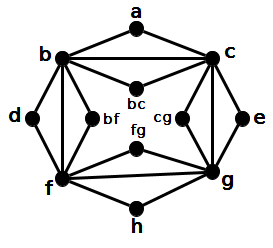
\includegraphics[width=5cm]{./img/gadgetBase.png}
\caption{The partial gadget graph $H$.}
\label{fig:gadgetBase}
\end{figure} 


The reduction of a formula $F$ from  {\sc Positive (1 in 3)-3SAT}  to a particular graph $G_F$ (where $G_F$ has a Helly-$B_1$-EPG representation if only if $F$ is satisfiable) is given below.

\begin{definition}\label{sec:reducao}
Let $F$ be a CNF-formula with variable set $\mathcal{X}$ and clause set $\mathcal{C}$ with no negative literals, in which every clause has exactly three literals. The graph $G_F$ is constructed as follows:

\begin{enumerate}
\item For each clause $C_i \in \mathcal{C}$ create a  \textit{clause gadget} $G_{C_i}$, isomorphic to  graph $H$;

\item For each variable $x_{j}\in \mathcal{X}$ create a \emph{variable vertex} $v_{j}$ that is adjacent to the vertex $a$, $e,$ or $h$ of $G_{C_i}$, when $x_{j}$ is the first, second or third variable in $C_i$, respectively;

\item For each variable vertex $v_{j}$, construct a \emph{variable gadget} formed by adding two copies of $H$, $H_1$ and $H_2$, and making $v_j$ adjacent to the vertices of the triangles $(a, b, c)$ in  $H_1$ and $H_2$.

 %where $v_{j}$ is  adjacent to all vertices of the triangle (a,b,c);%; (c,e,g); (g,f,h); or (b,d,f)) of each $H_1$ and $H_2$; 

%\item The  subgraph induced by \emph{variable vertex}  $v_{j}$, and also $V(H_1)$ and $V(H_2)$ will be called \emph{variable gadget}; 

\item Create a vertex $V$, that will be used as a vertical reference of the construction, and add an edge from $V$ to each vertex $d$ of a clause gadget;%$d \in V(G_c)$;

\item Create a bipartite graph $K_{2,4}$ with a particular vertex $T$ in the largest stable set. This vertex is nominated \emph{true vertex}. Vertex $T$ is adjacent to all $v_{j}$ and also to $V$;

\item Create two  graphs isomorphic to $H$, $G_{B1}$ and $G_{B2}$. The vertex $T$ is connected to each vertex of the triangle (a,b,c) in $G_{B1}$ and $G_{B2}$;


\item Create two graphs isomorphic  to $H$, $G_{B3}$ and $G_{B4}$. The vertex $V$ is connected to each vertex of the triangle (a,b,c) in $G_{B3}$ and $G_{B4}$;

\item The  subgraph induced by the set of vertices $\{V(K_{2,4}) \cup  \{T, V\} \cup V(G_{B1}) \cup V(G_{B2}) \cup V(G_{B3}) \cup V(G_{B4})\}$ will be referred to as the  \emph{base gadget}. 
\end{enumerate}
\end{definition}


Figure~\ref{fig:exemploGrafoGF} illustrates how this construction works on a small formula. 


\begin{figure}[htb]	
\center%6.3
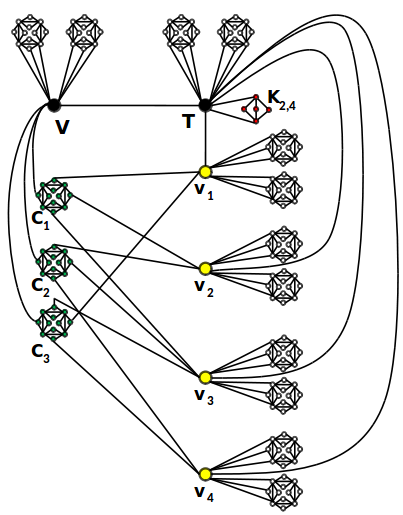
\includegraphics[width=6.5cm]{./img/exemploGrafoGFSBPO4.png}
\caption{O grafo $G_{F}$ correspondendo à fórmula $F=(x_1+ x_2+ x_3) \wedge  (x_2+ x_3+ x_4 )\wedge  (x_3 + x_1 + x_4 )$}
\label{fig:exemploGrafoGF}
\end{figure}

\begin{lemma}\label{lem:ida}
Given a satisfiable instance $F$ of {\sc Positive (1 in 3)-3SAT}, the graph $G_F$ constructed from $F$ according to Definition~\ref{sec:reducao} admits a Helly-$B_1$-EPG representation.
\end{lemma}


Using base, variables and clause gadgets constructed in an appropriate way, it is possible to demonstrate that we can obtain a Helly-$B_1$-EPG representation from the input formula. Figure~\ref{fig:gadgetFormulaCompletaPies} depicts a Helly-$B_1$-EPG representation for the gadget built in Figure~\ref{fig:exemploGrafoGF}. For more proof details see the paper is last section of this chapter.


\begin{figure}[htb]	
\center%6.3
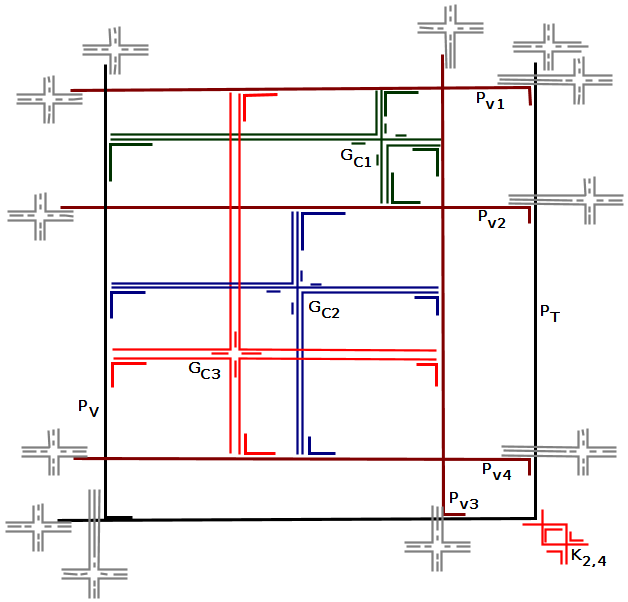
\includegraphics[width=10cm]{./img/formulaFGCompletaPies.png}
%clausulaGadgetGFCompletaSBPO
\caption{Representação de dobra simples de $G_F$}
\label{fig:gadgetFormulaCompletaPies}
\end{figure}

Now, we consider the converse. Let $R$ be a Helly-$B_1$-EPG representation of $G_F$, then we will get the original formula.


\begin{lemma}\label{lem:volta}
If a graph $G_F$, constructed according to Definition~\ref{sec:reducao}, admits a Helly-$B_1$-EPG representation, then the associated CNF-formula $F$ is a yes-instance of {\sc Positive (1 in 3)-3sat}.
\end{lemma}

To obtain the formula $F$ associated with the  representation $R$ of $G_F$, a few steps are necessary: 1 - identify the  clauses gadgets, so you can know how many clauses make up the formula; 2 - identify the variable gadgets, that way you can know which are the variables that make up each clause; 3 - check which variables and clauses gadgets have intersecting paths, so it is possible to identify which variables are in each clause; 4 - check the direction of the intersections among each variable gadget with the base gadget, this makes it possible to identify the value (True/False) of each variable.  This takes us to the next theorem.

\begin{theorem}
{\sc Helly-$B_1$ EPG recognition} is NP-complete.
\end{theorem}
\begin{proof} %\textbf{Proof}.
By Theorem~\ref{teo:nppertinencia}, Lemma~\ref{lem:ida}, Lemma~\ref{lem:volta}.
 \end{proof}



We say that a $k$-apex graph is a graph that can be made planar by the removal of $k$ vertices. A $d$-degenerate graph is a graph in which every subgraph has a vertex of degree at most $d$. Recall that {\sc Positive (1 in 3)-3SAT} remains NP-complete when the incidence graph of the input formula is planar, see~\cite{mulzer2008minimum}. Thus, the following corollary holds.

\begin{corollary}\label{coro:2apexAnd3degenerate}
{\sc Helly-$B_1$ EPG recognition} is NP-complete on $2$-apex and $3$-degenerate graphs.
\end{corollary}

To prove that $G_F$ is 3-degenerate, we apply the $d$-degenerate graphs recognition algorithm. Now, to prove that $G_F$ is $2$-appex when the incidence graph of the input formula is planar, we need to recall that {\sc Positive (1 in 3)-3SAT} remains NP-complete when the incidence graph of $F$ is planar, see~\cite{mulzer2008minimum}. Therefore, is enough to demonstrate that there is a planar arrangement between the intersections of the variable gadgets and clause gadgets, then from that one can construct a graph $G_F$ such that the removal of $V$ and $T$ results into a planar graph. The complete proof is in paper in the last section of this chapter.


\section{Concluding Remarks}

In this chapter, we show that every graph admits a Helly-EPG representation, and $\frac{\mu}{2n}-1\leq b_H(G)\leq \mu -1$. Besides, we relate Helly-$B_1$-EPG graphs with L-shaped graphs, a natural family of subclasses of $B_1$-EPG. Also, we prove that recognizing (Helly-)$B_k$-EPG graphs is in $\mathcal{NP}$, for every fixed $k$. Finally, we show that recognizing Helly-$B_1$-EPG graphs is NP-complete, and it remains NP-complete even when restricted to 2-apex and 3-degenerate graphs.

Now, let $r$ be a positive integer and let $K_{2r}^-$ be the cocktail-party graph, i.e., a complete graph on $2r$ vertices with a perfect matching removed. Since $K_{2r}^-$ has $2^r$ maximal cliques, by Theorem~\ref{teo:lowerboundCliques} follows that $\frac{2^r}{4r}-1\leq b_H(K_{2r}^-)$. This implies that, for each $k$, the graph $K_{2(k+5)}^-$ is not a Helly-$B_k$-EPG graph. Therefore, as \cite{martin2017} showed that every cocktail-party graph is in $B_2$-EPG, we conclude the following.

\begin{lemma}
Helly-$B_k$-EPG $\subsetneq B_k$-EPG for each $k>0$.
\end{lemma}

The previous lemma suggests asking about the complexity of recognizing Helly-$B_k$-EPG graphs for each $k>1$. Also, it seems interesting to present characterizations for Helly-$B_k$-EPG representations similar to Lemma~\ref{caracterization} (especially for $k=2$) as well as considering the $h$-Helly-$B_k$ EPG graphs. Regarding L-shaped graphs, it also seems interesting to analyse the classes Helly-$[\llcorner, \ulcorner]$ and Helly-$[\llcorner, \ulcorner, \urcorner]$ (recall Thereom~\ref{theo:HellyLShaped}).




\section{Article accepted for publication in the journal  Discrete Mathematics \& Theoretical Computer Science (DMTCS)} 
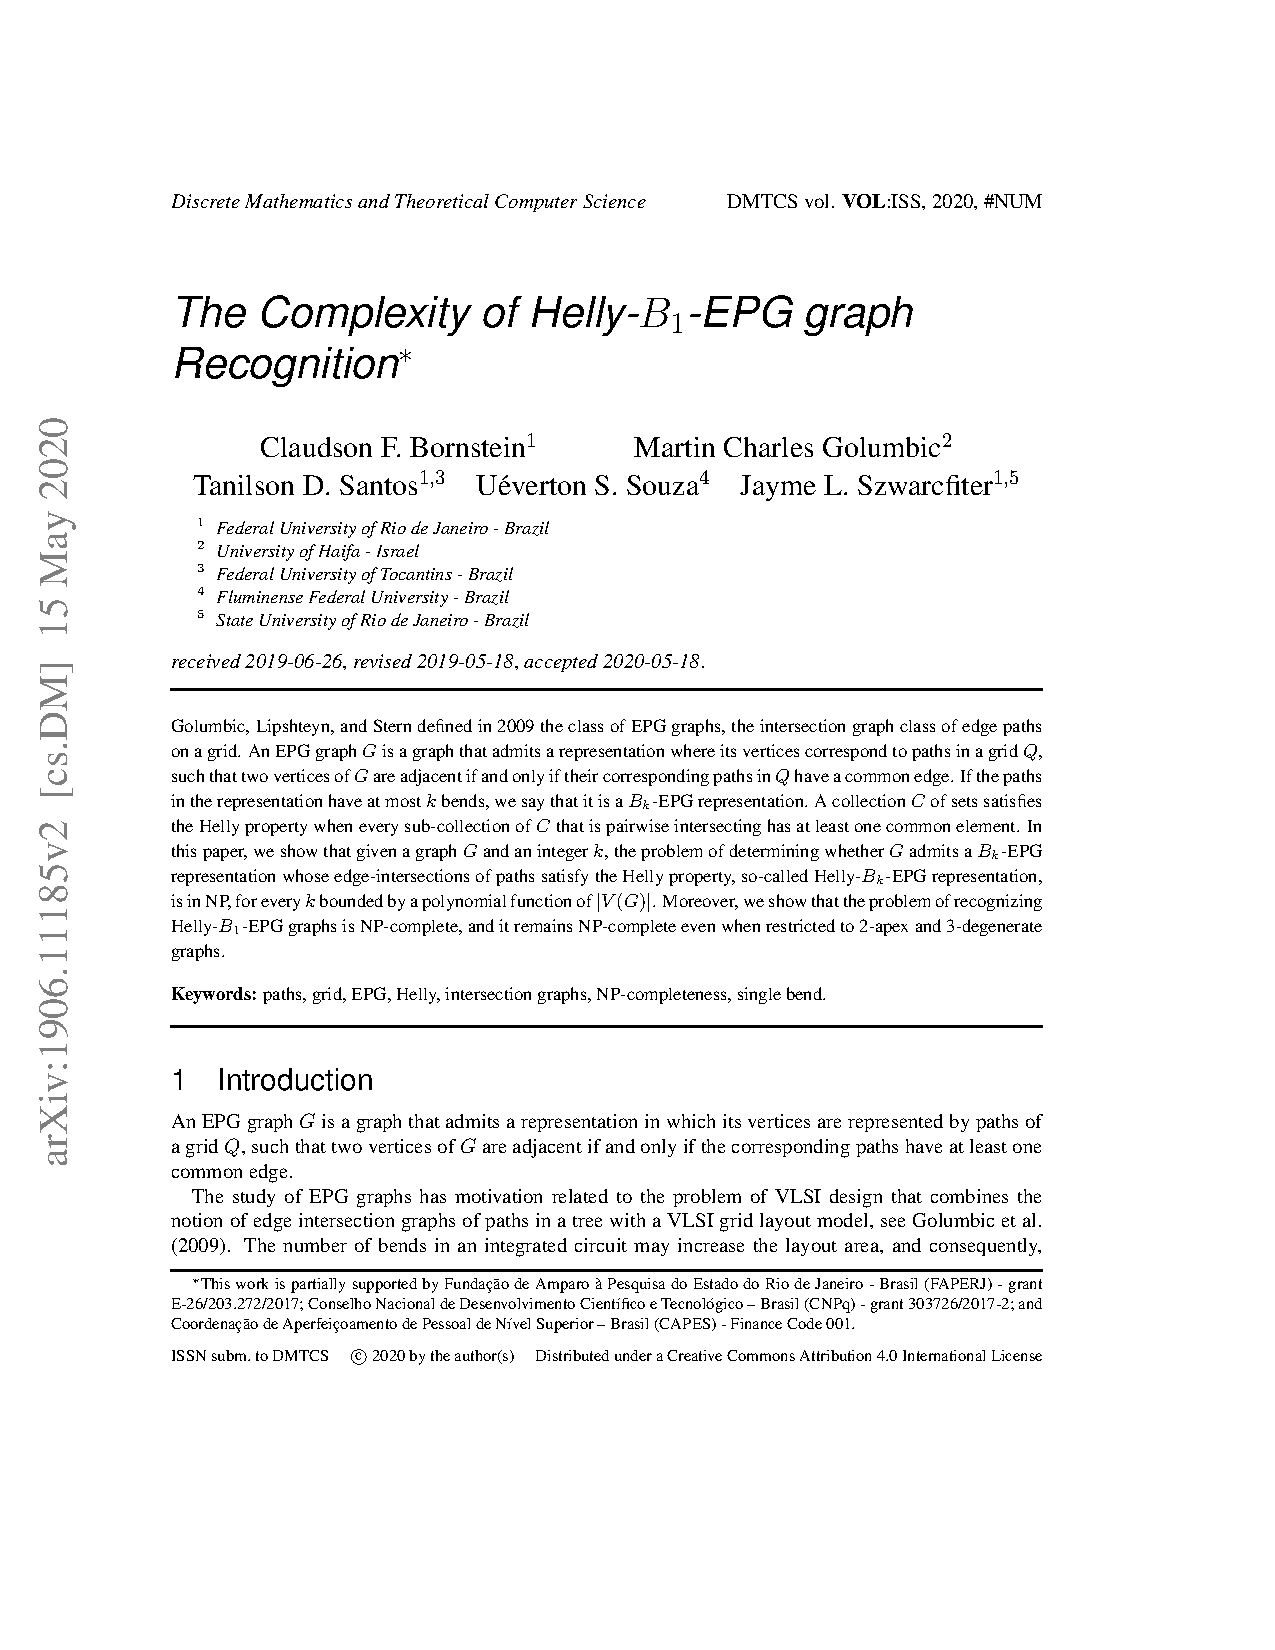
\includepdf[pages=-]{./includes/include-pdf-files/dmtcsTanilson.pdf}
  \chapter{The Helly and Strong Helly numbers for graphs $B_k$-EPG and $B_k$-VPG}
\label{cap:iv}

\begin{flushright}
\begin{minipage}[t][0cm][b]{0.47\textwidth}
\emph{
%A Matemática é o alfabeto com o qual Deus escreveu o Universo.
Falta algo para completar esta demonstração, mas não tenho tempo.}
\end{minipage}

\rule[0cm]{7cm}{0.03cm}%{largura}{espessura}

Évariste Galois
\end{flushright}


EPG graphs were introduced by \citet{golumbic2009} and consist of the intersection graphs of sets of paths on the orthogonal grid, whose intersections are taken considering the edges of the paths. If the intersections of the paths consider the vertices and not the edges, the resulting graph class is called VPG graphs. This last class was introduced in 2011 by \citet{asinowski2011string} e \citet{asinowski2012}.  In this chapter we investigate two parameters in both graph classes, EPG and VPG. The parameters that will be studied are namely the Helly number and the strong Helly number. The parameter strong Helly number  generalizes the parameter Helly number. Thus, by definition the Helly number is a natural lower bound for the strong Helly number in any family of sets studied. In this chapter, we solve the problem of determining both the Helly and strong Helly numbers, for $B_k$-EPG, and $B_k$-VPG graphs, for each value $k$. In last section of this chapter the reader can find a complete version of the paper submitted to  the journal DMGT that contains the set of proofs that have been omitted from the text.






\section{Introduction}

%\footnote{
%$1$ Federal University of Rio de Janeiro, Brazil \\
%$^2$ University of Haifa, Israel \\
%$^3$ Holon Institute of Technology, Israel \\
%$^{1,4}$ Federal University of Tocantins, Brazil \\
%$^5$ Federal Fluminense University, Brazil \\
%$^6$ State University of Rio de Janeiro, Brazil}

%EPG graphs were by \item 
EPG graphs were introduced by Golumbic, Lypshteyn, and Stern (2009) and consist of the intersection graphs of sets of paths on the orthogonal grid, whose intersections are taken considering the edges of the paths. If the intersections of the paths consider the vertices and not the edges, the resulting graph class is called VPG graphs. Such a class was introduced in 2011 \cite{asinowski2011string} and \cite{asinowski2012}.  In the present chapter, we study two graph parameters of both EPG and VPG graphs, namely the Helly number and the strong Helly number.

Let $\cal {F}$ be a family of subsets of some universal set $U$, and $h$ an integer $\geq 1$.  Say that $\cal{F}$ is $h$-{\it intersecting} when every group of $h$ sets of $\cal {F}$ intersect. The {\it core} of $\cal {F}$ is the intersection of all sets of $\cal {F}$, denoted $core(\cal F)$. 

The family $\cal{F}$ is $h$-{\it Helly}  when every $h$-intersecting subfamily $\cal{F'}$ of it satisfies $core(\cal{F'}) \neq \emptyset$, see e.g. \cite{duchet1978propriete}. On the other hand, if for every subfamily $\cal{F'}$ of $\cal{F}$, there are $h$ subsets whose core equals the core of  $\cal {F'}$, then $\cal {F}$ is said to be {\it strong} $h$-{\it Helly}. Clearly, if $\cal {F}$ is $h$-Helly then it is $h'$-Helly, for $h' \geq h$. Similarly, 
 if ${\cal F}$ is strong $h$-Helly then it is strong $h'$-Helly, for $h' \geq h$. 

Finally, the  {\it Helly number} of the family $\cal{F}$ is the least integer $h$, such that $\cal{F}$ is $h$-Helly. Similarly, the {\it strong Helly number} of $\cal{F}$ is the least $h$, for which  $\cal{F}$ is strong $h$-Helly. It also follows that the strong Helly number of $\cal{F}$ is at least equal to its  Helly number.


A {\it class} $\cal {C}$ of families $\cal {F}$  of subsets of some universal set $U$ is a subcollection  of the families  $\cal {F}$ of $U$. Say that $\cal C$ is a {\it hereditary} class when it closed under inclusion. The {\it Helly number} of a class $\cal{C}$ of families $\cal{F}$ of subsets is the largest Helly number among the families $\cal {F}$. Similarly, the {\it strong Helly number} of a class $\cal {C}$ is the largest strong Helly number of the families of $\cal {C}$.

If $\cal F$ is a family of subsets and $\cal C$ a class of families, denote by $H(\cal F)$ and 
$H(\cal C)$,  the Helly numbers of $\cal F$ and $\cal C$, respectively, while  $sH({\cal F})$ and $sH({\cal C})$  represent the strong Helly numbers of $\cal F$ and $\cal C$.


In this chapter, we study families of subsets $\cal{F}$ of edge and vertex paths in a grid. In the context of edge paths, a path consists of a sequence of consecutive edges in the orthogonal grid. We call a collection of such paths an {\it EPG representation}, i.e., a collection of paths that represent a graph via its intersection graph (considering edge intersections). {\it EPG graphs} are the class of graphs that admit an EPG representation.
Similarly, for vertex paths, a path consists of a sequence of consecutive vertices of the orthogonal grid and a collection of
these paths form a {\it VPG representation} and correspond to a {\it VPG graph}. 

Each edge has an associated direction in the grid, which can be either horizontal or vertical. A {\it bend} in a path is a pair of consecutive edges that have different directions. A {\it segment} of a path is a sequence of consecutive edges of the path, with no bends. Say that a path $P_i$ is a $B_k$-{\it path} if it contains at most $k$ bends. Say that $\cal {F}$ is a  $B_k$-paths family, or simply a $B_k$-family,  if each path of $\cal {F}$ is a $B_k$-path. 

 In this chapter, we solve the problem for determining the Helly and strong Helly numbers, for both $B_k$-EPG and $B_k$-VPG graphs, for each value $k$.

For EPG graphs,  the Helly number of  $B_0$-families is well known and is equal to 2, since $B_0$-EPG graphs coincide with interval graphs. It is also simple to conclude that the strong Helly number of $B_0$-EPG graphs are also equal to 2. For $k = 1$,  
we prove that both the Helly number and the strong Helly number of the class of $B_1$-families are equal to 3. For the class of $B_2$-families, we prove that these two parameters are equal to 4. The Helly and strong Helly number for $B_3$-families equal 8, and finally, these parameters are unbounded for $k \geq 4$. 

As for VPG graphs, it is simple to verify that the Helly number of $B_0$-VPG graphs equals 2, and we prove that $B_1$-VPG have Helly number 4, $B_2$-VPG graphs have Helly number 6, $B_3$-VPG has Helly number 12, while the Helly number for $B_4$-VPG graphs is again unbounded. 

Finally, the strong Helly number equals the Helly number of $B_k$-EPG graphs, for each $k$. Similarly, for $B_k$-VPG graphs. 

As for existing results, 
Golumbic, Lipshteyn, and Stern \cite{golumbic2009}  have already shown that the strong Helly number for $B_1$-EPG graphs equal 3, and for $B_1$-VPG graphs is equal to 4. employing a different proof technique. See  \cite{chung201950}, Theorem 11.13, below:
\begin{theorem}\label{thm:chung201950}{\cite{chung201950}}
Let $P$ be a collection of single bend paths on a grid. If every two paths in $P$ share at least one grid-edge, then $P$ has strong Helly number 3. Otherwise, $P$ has strong Helly number 4.
\end{theorem}
No other results concerning the strong Helly number, or no results for the Helly number of $B_k$-EPG graphs seem to have been reported in the literature. As for other classes, Golumbic and Jamison have determined the strong Helly number of the intersection of edge paths of a tree \cite{golumbic1985}. Finally, Asinowski, Cohen, Golumbic, Limouzy, Lipshteyn, and Stern have reported that the strong Helly number of $B_0$-VPG graphs equals two \cite{asinowski2011string}.  

Deciding whether a given hypergraph is $k$-Helly can be done in polynomial time for fixed $k$, employing the characterization by Berge and Duchet \cite{bergeDuchet1975}. For arbitrary $k$, the problem is co-NP-complete \cite{dourado2009}. For the corresponding problems for strong $k$-Helly see \cite{dourado2008strong,dourado2009}.

The chapter is organized as follows. Section~\ref{sec:preliminares4} contains some preliminary propositions and further notation. Section~\ref{sec:Helly-number} describes the results for the Helly number of $B_k$-EPG graphs, while Section~\ref{sec:HellynumberVPG} contains the results of this parameter for $B_k$-VPG graphs. The strong Helly number is considered in Section~\ref{sec:strongHellyNumber}. Following, we present the final remarks in Section~\ref{sec:concludingRemarks} and in the last section appear the paper submitted to the journal Discussiones Mathematicae Graph Theory (DMGT).




\section{Preliminaries}\label{sec:preliminares4}

The following theorem characterizes $h$-Helly families of subsets.


\begin{theorem}\label{thm:BD}(\cite{bergeDuchet1975}):
A family $\cal{F}$  of subsets of the universal set $U$ is $h$-Helly if and only if for every subset $U' \subseteq U$, $|U'|= h+1$, the subfamily $\cal{F'}$ of $\cal{F}$, formed by the subsets containing at least $h$ of the $h+1$ elements of $U'$, has a non-empty core. 
\end{theorem}

The next theorem is central to our results.

\begin{theorem}\label{thm:minimal}
Let ${\cal C}$ be a hereditary class of families ${\cal F}$ of subsets of the universal set $U$, whose Helly number $H({\cal C})$ equals $h$. Then there exists a family ${\cal F'} \in {\cal C}$ with exactly $h$ subsets, satisfying the following condition: 

For each subset $P_i \in \cal {F'}$, there is exactly one distinct element $u_i \in U$, such that \\
$$u_i \not \in P_i,$$ 
but $u_i$ is contained in all  subsets 
$$P_j \in {\cal F'} \setminus P_i.$$
\end{theorem}
 

Proof: 
Let ${\cal C}$ be a class of families ${\cal F}$ of subsets $P$, each subset formed by elements $u \in U$, such that the Helly number $H({\cal C})$ equals $h$. Then each family ${\cal F} \in {\cal C}$ satisfies $H({\cal F}) \leq h$. Consider a family ${\cal F'} \in {\cal C}$  whose Helly number is exactly $h$, and containing exactly $h$ subsets. Such a family must exist since ${\cal C}$ is hereditary. Since $H({\cal F'}) = h$, $\cal F'$ is $h$-intersecting, and therefore $(h-1)$-intersecting. Furthermore, ${\cal F'}$ is not $(h-1)$-Helly. Applying  Theorem \ref{thm:BD}, we conclude that there are $h$ elements $U' = \{u_1, \ldots, u_h\} \subset U$, such that each set of ${\cal F'}$ contains at least $h-1$ elements of $U'$. Since $H({\cal F'}) > h-1$, $core({\cal F'}) = \emptyset$ and therefore there is no common element among the sets of $\cal F'$. In particular, since each set $P_i \in {\cal F'}$ contains at least $h-1$ elements of $U'$, and $core(\cal F') = \emptyset$, we can choose $h$ subsets $P_i$, in which each of them misses a distinct element $u_i \in U'$. Then for each subset $P_i \in \cal F$, there exists some element $u_i \not \in P_i$, but $u_i \in P_j$, for all $P_j \in \cal F'$, $j \neq i$. \qed

Let $\cal{ F'}$ be as in the previous theorem. It is simple to conclude that the removal of any subset from $\cal {F'}$ makes it an $(h-1)$-Helly family. Therefore we  call $\cal {F'}$ a {\it minimal non}-$(h-1)$-{\it Helly family}. Moreover, the element $u_i \not \in P_i$, contained in all subsets $P_j \in {\cal{F'}} \setminus P_i$, except $P_i$, is the {\it $h$-non-representative} of $P_i$.  

We can apply this notion of minimal families of subsets for the $B_k$-EPG and $B_k$-VPG representations. Recall that $B_k$-EPG and $B_k$-VPG graphs are hereditary classes. 

\section{The Helly Number of $B_k$-EPG Graphs}\label{sec:Helly-number}

In this section, we determine the Helly number of the classes of $B_1$-EPG, $B_2$-EPG and $B_3$-EPG graphs, and show that for $B_k$-EPG graphs, $k \geq 4$, the Helly number is unbounded. We prove the following result.

\begin{theorem}\label{thm:Helly-EPG}
The Helly number of $B_k$-EPG graphs satisfy:
\begin{enumerate}[nosep,label=\emph{(\roman*)}]
\item  $H(B_1$-EPG) = 3.
\item $H(B_2$-EPG)  = 4. 
\item $H(B_3$-EPG)  = 8. 
\item $H(B_k$-EPG) is unbounded, for 
$k \geq 4$.
\end{enumerate}

\end{theorem}

The proof consists in determining tight lower and upper bounds, as shown in the next two subsections. 

\subsection{Lower Bounds}

We present lower bounds for the Helly number, as a function of the number $k$ of bends.

\begin{claim}\label{claim:lower-Bk-EPG} 
The following are lower bounds for $B_k$-EPG graphs.
\begin{enumerate}[nosep,label=\emph{(\roman*)}]
\item   $H(B_1$-$EPG) \geq 3$. 
\item $H(B_2$-$EPG) \geq 4$. 
\item $H(B_3$-$EPG) \geq 8$. 
\item $H(B_k$-$EPG )$ is unbounded for $k \geq 4$.
\end{enumerate}
\end{claim}

For each value of $k$, we exhibit a $B_k$-family of edge paths whose Helly number is the corresponding stated value. In other words, if we can present a family of subsets pairwise intersecting  with $|\mathcal{P}|$ paths, where each path has at most $k$ bends, this means that for this given value of $ k $ the Helly number of $B_k$-EPG is at least $ |\mathcal{P}|$. Figures~\ref{fig:lowerBoundBkEPG1}(a), (b), (c) illustrate path families in $B_1$-EPG, $B_2$-EPG and $B_3$-EPG that have exactly $ |\mathcal{P}|$ paths pairwise intersecting. However, the lower bound for the Helly number in these classes are those described in Lemma
~\ref{claim:lower-Bk-EPG}.

\begin{figure}[!h]
\begin{center}
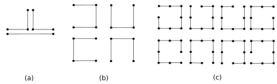
\includegraphics[width=12cm]{./img/b1epgSub.pdf}
\end{center}
\caption{Minimal non-Helly sub-families for the $B_1$, $B_2$ and $B_3$ -families.}
\label{fig:lowerBoundBkEPG1}
\end{figure}

Observe that for $k=4$ we can always to construct families $\cal{F}$ that are $(n-1)$-intersecting, while $core({\cal{F}})=\emptyset$ (see Figure~\ref{fig:lowerBoundB4EPG}). Therefore $H(B_4$-EPG) is unbounded. Clearly the same holds for $k >4$. 

\begin{figure}[!h]
\begin{center}
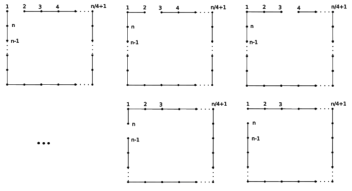
\includegraphics[width=12.5cm]{./img/b4epg.pdf}
\end{center}
\caption{$B_4$-EPG has an unlimited Helly number.}
\label{fig:lowerBoundB4EPG}
\end{figure}

Next, we consider upper bounds for the Helly number $B_k$-EPG graphs.

\subsection{Upper Bounds}\label{subsec-upper}

In order to obtain tight upper bounds for the Helly number, in terms of the number of bends, we introduce below more notation and lemmas.

Say that a set of edges of a grid is {\it co-linear} if all edges of the set belong to the same line of the grid, horizontal or vertical. The set of edges is called {\it parallel} if all its edges lie on parallel lines of the grid, but no two of them are co-linear.  


\begin{lemma}
\label{lemma:3colin}
Let $\cal {F}$ be a minimal non-$(h-1)$-Helly family of paths on a grid containing three co-linear non-representative edges. Then $\cal{F}$ must contain paths with at least four bends.
\end{lemma}



\begin{lemma}
\label{lemma:3par}
Let $\cal{F}$ be a minimal non-$(h-1)$-Helly family of paths on a grid, containing three parallel edges, and having  Helly number $H(\cal{F})$   $\geq 4$. Then $\cal{F}$ must contain paths with at least four bends. 
\end{lemma}


\begin{lemma} \label{lemma:Lwit}
Let $\cal{F}$ be a minimal non-$(h-1)$-Helly family of paths on a grid with  Helly number $H({\cal F}) \geq 4$. If ${\cal F}$ contains three non-representative edges that lie on a common $B_1$-subpath $P_i$, then $\cal {F}$ must have some path with at least three bends. \end{lemma}


The following are tight upper bounds for the Helly numbers of $B_k$-EPG paths, for $k = 1,2,3$.

\begin{claim}\label{claim:upper-B1}
$H(B_1$-$EPG) \leq 3.$
\end{claim}
 
\proof
Assume by contradiction that the Helly number of $B_1$-EPG paths is $h > 3$. In this case, consider a minimal non-$(h-1)$-Helly family of $\cal F$ of $B_1$-EPG paths. Then $\cal F$ contains at least $h$ paths.  
Any path $P_1 \in \cal{F}$ must contain $h-1$ non-representative edges  corresponding to the $h-1$ distinct paths of $\cal F$ other than $P_1$. Since $h-1 \geq 3$, $P_1$ contains at least three distinct non-representative edges $u_2, u_3, u_4 \in P_i$, with $u_3$ lying  between $u_2$ and $u_4$ in the path.   

If $u_2$, $u_3$ and $u_4$ are co-linear then by Lemma~\ref{lemma:3colin} $P_3 \in \cal{F}$ must contain at least four bends. Otherwise, the edges must lie on $P_1$ which has a single bend. Thus, it follows from Lemma~\ref{lemma:Lwit} that $P_3$ has three bends. In any situation, a contradiction arises, implying that $H({\cal F}) \leq 3$.
\qed

\begin{claim}\label{claim:upper-B2}
$H(B_2$-EPG$) \leq 4.$
\end{claim}

\proof
Assume by contradiction that the Helly number of  $B_2$-EPG families of paths is $h > 4$. Consider a minimal non-$(h-1)$-Helly family $\cal F$ of $B_2$-EPG paths. The family  $\cal F$ must contain at least $h \geq 5$ distinct paths, each of them corresponding to a distinct non-representative edge. Choose arbitrarily 5 of these non-representative edges.

By Lemmas ~\ref{lemma:3colin} and ~\ref{lemma:3par} any three of these chosen edges can  neither be co-linear nor parallel. Therefore, at least one of the five chosen non-representative edges must be in a different direction from the majority of the chosen edges. Call the direction of this edge vertical and the direction of the majority of the chosen edges horizontal. Consider a path $P_1$ from the family $\cal F$ that goes through this vertical edge. 
The path $P_1$ contains at least four of the chosen non-representative edges, at least one of which is vertical. Since $P_1$ has at most two bends, then it must have at most three segments. Since we have three segments and four non-representative edges which $P_1$ must contain, by the pigeon hole principle, one of these segments must have two non-representative edges. If this pair of edges are in a horizontal segment of $P_1$, then such pair of edges, along with the vertical edge are in two consecutive path segments, forming a $B_1$-subpath in $\cal F$. Then Lemma~\ref{lemma:Lwit} implies that some path of $\cal F$ must have at least three bends.   Otherwise, the two edges are vertical. But the others must be horizontal, and again we have at least three edges in a pair of consecutive segments forming a subpath in $\cal F$ having one bend. Again,  Lemma ~\ref{lemma:Lwit} implies that some path has at least three bends.
\qed

\begin{claim}\label{claim:upper-B3}
$H(B_3$-EPG$) \leq 8.$
\end{claim}

\proof
Assume by contradiction that the Helly number of  $B_3$-EPG paths is $h > 8$. In this case, consider a minimal non-$(h-1)$-Helly family $\cal F$ of $B_3$-EPG paths. Then $\cal F$ contains at least $h$  distinct non-representative edges,  corresponding to $h$ distinct paths.  By Lemma~\ref{lemma:3par}, since we can have at most three bends in any path, then these $h$  non-representative edges must lie in at most two vertical and two horizontal lines of the grid. Therefore one of these four possible lines must contain at least three distinct non-representative edges. By Lemma~\ref{lemma:3colin},  that would imply the existence of a path with four bends.\qed

This completes the proof of Theorem \ref{thm:Helly-EPG}. 


\section{Helly number of $B_k$-VPG Graphs}\label{sec:HellynumberVPG}

In this section, we determine the Helly number of $B_k$-VPG graphs. We prove the following results.
\begin{theorem}\label{thm:Bk-VPG}
The Helly numbers for $B_k$-VPG graphs satisfy:
\begin{enumerate}
\item $H(B_1$-VPG) = 4.
\item $H(B_2$-VPG) = 6.
\item $H(B_3$-VPG) = 12.
\item $H(B_4$-VPG) is unbounded.
\end{enumerate}
\end{theorem}

Again, we prove the theorem by showing tight lower and upper bounds.

\subsection{Lower Bounds}

%First, we describe lower bounds.
We start by describing some sets of paths that achieve our lower bounds. 
Figure \ref{VPG:lower-B1} shows a set of 4 $B_1$-paths of a graph $G$, in a $2 \times 2$ grid, such that each path covers three vertices of the grid, and avoids exactly one of the vertices. 

\begin{figure}[!h]
    \centering
    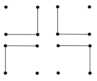
\includegraphics[width=3cm]{./img/lower-bound-B1-VPG.pdf}
    \caption{Lower bound for $B_1$-VPG graphs.}
    \label{VPG:lower-B1}
\end{figure}

Figure \ref{VPG:lower-B2} shows a set of 6 $B_2$-paths of a graph $G$, in a $2 \times 3$ grid, such that each path covers five vertices of the grid, and avoids exactly one. 


\begin{figure}[!h]
    \centering
    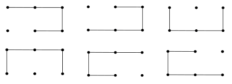
\includegraphics[width=8cm]{./img/lower-bound-B2-VPG.pdf}
    \caption{Lower bound for $B_2$-$VPG$ graphs.}
    \label{VPG:lower-B2}
\end{figure}


Figure \ref{VPG:lower-B3} shows 12 $B_3$-paths of a graph $G$, in a grid, of perimeter 12, such that each path covers 11  vertices of the grid,  avoiding one of them. 

\begin{figure}[!h]
    \centering
    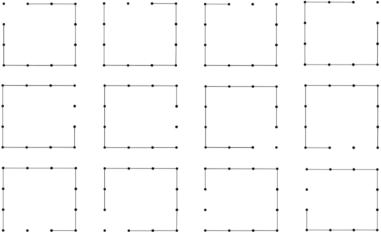
\includegraphics[width=12cm]{./img/lower-bound-B3-VPG.pdf}
    \caption{Lower bound for $B_3$-VPG graphs.}
    \label{VPG:lower-B3}
\end{figure}

Figure \ref{VPG:lower-B4} shows a set of $n$ $B_4$-paths of a $n$-vertex graph $G$, in a grid having perimeter $n$,  such that each path covers $n-1$  vertices of $G$, avoiding one of them. 

\begin{figure}[!h]
    \centering
    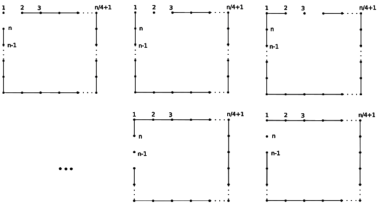
\includegraphics[width=12cm]{./img/lower-bound-B4-VPG.pdf}
    \caption{Lower bound for $B_4$-VPG graphs.}
    \label{VPG:lower-B4}
\end{figure}

Applying Theorem \ref{thm:minimal}, we can then conclude that the number of vertices of each of the above-described graphs is lower bound for the corresponding class. Then, we can claim the following bounds.

\begin{claim}\label{claim:VPG-lower}
The following are lower bounds for the Helly numbers of $B_k$-VPG graphs.
\begin{enumerate}
\item $H(B_1$-VPG) $\geq 4$.
\item $H(B_2$-VPG) $\geq 6$.
\item $H(B_3$-VPG) $\geq 12$.
\item $H(B_4$-VPG) is unbounded.
\end{enumerate}
\end{claim}

\subsection{Upper Bounds}

Next, we provide upper bounds for the Helly number of $B_k$-VPG graphs. The following lemmas are employed.

\begin{lemma}\label{column-sizes}
Let $\cal F$ be a minimal non-$(h-1)$-Helly family of paths, for some $h$, containing $k \in \{3,4,5\}$ distinct co-linear non-representative points of the grid. Then $\cal F$ contains a path having at least $k-1$ bends.
\end{lemma}

% \proof For $k \in \{3,5\}$, the path avoiding the middle point has at least $k-1$ bends, while for $k = 4$, the path avoiding one of the middle points also has this same property.
% \qed

\begin{lemma}\label{column-number}
Let $\cal F$ be a minimal non-$(h-1)$-Helly family of paths, on a grid containing $k < h$ distinct pairwise non-co-linear non-representative points. Then $\cal F$ must contain a path with at least $k-1$ bends.
\end{lemma}   

% \proof Since $k < h$, $\cal F$ must contain a path that visits all such $k$ pairwise non-co-linear points. Such a path requires at least one bend, between two consecutive non-co-linear points. Therefore $\cal F$ contains a path with at least $k-1$ bends. \qed \\

We also employ some additional concepts and notation, below described.

Let $\cal F$ be a minimal non-$(h-1)$-Helly family of $B_{k-1}$-paths on a grid $Q$. By Theorem \ref{thm:minimal},  we can choose $h$ paths $P_i \in {\cal F}$, each of them associated to a distinct non-representative grid point $p_i$, such that $P_i$ avoids $p_i$, but contains all the other $h-1$ distinct non-representative points $p_j \in P_J$, for each   $j \neq i$. Denote by $P_N$, $|P_N|=h$, the subset of grid  points of  $Q$, restricted to the chosen set of distinct  non-representative points $p_i$. By Lemmas \ref{column-sizes} and \ref{column-number}, the grid points of $P_N$ are contained in at most $k$ columns (lines), and each column (line) contains at most $k$ points of $P_N$. Consequently, the cardinalities of the points of $P_N$, contained in the columns (lines) of $Q$,  form a partition of the integer $h$, into at most $k$ parts, such that each part is at most $k$. Call such a partition as a {\it feasible  partition  of $h$, relative to $P_N$}. Therefore, each non-representative point $p_i \in P_N$ contributes with one unit to some part of the partition, which is then referred to,   as the part of the partition {\it corresponding} to $p_i$.    

The following lemma describes sufficient conditions for an integer $h$ to be an upper bound for the Helly number.

\begin{lemma}\label{upper-bound} Let $\cal F$ be a minimal non-$(h-1)$-Helly family of $B_{k-1}$-paths on a grid $Q$, and $P_N$ the set of non-representative points of $Q$. Let $k,h$ be integers, $1 \leq k \leq 3$ and $k < h$. The following conditions imply $H(B_k$-VPG) $\leq h$  
\begin{itemize}
    \item[(i)] there is no feasible partition of $h+1$, relative to $P_N$, or 
    \item[(ii)] for any possible feasible partition, and for any arrangement of the grid points of $P_N$ in $Q$, there is some non-representative point $p_i \in P_N$, such that  no path exists  in $Q$, having at most $k$ bends, containing all points of $P_N$, except $p_i$.    
\end{itemize}
\end{lemma}
{\it Proof}: The proof of (i) follows from Lemmas \ref{column-sizes} and \ref{column-number}, while the proof of (ii) is a consequence of Theorem \ref{thm:minimal}.  \qed \\

The following are upper bounds for the Helly number of $B_k$-VPG graphs, for each $k$, $1 \leq k \leq 3$, obtained  by applying Lemma \ref{upper-bound}.      
 
\begin{claim}\label{claim:upper-B1-VPG}
$H(B_1$-VPG) $\leq  4$.
\end{claim}

% \proof There is no partition of the integer 5, into two parts, in which each part is at most 2. Consequently, the result follows from Lemma \ref{upper-bound} (i). \qed

\begin{claim}\label{claim:upper-B2-VPG}
$H(B_2$-VPG)  $\leq  6$.
\end{claim}

% \proof Assume the contrary. Then $H(B_2$-VPG) $\geq  7$, let $\cal F$ be a minimal non-6-Helly family of $B_2$-paths, and  $P_N$ be the set of non-representative points of $\cal F$ in $Q$. There are two possible partitions of the integer 7, in three parts, each of them of size at most 3, namely $(3,3,1)$ and $(3,2,2)$. In any of these cases,  it is always possible to choose some point  $p_i \in P_N$, belonging to a part of the partition of size 3, such that a path in $\cal F$  which avoids $p_i$ and covers the other six non-representative points, must contain at least three bends.  Then by Lemma \ref{upper-bound}, indeed $H(B_2$-VPG)  $\leq  6$. \qed


\begin{claim}\label{claim:upper-B3-VPG}
$H(B_3$-VPG) $\leq  12$.
\end{claim}

% \proof Assume the contrary, $H(B_3$-VPG) $\geq  12$. Let $\cal F$ be a minimal non-12-Helly family of $B_3$-paths, and  $P_N$ be the set of non-representative points of $\cal F$ in $Q$. There are three possible partitions of the integer 13, into four parts, each of them of size at most 4, namely $(4,4,4,1)$, $(4,4,3,2)$ and $(4,3,3,3)$. In this case, choose $p_i \in P_N$ to be a non-representative point, corresponding to a part of size $4$ of the partition.  The path of ${\cal F}$, which avoids $p_i$, must cover the other 12 non-representative points. These points are located in 4 distinct columns, of cardinalities 4,4,3,1, 4,3,3,2, or 3,3,3,3, considering the three possible partitions, respectively. Such a path must contain at least four bends, a contradiction. Then by Lemma \ref{upper-bound}, $H(B_3$-VPG) $\leq  12$.    \qed  

From the lower and upper bounds described in the previous subsections, we obtain the results for the Helly numbers of $B_k$-VPG graphs, completing the proof of Theorem \ref{thm:Bk-VPG}.

\section{Strong Helly Number} \label{sec:strongHellyNumber}

In this section, we first consider determining the strong Helly number of $B_k$-EPG graphs.

We start by describing a theorem similar to Theorem \ref{thm:minimal}.

\begin{theorem}\label{thm:minimal-strong}

Let ${\cal C}$ be a hereditary class of families $\cal F$ of subsets of the universal set $U$, whose strong Helly number $sH({\cal C})$ equals $h$. Then there exists a family ${\cal F'} \in {\cal C}$ with exactly $h$ subsets satisfying the following condition: 

For each subset $P_i \in \cal {F'}$, there is exactly one distinct element $u_i \in U$, such that \\
$$u_i \not \in P_i,$$ 
but $u_i$ is contained in all  subsets 
$$P_j \in {\cal F'} \setminus P_i.$$
\end{theorem}

Proof: The strong Helly number of ${\cal C}$ is $h$ and not $h - 1$, so that  there must exist some family ${\cal F} \in {\cal C}$ whose strong Helly number is exactly $h$, i.e., $\cal F$  contains $h$ subsets $P_i$ whose intersection equals  core($\cal F'$) but is such that no  $h-1$ of its subsets have the same intersection. In particular, let $\cal F'$ be the family containing exactly the $h$ subsets $P_i$ described above. Such a family must exist, since $\cal C$ is hereditary. Then each $P_i$ does not contain at least one element $u_i$ in the intersection of the remaining $h-1$ subsets $P_j$, $j \ne i$, 
since the intersection of these $h-1$ subsets must not be equal to the core($\cal F'$).  \qed

Again, if we consider the family $\cal F'$ described in the theorem above it is simple to conclude that the removal of any subset from $\cal {F'}$ turns it $(h-1)$-strong Helly.  Then call $\cal {F'}$ a {\it minimal} non-$(h-1)$-strong Helly family. Moreover, the element $u_i \not \in P_i$, contained in all subsets $P_j \in {\cal{F'}} \setminus P_i$, except $P_i$, is the {\it $h$ non-representative} of $P_i$.  

As before, we employ the above minimal families of subsets, applied to paths in a grid.

We prove that the strong Helly number of $B_k$-EPG graphs coincide with the Helly number, for each corresponding value of $k$. Similarly, for $B_k$-VPG graphs. For $k=0$, it is simple to show that if a set of intervals $\cal I$ in a line pairwise intersect, then there exist two intervals of $\cal I$, whose intersection equals the intersection of all intervals of $\cal I$. Consequently, the $k$-strong Helly number of $B_0$-EPG graphs equals 2. 
Similarly, for $B_0$-VPG graphs. 
Recall that the strong Helly number is at least equal to the Helly number of a family so that the lower bounds presented in Claim~\ref{claim:lower-Bk-EPG} also hold for the strong Helly number. The proofs for the strong Helly numbers for $k \geq 1$ are similar to those described in Section \ref{sec:Helly-number}.  



\section{Concluding Remarks}\label{sec:concludingRemarks}
We have determined the Helly number and strong Helly number of $B_k$-EPG graphs and $B_k$-VPG graphs, for $k \geq 0$. 

Table \ref{tab:Helly-Strong-Helly} summarizes the results obtained.
 
\Large 

\begin{table}[htb]
    \centering
    \caption{Helly and Strong Helly Numbers for $B_k$-EPG and $B_k$-VPG Graphs}
    \label{tab:Helly-Strong-Helly}
    \begin{tabular}{c|c|c}
    \cline{1-3} $k$  & $B_k$-EPG & $B_k$-VPG \\
    \cline{1-3} 0 & 2 & 2 \\
    \cline{1-3} 1 & 3 & 4 \\
    \cline{1-3} 2 & 4 & 6 \\
    \cline{1-3} 3 & 8 & 12 \\
    \cline{1-3} $\geq 4$ & unbounded & unbounded \\
    \cline{1-3} 
    \end{tabular}
\end{table}

\normalsize

We leave two questions to be investigated concerning the presented results.

\begin{enumerate}
\item Given a {\it specific}  EPG or VPG graph, the question is to formulate an algorithm to determine its Helly and strong Helly numbers. See \cite{dourado2008improved}, for instance, for such algorithms, applied to general graphs. 

\item The values of the Helly and strong Helly numbers, which were determined in this paper, coincided in all cases. Clearly, in general, this is not the case. We leave as an open question, to find the conditions for such equality to occur. \end{enumerate}


\newpage


\section{Article submitted to journal  Discussiones Mathematicae Graph Theory (DMGT)} 
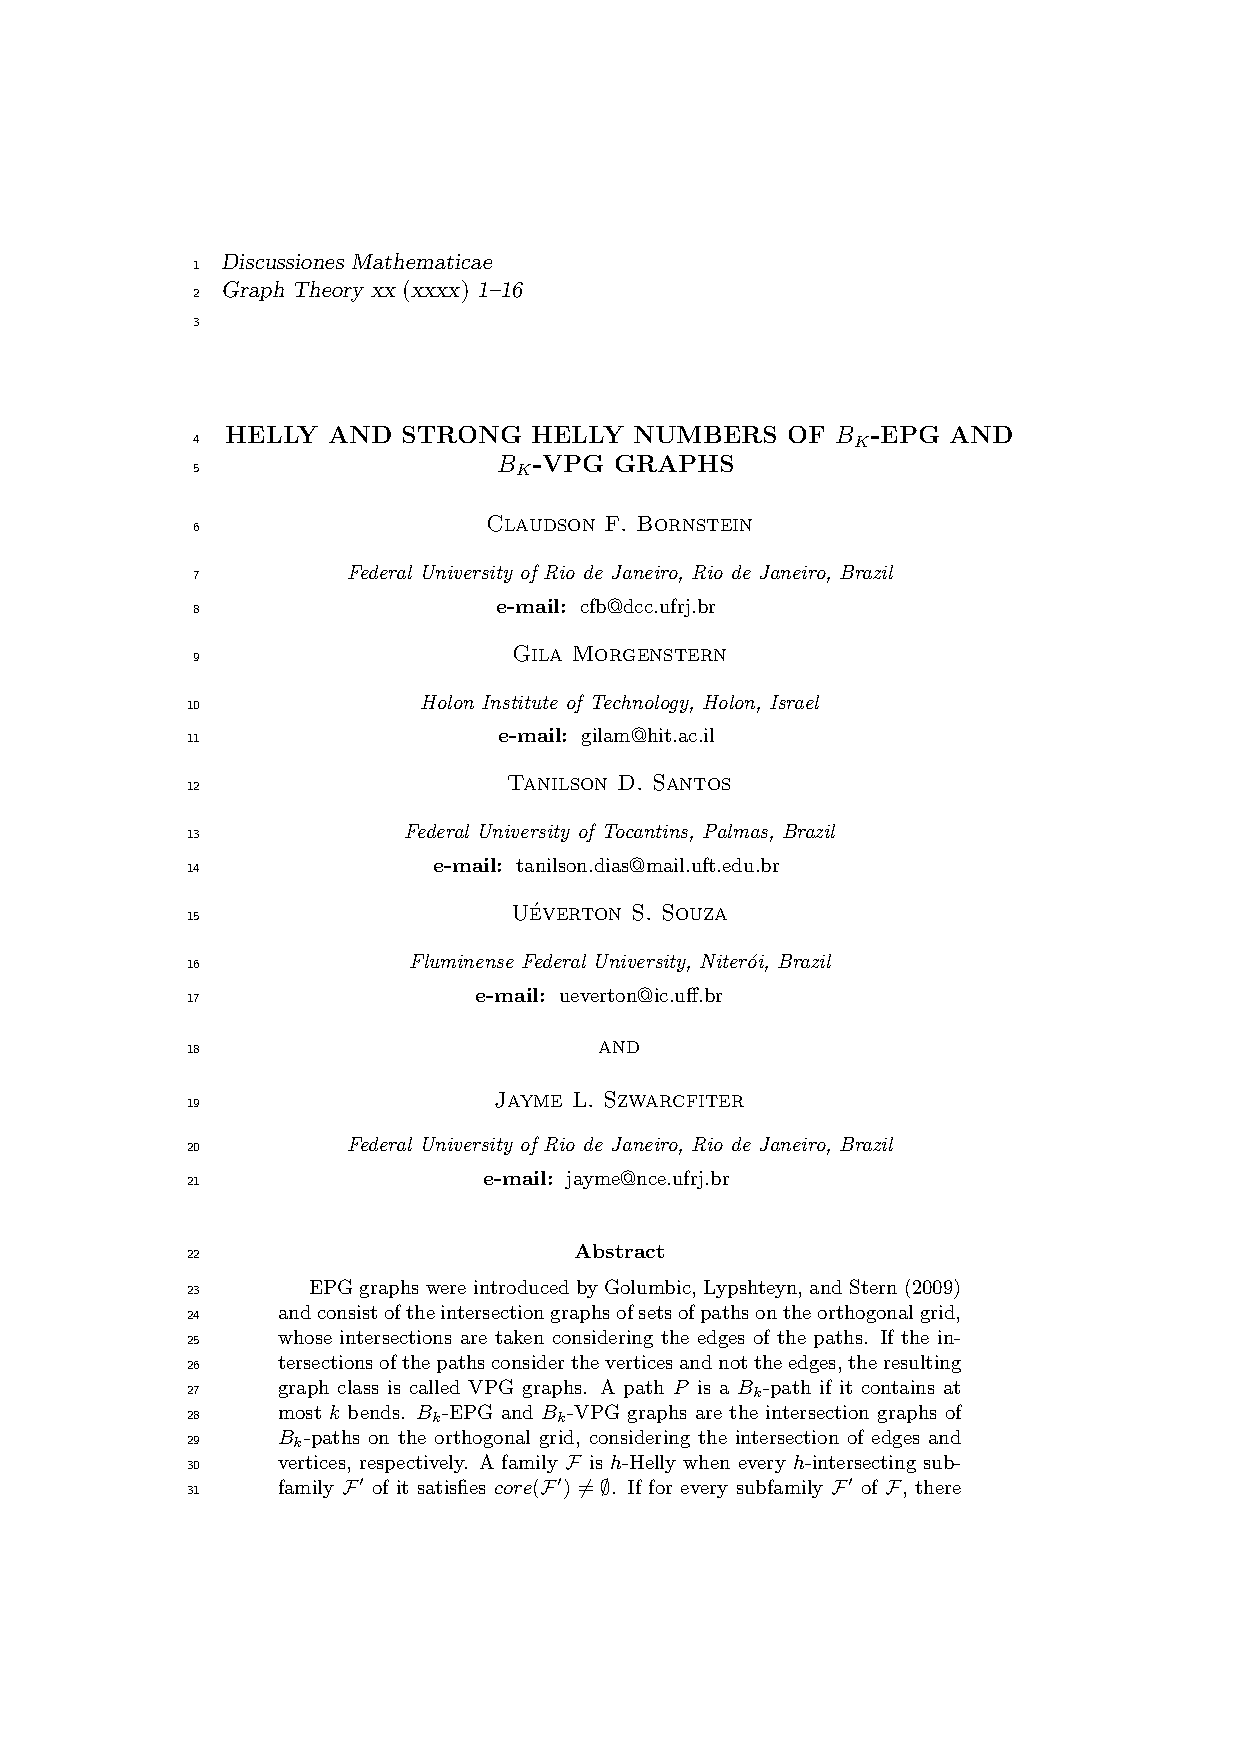
\includepdf[pages=-]{./includes/include-pdf-files/paperDMGT2020.pdf}
  \chapter{Relationship among  $B_1$-EPG, EPT and VPT graph classes}
\label{cap:v}

\begin{flushright}
\begin{minipage}[t][0cm][b]{0.47\textwidth}
\emph{
%A Matemática não mente. Mente quem faz mau uso dela.
What we know is a drop, what we don't know is an ocean.}
\end{minipage}

\rule[0cm]{7cm}{0.03cm}%{largura}{espessura}

%Albert Einstein
Sir Isaac Newton
\end{flushright}

\begin{quotation}
This chapter presents as the main result that every Chordal $B_1$-EPG graph is simultaneously in the VPT and EPT graph classes. In particular, we describe structures that belong to $B_1$-EPG but  do not support a Helly-$B_1$-EPG representation and thus we define some sets of subgraphs that delimit Helly subfamilies. 
 In addition, this chapter also presents features of some non-trivial graph families that are properly contained in Helly-$B_1$ EPG, namely these families are composed of the Bipartite, Blocks, Cactus, and Line of Bipartite  graphs. Finally, at the end of this chapter, the reader can find a section with a complete version of the paper submitted to the journal DMGT that contains the set of proofs that have been omitted from the text.
\end{quotation}


\section{Introduction}

Models based on paths intersection  may consider  intersections by vertices or   intersections by edges.  Cases where the paths are hosted on a tree  appear first in the literature, see for instance \cite{gavril1978recognition, golumbic1985edge, golumbic1985}.  Representations using paths on a grid were considered later, see  \cite{golumbic2009,golumbic2013, golumbic2013intersection}. %More details on each intersection model will be given in the following text.

 Let $P$ be a family of paths on a host tree $T$. Two types of intersection graphs from the pair $<P,T>$ are defined, namely VPT and EPT graphs.
The \textit{edge intersection graph} of $P$, EPT(P), has vertices which correspond to the members of $P$, and two vertices are adjacent in EPT(P) if and only if the corresponding paths in $P$ share at least one edge in T. Similarly, the \textit{vertex intersection graph} of $P$, VPT(P), has vertices which correspond to the members of $P$, and two vertices are adjacent in VPT(P) if and only if the corresponding paths in $P$ share at least one vertex in $T$.
%
VPT and EPT graphs are incomparable families of graphs. However, when the maximum degree of the host tree is restricted to three the family of
VPT graphs coincides with the family of EPT graphs \cite{golumbic1985edge% \cite{alcon2010necessary
}. Also it is known that any Chordal EPT graph is VPT (see~\cite{syslo1985triangulated}). Recall that it was shown that Chordal graphs are the vertex intersection graphs of subtrees of a tree \cite{gavril1974intersection}.


Edge intersection graphs of paths on a grid are called \textit{EPG graphs}. 

In \citeauthor{golumbic2009} \cite{golumbic2009}, the authors proved that every graph is EPG, and started the study of the subclasses
defined bounding the number of times any path used in the representation can to bend.  Graphs admitting a representation
where  paths  have at most $k$ changes of direction  (bends) were called $B_k$-EPG. 
 In particular, when the paths have at most one bend we have the \textit{ $B_1$-EPG graphs} or a \textit{single bend EPG graphs}.

 A pertinent question in the context of path intersection graphs is as follows: given two classes of path intersection graphs,
 the first whose host is a tree and the second whose host is a grid,  is there an intersection or containment relationship among these classes? What do we know about it?

In the present chapter we will explore $B_1$-EPG graphs, in particular diamond-free graphs and Chordal graphs. We will work on the question about the containment relation between  VPT, EPT and $B_1$-EPG graph classes.


 A collection  of sets satisfies the \textit{Helly property} when every pairwise intersecting sub-collection  has at least one common element. When this property
 is satisfied by the set of vertices (edges) of the paths used in a representation, we get a Helly representation.  Helly-$B_1$-EPG graphs were studied
 in \cite{bornstein2019, dmtcs:6506}.                                     
It is known that not every $B_1$-EPG graph admits a Helly-$B_1$-EPG representation. We are interested in determining the subgraphs that make
$B_1$-EPG graphs do not admit a Helly representation. In the present chapter, we describe some structures that will be present in any such subgraph,
and, in addition, we present new  Helly-$B_1$ EPG  subclasses.
Moreover,  we  describe new  Helly-$B_1$ EPG  subclasses % that have Helly property 
and we give some sets of subgraphs that delimit Helly subfamilies.   
\section{Definitions and Technical Results}

The \textit{vertex set} and the \textit{edge set} of a graph $G$ are denoted by $V(G)$ and $E(G)$, respectively.  Given a vertex $v\in V(G)$,  $N(v)$ represents the \textit{open 
 neighborhood} of $v$ in $G$, respectively. 
For a subset $S \subseteq V(G)$,  $G[S]$ is the subgraph of $G$ induced by $S$.
 If $\mathcal{F}$ is any family of graphs, we say that  $G$ is  \textit{$\mathcal{F}$-free} if $G$ has no induced subgraph isomorphic to a member of $\mathcal{F}$.
 A \textit{cycle},  denoted by $C_n$,  is a sequence of distinct
vertices $v_1, \dots , v_n, v_1$  where $v_i \neq v_j$ for $i \neq j$ and $(v_i, v_i + 1) \in E(G)$, such that
$n \geq 3$. A \textit{chord} is an edge that is between two non-consecutive vertices in a sequence of vertices of a cycle. An \textit{induced cycle}  or \textit{chordless cycles} is a cycle that has no chord, in this paper an induce cycle will simply be called  \textit{cycle}. A graph $G$ formed by an induced cycle $H$ plus  a single universal vertex $v$ connected to all vertices of $H$
is called \textit{wheel graph}. If the wheel has $n$ vertices, it is denoted by $n$-wheel. 

The $k$\textit{-sun graph }$S_k$, $k \geq 3$, consists of
$2k$ vertices, an independent set $X = \{x_1, \dots, x_k\}$ and a clique $Y = \{y_1, \dots, y_k\}$, and edges set $E_1 \cup E_2$, where $E_ 1=\{ (x_1,y_1); (y_1, x_2); (x_2, y_2); (y_2, x_3); \dots , (x_k, y_k); (y_k, x_1) \}$ forms the outer cycle and $E_2= \{(y_i, y_j) |i\neq j\}$ forms the inner clique.

A graph is a $ B_k$-EPG graph if it admits an EPG representation in which each path has at most $k$ bends.  When $ k = 1 $ we say that this is a \emph{single bend EPG} representation or simply a $B_1$-EPG representation.
A \textit{clique} is a set of pairwise adjacent vertices and
an \textit{independent set} is a set of pairwise non adjacent vertices.
Given an EPG representation of a graph $G$, we will identify each vertex $v$ of $G$ with the corresponding path $P_{v}$ of the grid used in the representation. Accordingly, for instance, we will say that a vertex of $G$ covers or contains some edge of the grid (meaning that the corresponding path does), or that a set of paths of the representation
induces a subgraph of $G$ (meaning that the corresponding set of vertices does). 

In  a $B_1$-EPG representation, a clique $K$  is said to be
 an \textit{edge-clique} if all the vertices of $K$ share a common edge of the grid (see Figure~\ref{fig:cliquesRepresentation}(a)).
 A \textit{claw of the grid} is a set of three edges of the grid incident into a same point of the grid, which is called
  the \textit{center of the claw}. The two edges of the claw that have the same direction form
    the \textit{ base of the claw}. If $K$ is not an edge-clique, then there exists
    a claw of the grid (and only one) such that the vertices of $K$ are those containing exactly two of the three edges of the claw; such a  clique is called  \textit{claw-clique} \cite{golumbic2009} (see Figure~\ref{fig:cliquesRepresentation}(b)).

    

\begin{figure}[h]
  \centering
  \begin{tabular}{  p{4.5cm} p{0.7cm} p{4cm} }
    %\centering
    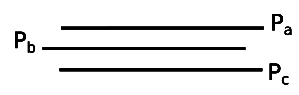
\includegraphics[width=4.5cm]{img/edge-clique.png} & &
    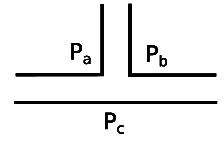
\includegraphics[width=3.5cm]{img/claw-clique.png}%b1EpgTransparenteGrade2
    \\
    \footnotesize %\centering 
    (a)  \footnotesize Representation of a clique as edge-clique. && \footnotesize (b) Representation  of a clique as claw-clique.\\
  \end{tabular}

 \caption{Examples of clique representations.} \label{fig:cliquesRepresentation}
\end{figure}


















% \begin{figure}[h]
%   \centering
%   \begin{tabular}{  p{4cm} p{0.7cm} p{4cm} }
%     %\centering
%     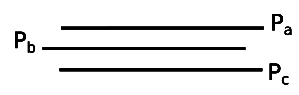
\includegraphics[width=4.5cm]{img/edge-clique.png} & &
%     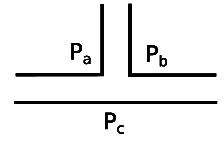
\includegraphics[width=3.5cm]{img/claw-clique.png}%b1EpgTransparenteGrade2
%     \\
%     \footnotesize %\centering 
%     (a)  \footnotesize Representação de uma  clique como clique-aresta. && \footnotesize (b) Representação de uma  clique como clique-garra.\\
%   \end{tabular}

%  \caption{Exemplos de representações de clique.} \label{fig:cliquesRepresentation}
% \end{figure}    

Notice that if three vertices induce a claw-clique, then exactly two of them turn at the center of the corresponding  claw of the grid, and the third one contains the
base of the claw. 
Furthermore, any other vertex  adjacent to the three  must contain two of the edges of that claw, then the following lemma holds.

\begin{lema}\label{lem:cliquesMaximais}
If three vertices are together  in more than one maximal clique of a graph $G$, then in
any $B_1$-EPG representation of $G$ the three vertices do not form a claw-clique. %corresponding paths do not form a claw.
\end{lema}

\begin{figure}[ht]
  \centering
  \begin{tabular}{  p{5cm} p{0.7cm} p{5cm} }
    %\centering
    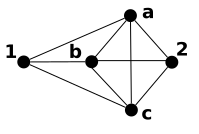
\includegraphics[width=3.5cm]{img/lemaClaw2Maximais} & &
    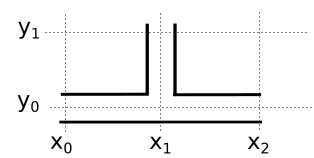
\includegraphics[width=5.5cm]{img/claw2}
    \\
    \footnotesize %\centering 
    (a)  \footnotesize Examplo de duas cliques maximais compartilhando vértices. && \footnotesize (b) Representação de uma clique-garra na grade.\\
  \end{tabular}

 \caption{Vértices representados por uma garra  estão presentes em uma única clique maximal.} \label{fig:lemaClaw2Maximais}
\end{figure}

In \cite{ries2009} Asinowski et al. proved the following lemma for $C_4$-free graphs.

\begin{lema} \cite{ries2009} \label{lem:lemaBRies2009}
Let $G$ be a $B_1$-EPG graph. If $G$ is $C_4$-free, then there exists a $B_1$-EPG representation of $G$ such that every  maximal claw-clique $K$ is represented on a claw of the grid whose base is covered only by vertices of $K$.
\end{lema}


We have obtained the following similar result for diamond-free graphs. A \textit{diamond} is a graph $G$ with vertex set $V(G) = \{a, b, c, d\}$ and edge set $E(G)=\{ab, ac,bc, bd,cd\}$ (see Figure~\ref{fig:diamond}). %A graph is diamond-free if it does not contain a diamond as induced subgraph.

 \begin{figure}[htb]	
 \center%6.3
 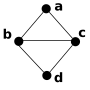
\includegraphics[width=2.2cm]{./img/diamond.png}
 \caption{Diamond graph.}
\label{fig:diamond}
\end{figure}  
 


\begin{lema}\label{lem:b1epgDiamondFree}
Let $G$ be a $B_1$-EPG graph. If $G$ is diamond-free, then in any $B_1$-EPG representation of $G$,  every maximal claw-clique $K$ is represented on a claw of the grid whose edges are covered only by vertices of $K$.
\end{lema}

% \begin{proof}Let $K$ be a maximal clique which is a claw-clique in a given $B_1$-EPG representation of $G$. Then there exist three vertices of $K$ which induce a claw-clique $K'$ on
% the same claw of the grid than $K$. Assume, in order to derive a contradiction, that a vertex $v\notin K$ covers some edge of the claw. Clearly, $v$ must  cover
% only one of such edges. Therefore $v$ and the vertices of $K'$ induce a diamond, a contradiction. 
% \end{proof}


Let $ Q $ be a grid and let $ (a_1, b),$ $(a_2, b),$ $(a_3, b),$ $(a_4, b)$ be a $4$-star centered at $b$ as depicted in Figure~\ref{fig:piesInGrid}(a). Let $ \mathcal{P} = \{P_1, \dots , P_4\}$ be a collection of four paths each containing a different pair of edges of the $4$-star.
%exactly two edges of the $4$-star:
Following \cite{golumbic2009}, we say that the four paths form
\begin{itemize}
\item a \emph{true pie} %is a representation where each $P_i$ of $ \mathcal{P} $ has a bend at $b$.
when each one has a bend at $b$, Figure~\ref{fig:piesInGrid}(b); and 
\item a \emph {false pie} when exactly two of the paths %$P_i$  do not 
bend at $b$ and they do not share an edge of the $4$-star, Figure~\ref{fig:piesInGrid}(c). %contain bends, while the remaining two do not share an edge. 

\begin{figure}[htb]
  \centering
%segundo bloco de figuras
  \begin{tabular}{c c c c c }
    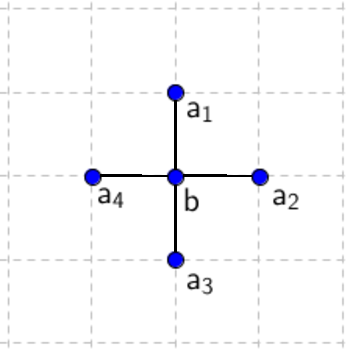
\includegraphics[width=3.5cm]{img/disposicaoTortaGrid3.pdf}    
    & &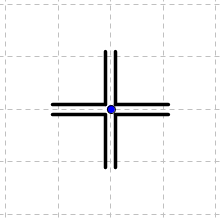
\includegraphics[width=3.5cm]{img/truePieGrid} 
    & &
 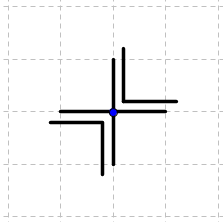
\includegraphics[width=3.5cm]{img/falsePieGrid} \\%[\abovecaptionskip]
    {\footnotesize (a) 4-estrela em uma grade.}  & &  {\footnotesize (b) Torta verdadeira.} & & {\footnotesize (c) Torta falsa.} 
  \end{tabular}
  \caption{Representação $B_{1}$-EPG do ciclo induzido de tamanho  4 como tortas, com ênfase no centro $b$.}\label{fig:piesInGrid}
\end{figure} 

%\vspace{-0.5cm}
\end{itemize}
% \end{defi}

Clearly if four paths of a $B_1$-EPG representation of $G$ form a pie, then the corresponding vertices induce a $4$-cycle in $G$. % The converse implication is also true (see~\cite{golumbic2009}). 
The following result can be easily proved. We say that a set of paths form a claw when each pair of edges of the claw is covered by some of the paths.

\begin{lema}\label{lem:twoClawNotSameCenterInChordal}
In any $B_1$-EPG representation of a graph $G$, a set of paths forming two different claws centered at the same point of the grid contains four paths forming either a true pie or a false pie. Therefore, in any $B_1$-EPG representation of a chordal graph $G$, no two maximal claw-cliques of $G$ are centered at the same point of the grid.
\end{lema}

\begin{lema}\label{lem:3cliquesNotClaw}
Let $G$ be a graph whose vertex set  can be
partitioned into a non trivial clique $K$ and an independent set $I=\{w_1,w_2,w_3\}$, such that each vertex of $K$ is adjacent to each vertex of $I$. Then, in any $B_1$-EPG representation of $G$, at least one of the cliques  $K_i = K \cup \{w_i\}$, with $1 \leq i \leq 3$,  is an edge-clique. 
\end{lema}

% \begin{proof}
% Assume, in order to derive a contradiction, that the three cliques are claw-cliques. By Lemma~\ref{lem:twoClawNotSameCenterInChordal}, they have different centers, say the points $q_1, q_2, q_3$ of the grid, respectively. Since at least two paths have a bend at the center of a claw, for each $i\in\{1,2,3\}$,   there must exist a vertex
%   $v_i$ of $K$ such that the corresponding path $P_{v_i}$ turns at the point $q_i$ of the grid.  Notice that each one of the three paths $P_{v_i}$
%   must contain  the three grid points $q_1$, $q_2$ and $q_3$. To prove that this is not possible, we will consider, without loss of generality, two cases.
%   First,  $q_1$ is between $q_2$ and $q_3$ in $P_{v_1}$. Then, $P_{v_3}$ cannot turn at $q_3$ and contain $q_1$ and $q_2$.   And second,
%   $q_2$ is between $q_1$ and $q_3$ in $P_{v_1}$. In this case, $P_{v_2}$ cannot turn at $q_2$ and contain $q_1$ and $q_3$; thus the proof is completed.
% \end{proof}

Three vertices $u, v, w$ of a graph $G$ form an \textit{asteroidal triple} (AT) of $G$ if for every pair of them there exists a path connecting the two vertices and such that the path avoids the neighborhood of the remaining vertex~\cite{Asinowski2009}. A graph without an asteroidal triple is called \textit{AT-free}. 

\begin{lema}
[\cite{ries2009}] \label{l:AT-free} Let $v$ be any vertex of a $B_1$-EPG graph $G$. Then $G[N(v)]$ is AT-free.
\end{lema}

Let $C$ be any subset of the vertices of a graph $G$. The \textit{branch graph} $B(G|C)$, see~\cite{golumbic2009}, of $G$ over $C$ has a vertex set, $V(B)$, consisting of all the vertices of $G$ not in $C$ but adjacent to some member of $C$, i.e. $V(B) = N(C) - C$. Adjacency in $B(G|C)$ is defined as follows: we join two vertices $x$ and $y$ by an edge in $E(B)$ if and only if in $G$ occurs:
\begin{enumerate}
    \item  $x$ and $y$ are not adjacent;
    \item $x$ and $y$ have a common neighbor $u \in C$;
    \item the sets $N(x) \cap C$ and $N(y) \cap C$ are not comparable, i.e. there exist private neighbors $w, z \in C$ such that $w$ is adjacent to $x$ but not to $y$, and $z$ is adjacent to $y$ but not to $x$; we say that $x$ and $y$ are neighborhood incomparable.
\end{enumerate}

A graph $G$ is \textit{k-colorable} if its vertices can be colored with at most $k$ colors in such a way that no two adjacent vertices share the same color. 

\begin{lema}[~\cite{golumbic2009}] \label{l:branch} Let $C$ be any maximal clique of a $B_1$-EPG  graph $G$. Then, the branch graph $B(G|C)$ is $\{P_6, \, C_n \hbox{ for }  n\geq 4\}$-free.
\end{lema}







\section{Subclasses of Helly-$B_1$-EPG Graphs}

In this section, we delimit some  subclasses of $B_1$-EPG graphs that admit a Helly-$B_1$-EPG representation. It is known that $B_1$-EPG and Helly-$B_1$ EPG 
are hereditary classes, so they can  be characterized by forbidden structures. 
In both cases, finding the list of minimal forbidden induced subgraphs are challenging open problems.
Taking a step towards solving
those problems,  we describe a few structures % that  provide a $B_1$-EPG graph does not admit a Helly-$B_1$ EPG representation, that is it is not a  Helly-$B_1$ EPG graph. 
at least one of which will  necessarily be present in  any $B_1$-EPG graph that does not admit a Helly representation. 
In addition,
we show that the well known families of Block graphs, Cactus and Line of Bipartite graphs are totally contained in the class Helly-$B_1$ EPG.


Let $S_{3}, S_{3'}, S_{3''}$ and $ C_{4}$ be the graphs depicted in Figure \ref{fig:proibidos}. 


\begin{theorem}
\label{lem:chordalDiamondFree}
Let $G$ be a $B_1$-EPG graph. If $G$ is  $\{S_{3}, S_{3'}, S_{3''}, C_{4}\}$-free then $G$  is a Helly-$B_1$-EPG graph.
\end{theorem}

% \begin{proof}
% If $G$ is not a Helly-$B_1$-EPG graph, then in each $B_1$-EPG representation of $G$, there is at least one clique that is represented as claw-clique and no as edge-clique. Consider any $B_1$-EPG  representation of $G$  and let $K$ be a maximal clique  which is represented as a claw-clique. Assume, w.l.o.g,  $K$ is on a claw of the grid with base $[x_0, x_2]\times\{y_0\}$ and center $C = (x_1, y_0)$. Denote by  $\mathcal{P}_K$ the set of paths corresponding to the vertices of $K$.  By Lemma~\ref{lem:lemaBRies2009},   
% the grid segment $[x_0, x_2]\times\{y_0\}$ is covered only by vertices of $K$. 


%  For every ${\displaystyle \lrcorner}$-path   
%  (resp. ${\displaystyle \llcorner}$-path) belonging to $\mathcal{P}_K$, we do the following: if 
%  the path does not intersect any path $P_t \notin\mathcal{P}_K$ on column $x_1$, then we delete its vertical segment and add the grid segment $[x_1, x_2]\times\{y_0\}$ (resp. $[x_0, x_1]\times\{y_0\}$). If after this transformation there is no more ${\displaystyle \lrcorner}$-paths (resp. ${\displaystyle \llcorner}$-paths) in $\mathcal{P}_K$, then we are done since we have obtained an edge-clique. So we may assume that
%  every ${\displaystyle \lrcorner}$-path   and every ${\displaystyle \llcorner}$-path  in $ \mathcal{P}_K$ intersects some path $P_t \notin \mathcal{P}_K$   on column $x_1$ (notice that we can assume is the same path $P_t$ for all the vertices). 
 
%  Now, if none of the ${\displaystyle \lrcorner}$-paths belonging to $\mathcal{P}_K$ intersects  a path non in  $ \mathcal{P}_K$ on the line $y_0$, then we can replace the horizontal part of those paths by the segment $[x_1,x_2]\times \{y_0\}$, getting an edge representation of the clique $K$. Thus, we can assume there exists
%  at least one ${\displaystyle \lrcorner}$-path $P_{v} \in \mathcal{P}_K$ intersecting some path  $P_{t'} \notin \mathcal{P}_K$ on line $y_0$. Analogously, there exists
%  at least one ${\displaystyle \llcorner}$-path $P_{v'} \in \mathcal{P}_K$ intersecting some path  $P_{t''} \notin K$ on line $y_0$, as depicted in Figure~\ref{fig:clawGrid}. Notice that vertex $t'$ cannot be adjacent to any of the vertices $t$, $v'$ or $t''$; and, in addition, vertex $t''$ cannot
%  be adjacent to   $t$,  or $v$.
 
%  Finally,   since $K$ is claw-clique,  there is a path $P_u \in \mathcal{P}_K$ covering the base of the claw. Depending on the 
%  possibles adjacencies between  $u$ and $t'$ or  $t''$, one of the graphs  $S_{3}$, $S_{3'}$ or $S_{3''}$ is obtained.
% \end{proof}

The proof of previously theorem is based on the idea of that the set of graphs mentioned form claw-cliques that can not be transformed into edge-cliques. 



\begin{figure}[h]
  \centering
  \begin{tabular}{  c p{0.7cm} c}
    %\centering
    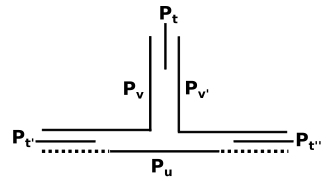
\includegraphics[width=5.5cm]{img/clawGrid} & &
    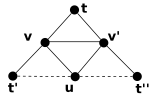
\includegraphics[width=3.5cm]{img/clawInduced.png}
    \\
    \footnotesize %\centering 
    (a)  \footnotesize Claw with paths. && \footnotesize (b) Subgraph induced by paths.\\
  \end{tabular}

 \caption{Reconstruction of the intersection model.}
 \label{fig:clawGrid}
\end{figure} 

 


% \begin{figure}[h]
%   \centering
%   \begin{tabular}{  c p{0.7cm} c}
%     %\centering
%     \includegraphics[width=5.5cm]{img/clawGrid} & &
%     \includegraphics[width=3.5cm]{img/clawInduced.png}
%     \\
%     \footnotesize %\centering 
%     (a)  \footnotesize Clique-garra com caminhos adicionais. && \footnotesize (b) Subgrafo induzido pelos caminhos.\\
%   \end{tabular}

%  \caption{Reconstrução do modelo de intersecção.}
%  \label{fig:clawGrid}
% \end{figure} 

 



Notice that any bull-free graph is $\{S_{3}, S_{3'}, S_{3''}\}$-free, so our previous result implies  Lemma 5 of  \cite{ries2009}.


\begin{figure}[h]
  \centering
  \begin{tabular}{  c p{0.7cm} c }
    \centering
    \includegraphics[width=4cm]{img/s3.png} & &
    \includegraphics[width=4cm]{img/s3-1.png}
    \\
    \footnotesize \centering 
    (a)  \footnotesize Grafo $S_3$. &&  \footnotesize (b) Grafo $S_{3'}$. \\
    
    %---------------------
      \centering 
      \includegraphics[width=4cm]{img/s3-2.png} & &
    \includegraphics[width=3cm]{img/c4.png}
    \\
    \footnotesize \centering 
    (c)  \footnotesize Grafo $S_{3''}$. && \footnotesize (b) Grafo $C_{4}$.\\
  \end{tabular}

 \caption{Grafos do enunciado do  Teorema~\ref{lem:chordalDiamondFree}.}
 \label{fig:proibidos}
\end{figure} 



%--------------------------


Next theorem has as consequence the identification of several graph classes where the existence of a $B_1$-EPG representation ensures the existence of a Helly-$B_1$-EPG representation.


\begin{theorem} \label{lem:b1DiamondFree}
 If $G$ is a $B_1$-EPG and diamond-free graph then $G$ is a Helly-$B_1$-EPG graph.
 \end{theorem}

% \begin{proof}
% If $G$ is not a Helly-$B_1$-EPG graph, then in each $B_1$-EPG representation of $G$, there is at least one clique that is represented as claw-clique and no as edge-clique.  Consider any $B_1$-EPG  representation of $G$  and let $K$ be a maximal clique  which is represented as a claw-clique. Assume, w.l.o.g,  $K$ is on a claw of the grid with base $[x_0, x_2]\times\{y_0\}$ and center $C = (x_1, y_0)$. Denote by  $\mathcal{P}_K$ the set of paths corresponding to the vertices of $K$. 
%  By Lemma~\ref{lem:b1epgDiamondFree},   
% the grid segment $[x_0, x_2]\times\{y_0\}$ is covered only by vertices of $K$.  
%  For every ${\displaystyle \lrcorner}$-path  
%  (resp. ${\displaystyle \llcorner}$-path) belonging to $\mathcal{P}_K$, we do the following: if  
%  the path does not intersect any path $P_t \notin\mathcal{P}_K$ on column $x_1$, then we delete its vertical segment and add the grid segment $[x_1, x_2]\times\{y_0\}$ (resp. $[x_0, x_1]\times\{y_0\}$). If after this transformation there is no more ${\displaystyle \lrcorner}$-paths (resp. ${\displaystyle \llcorner}$-paths) in $\mathcal{P}_K$, then we are done since we have obtained an edge-clique. So we may assume that
%  every ${\displaystyle \lrcorner}$-path   and every ${\displaystyle \llcorner}$-path  in $ \mathcal{P}_K$ intersects some path $P_t \notin \mathcal{P}_K$   on column $x_1$ (notice that we can assume is the same path $P_t$ for all the vertices). Since  $K$ is claw-clique,  there is a path $P_u \in \mathcal{P}_K$ covering the base of the claw. Thus, $G[v, v', u, t]$ induces a diamond,  a contradiction. 
% \end{proof}  

An \textit{independent set} of vertices is a set of vertices no two of which are adjacent.
A graph $G$ is said to be \textit{Bipartite} if its set of vertices can be partitioned into two distinct independent sets.
 There are Bipartite graphs that are non $B_1$-EPG, for instance $K_{2,5}$ and $K_{3,3}$ (see~\cite{cohen2014}). Clearly , since
 bipartite graphs are triangle-free, any $B_1$-EPG representation of a bipartite graph is also a Helly-$B_1$-EPG representation.
 A similar result (but a bit weaker) is obtained as corollary of the previous theorem. 


\begin{corollary}
If $G$ is a Bipartite $B_1$-EPG graph then $G$ is a Helly-$B_1$-EPG graph.
\end{corollary}

% \begin{proof}
% The Bipartite graphs are diamond-free, thus by Theorem~\ref{lem:b1DiamondFree} these graphs are Helly-$B_1$-EPG graphs.
% \end{proof}

A \textit{Block graph} or \textit{Clique Tree} is a type of graph in which every biconnected component (block) is a clique.

\begin{corollary}\label{lem:cdf}
 Block graphs are Helly-$B_1$ EPG.
\end{corollary}

% \begin{proof}
% Block graphs are known to be exactly the chordal diamond-free graphs, so by   Theorem 19 of \cite{ries2009}, all Block graphs are  $B_1$-EPG. If follows from Theorem~\ref{lem:b1DiamondFree} that all Block graphs are Helly-$B_1$ EPG. 
%  \end{proof} 

A \textit{Cactus} (sometimes called a Cactus Tree)  graph is a connected graph in which any two  cycles have at most one vertex in common. Equivalently, it is a connected graph in which every edge belongs to at most one  cycle, or (for nontrivial Cactus) in which every block (maximal subgraph without a cut-vertex) is an edge or a cycle. The family of graphs in which each component is a Cactus is closed under graph minor operations. This graph family may be characterized by a single forbidden minor, the diamond graph.
 
\begin{corollary}
Cactus graphs are  Helly-$B_1$ EPG.
\end{corollary}
% \begin{proof}
% In~\cite{cela2019monotonic}, it is proved that every Cactus graph is a monotonic $B_1$-EPG graph 
% (there is a $B_1$-EPG representation where all paths are ascending in rows and columns). 
% Thus, Cactus graphs are $B_1$-EPG graphs. 

% Since Cactus are diamond-free, by Theorem ~\ref{lem:b1DiamondFree}, the proof follows.
% \end{proof}

Given a graph $G$, its \textit{Line graph} $L(G)$ is a graph such that each vertex of $L(G)$ represents an edge of $G$ and
  two vertices of $L(G)$ are adjacent if and only if their corresponding edges share a common endpoint (i.e. ``are incident'') in $G$.  
A graph $G$ is a \textit{Line graph of a Bipartite graph} (or simply \textit{Line of Bipartite}) if and only if it
contains no claw, no odd cycle  (with more than three vertices), and no diamond as induced subgraph, \cite{harary1974line}.

In~\cite{daniel2014b} was proved that every Line graph has a representation with at most 2 bends. We proved in the follow corollary that when restricted to the Line of Bipartite we can obtain a representation Helly and one-bended.

\begin{corollary}\label{coro:lineOfBipartite}
 Line of Bipartite graphs are Helly-$B_1$ EPG. 
\end{corollary}

% \begin{proof}
% Line of Bipartite graphs were proved to be $B_1$-EPG in~\cite{golumbic2018edge}. Since they are diamond-free, the proof follows from Theorem~\ref{lem:b1DiamondFree}.
% \end{proof}

The diagram of Figure~\ref{fig:diagram}
illustrates the containment relationship between the graph classes  studied so far in this work. 
We list in Figure~\ref{fig:exemplosDiagram} examples of graphs in each numbered region of the diagram. The numbers of each item below correspond to the regions of the same number in the diagram depicted in Figure~\ref{fig:diagram}.

%This numbers correspond with the respective number item and in some cases we make a brief explanation.

% \begin{enumerate}[label=(\arabic*)]
%     \item $B_1$-EPG  - Helly-$B_1$-EPG graphs, depicted in Figure~\ref{fig:exemplosDiagram}(a), graph $E_1$;%1
    
%     \item Line of Bipartite graphs  - Cactus - Block - Bipartite graphs, depicted in Figure~\ref{fig:exemplosDiagram}(b), graph $E_2$;%2
%     \item Helly-$B_1$ EPG - Line of Bipartite - Block - Cactus - Bipartite graphs, depicted in Figure~\ref{fig:exemplosDiagram}(c), graph $E_3$;%3
%     \item Block $\cap$ Line of Bipartite - Cactus - Bipartite, depicted in Figure~\ref{fig:exemplosDiagram}(d), graph $E_4$;%4
%     \item Block $\cap$ Line of Bipartite $\cap$  Cactus - Bipartite, depicted in Figure~\ref{fig:exemplosDiagram}(e), graph $E_5$;%5
%     \item Cactus $\cap$ Line of Bipartite - Block - Bipartite. This intersection is empty. Let $G$ be a graph that is Cactus and Line of Bipartite then $G$ is $\{$claw, odd cycle, diamond$\}$-free. But $G$ is not a Bipartite graph, then $G$ has odd cycle, %. Thus $G$ has at least one triangle or at least one odd cycle $C_n, n\geq 4$, and $G$ is a connected graph. But given a cycle $C_n, n\geq 4$, if add one vertex any adjacent to this cycle then this induce a claw, 
%      absurd with the hypothesis of $G$ is Line of Bipartite;%6
%     \item Bipartite $\cap$ Line of Bipartite  - Cactus - Block graphs, depicted in Figure~\ref{fig:exemplosDiagram}(f), graph $E_7$;%7
%     \item Bipartite $\cap$ Line of Bipartite $\cap$  Cactus - Block graphs, depicted in Figure~\ref{fig:exemplosDiagram}(g), graph $E_8$;%8
%     \item Bipartite $\cap$ Line of Bipartite $\cap$  Cactus $\cap$ Block graphs, depicted in Figure~\ref{fig:exemplosDiagram}(h), graph $E_9$;%9
%   \item Bipartite $\cap$  Cactus $\cap$ Block - Line of Bipartite graphs, depicted in Figure~\ref{fig:exemplosDiagram}(i), graph $E_{10}$;%10
%     \item Bipartite  $\cap$  Cactus - Block -  Line of Bipartite graphs, depicted in Figure~\ref{fig:exemplosDiagram}(j), graph $E_{11}$;%11
%      \item Bipartite $\cap$ Helly-$B_1$ EPG - Cactus - Block -  Line of Bipartite graphs, depicted in Figure~\ref{fig:exemplosDiagram}(k), graph $E_{12}$;%12
%       \item Bipartite - $B_1$-EPG graphs, depicted in Figure~\ref{fig:exemplosDiagram}(l), graph $E_{13}$;%13
%       \item Block - Bipartite - Line of Bipartite  - Cactus graphs, depicted in Figure~\ref{fig:exemplosDiagram}(m), graph $E_{14}$;%14
 
%       \item Block $\cap$  Cactus -  Line of Bipartite - Bipartite graphs, depicted in Figure~\ref{fig:exemplosDiagram}(n), graph $E_{15}$;%15
%       \item Cactus - Block -  Line of Bipartite - Bipartite graphs, depicted in Figure~\ref{fig:exemplosDiagram}(o), graph $E_{16}$, the odd cycles $C_{2n+1},n\geq 2$;%16
%       \item Helly EPG - $B_1$-EPG  - Bipartite graphs, depicted in Figure~\ref{fig:exemplosDiagram}(p), graph  $E_{17}$;%17
% \end{enumerate}

\begin{enumerate}[label=(\arabic*)]
    \item ($B_1$-EPG)  - (Helly-$B_1$-EPG) graphs, depicted in Figure~\ref{fig:exemplosDiagram}(a), graph $E_1$. In~\cite{bornstein2019,dmtcs:6506} was proved that the octahedral graph does not belong to Helly-$B_1$ EPG despite belonging to $B_1$-EPG;%1
    
    \item (Line of Bipartite)  - (Cactus) - (Block) - (Bipartite) graphs, depicted in Figure~\ref{fig:exemplosDiagram}(b), graph $E_2$. The graph $E_2$ contains no claw, no odd cycle, and no diamond as induced subgraph, therefore it is Line of Bipartite. But $E_2$ has two cycles sharing two vertices, thus it is not a Cactus graph. There is  in $E_2$ a biconnected component that is not a clique, then the graph $E_2$ is not a Block graph. Finally, $E_2$ also  has three vertices pairwise intersecting, thus it is not a Bipartite graph;%2
    \item (Helly-$B_1$ EPG) - (Line of Bipartite) - (Block) - (Cactus) - (Bipartite) graphs, depicted in Figure~\ref{fig:exemplosDiagram}(c), graph $E_3$. It is easy to see that the graph $E_3$ is in Helly-$B_1$ EPG, but $E_3$ is a  diamond graph, therefore it is not Line of Bipartite, Block, Cactus nor Bipartite;%3
    \item (Block) $\cap$ (Line of Bipartite) - (Cactus) - (Bipartite), depicted in Figure~\ref{fig:exemplosDiagram}(d), graph $E_4$. The graph $E_4$ is a complete graph with four vertices, therefore is in (Block) $\cap$ (Line of Bipartite), but it is not in Cactus or Bipartite class;%4
    \item (Block) $\cap$ (Line of Bipartite) $\cap$  (Cactus) - (Bipartite), depicted in Figure~\ref{fig:exemplosDiagram}(e), graph $E_5$. The graph $E_5$ is both, a complete graph and a cycle of size 3, then it is in (Block) $\cap$ (Line of Bipartite) $\cap$  (Cactus) but it is not a Bipartite graph; %5
    \item (Cactus) $\cap$ (Line of Bipartite) - (Block) - (Bipartite). This intersection is empty. Let $G$ be a graph that is Cactus and Line of Bipartite then $G$ is $\{$claw, odd cycle, diamond$\}$-free. But $G$ is not a Bipartite graph, then $G$ has odd cycle, %. Thus $G$ has at least one triangle or at least one odd cycle $C_n, n\geq 4$, and $G$ is a connected graph. But given a cycle $C_n, n\geq 4$, if add one vertex any adjacent to this cycle then this induce a claw, 
     absurd with the hypothesis of $G$ is Line of Bipartite;%6
    \item (Bipartite) $\cap$ (Line of Bipartite)  - (Cactus) - (Block) graphs, depicted in Figure~\ref{fig:exemplosDiagram}(f), graph $E_7$. The graph $E_7$ is composite by two cycles of size 4, so it is in (Bipartite) $\cap$ (Line of Bipartite), but on the other hand how $E_7$ is not a connected graph then it is not Cactus or Block graph;%7
    \item (Bipartite) $\cap$ (Line of Bipartite) $\cap$  (Cactus) - (Block) graphs, depicted in Figure~\ref{fig:exemplosDiagram}(g), graph $E_8$. The graph $E_8$ is a cycle of size 4, so it is in (Bipartite) $\cap$ (Line of Bipartite) $\cap$  (Cactus), but on the other hand it is not a Block graph because there is a biconnected component that is not a clique;%8
    \item (Bipartite) $\cap$ (Line of Bipartite) $\cap$  (Cactus) $\cap$ (Block) graphs, depicted in Figure~\ref{fig:exemplosDiagram}(h), graph $E_9$;%9
  \item (Bipartite) $\cap$  (Cactus) $\cap$ (Block) - (Line of Bipartite) graphs, depicted in Figure~\ref{fig:exemplosDiagram}(i), graph $E_{10}$. The graph $E_{10}$ is a claw, therefore is in (Bipartite) $\cap$  (Cactus) $\cap$ (Block) but it is not in Line of Bipartite;%10
    \item (Bipartite)  $\cap$  (Cactus) - (Block) -  (Line of Bipartite) graphs, depicted in Figure~\ref{fig:exemplosDiagram}(j), graph $E_{11}$. The graph $E_{11}$ has no odd cycle and each biconnected component is a cycle then it is in (Bipartite)  $\cap$  (Cactus) and it is not a Block graph. Moreover, the graph $E_{11}$ has claw as induced subgraph, thus it is not Line of Bipartite graph;%11
     \item (Bipartite) $\cap$ (Helly-$B_1$ EPG) - (Cactus) - (Block) -  (Line of Bipartite) graphs, depicted in Figure~\ref{fig:exemplosDiagram}(k), graph $E_{12}$. It is easy to see that the graph $E_{12}$ is in (Bipartite) $\cap$ (Helly-$B_1$ EPG). There are two cycles sharing two vertices in $E_{12}$, thus it is not a Cactus graph. Moreover, the graph $E_{12}$ has a biconnected component that is not a clique then it is not a Block graph. Finally, the graph $E_{12}$ has a claw as induced subgraph, thus it is not a Line of Bipartite graph;%12
      \item (Bipartite) - ($B_1$-EPG) graphs, depicted in Figure~\ref{fig:exemplosDiagram}(l), graph $E_{13}$. In \citeauthor{cohen2014} \cite{cohen2014} was proved that the graph $K_{2,5}$ is not a $B_1$-EPG graph. The graph $E_{13}$ corresponds exactly to the $K_{2,5}$ graph, thus it is Bipartite graph that does not belong to $B_1$-EPG;%13
      \item (Block) - (Bipartite) - (Line of Bipartite)  - (Cactus) graphs, depicted in Figure~\ref{fig:exemplosDiagram}(m), graph $E_{14}$. It is easy to see that the graph $E_{14}$ is a Block graph. Since there is a biconnected component that is a complete graph with four vertices then $E_{14}$ is not a Bipartite graph nor a Cactus graph. Moreover $E_{14}$ has a claw as induced subgraph, thus it is not a Line of Bipartite graph;%14
 
      \item (Block) $\cap$  (Cactus) -  (Line of Bipartite) - (Bipartite) graphs, depicted in Figure~\ref{fig:exemplosDiagram}(n), graph $E_{15}$. It is easy to see that the graph $E_{15}$ is both Block and Cactus graph, but it has a cycle of size three and a claw as induced subgraph, thus this graph is not Line of Bipartite nor Bipartite;%15
      \item (Cactus) - (Block) -  (Line of Bipartite) - (Bipartite) graphs, depicted in Figure~\ref{fig:exemplosDiagram}(o), graph $E_{16}$, the odd cycles $C_{2n+1},n\geq 2$. Odd cycles are Cactus. The graph $E_{16}$ is a odd cycle then it is a Cactus graph but it is not a Block, Line of Bipartite or Bipartite graph;%16
      \item (Helly EPG) - ($B_1$-EPG)  - (Bipartite) graphs, depicted in Figure~\ref{fig:exemplosDiagram}(p), graph  $E_{17}$. In \citeauthor{golumbic2009} \cite{golumbic2009} has been proved that the graph $k$-sun for $k\geq 4$ is not a $B_1$-EPG graph. The graph $E_{17}$ is isomorphic to $4$-sun, thus it is not a  $B_1$-EPG but it is Helly-EPG because all graphs are Helly-EPG for some $k$ in a Helly-$B_k$-EPG representation, see
     ~\cite{dmtcs:6506};%17
\end{enumerate}


 \begin{figure}[htb]	
 \center%6.3
 \includegraphics[width=8cm]{./img/diagram.pdf}
 \caption{Diagrama de algumas classes de grafos.}
\label{fig:diagram}
\end{figure}  
 


 \begin{figure}[htb]	
 
   \centering
  \begin{tabular}{  c c c c  c}
    %\centering
    \includegraphics[width=2cm]{img/octaedroNoLabel.png} 
    & 
    \includegraphics[width=1.5cm]{img/ex3.png} 
    & 
    \includegraphics[width=2cm]{img/diamondNoLabel.png} 
    & 
    \includegraphics[width=1.5cm]{img/k4.png} 
    & 
    \includegraphics[width=2cm]{img/k3.png} 
    \\
    \footnotesize 
    (a)  \footnotesize Graph $E_1$. 
    & 
    \footnotesize (b) Graph $E_2$.
    & 
    \footnotesize (c) Graph $E_3$.
    & 
    \footnotesize (d) Graph $E_4$.
    & 
    \footnotesize (e) Graph $E_5$.
    \\%%Segunda linha
        \includegraphics[width=2.5cm]{img/2c4.png} 
    & 
    \includegraphics[width=1.5cm]{img/c4e.png} 
    & 
    \includegraphics[width=1.8cm]{img/k2.png} 
    & 
    \includegraphics[width=1cm]{img/e10.png} 
    & 
    \includegraphics[width=1.8cm]{img/e11.png} 
    \\ %%Segundo Bloco legendas
    \footnotesize 
    (f)  \footnotesize Graph $E_7$. 
    & 
    \footnotesize (g) Graph $E_8$.
    & 
    \footnotesize (h) Graph $E_9$.
    & 
    \footnotesize (i) Graph $E_{10}$.
    & 
    \footnotesize (j) Graph $E_{11}$.
    %%Terceira linha de imagens
    \\%%Terceira linha
        \includegraphics[width=2.5cm]{img/e12.png} 
    & 
    \includegraphics[width=2cm]{img/k25.png} 
    & 
    \includegraphics[width=2cm]{img/e14.png} 
    & 
    \includegraphics[width=1.8cm]{img/e15.png} 
    & 
    \includegraphics[width=1.8cm]{img/c2n+1.png} 
    \\ %%Terceiro Bloco legendas
    \footnotesize 
    (k)  \footnotesize Graph $E_{12}$. 
    & 
    \footnotesize (l) Graph $E_{13}$.
    & 
    \footnotesize (m) Graph  $E_{14}$.
    & 
    \footnotesize (n) Graph $E_{15}$.
    & 
    \footnotesize (o)  Graph $E_{16}$,  $C_{2n+1},n\geq2$.
    \\
    &&\includegraphics[width=2.5cm]{img/4sunNoLabel.png}&&
    \\
    &&\footnotesize (p)  Graph $E_{17}$.&&
    
    %\multicolumn{3}{c}{ \footnotesize (c) Another partial single bend representation of $H$ } \\
  \end{tabular}
 \caption{The set of instances for Venn Diagram of the graph classes of this paper.}
 %, see  more in~\cite{leveque2009characterizing,tondato2009grafos}
 \label{fig:exemplosDiagram}
\end{figure}  
 



















%  \begin{figure}[htb]	
 
%   \centering
%   \begin{tabular}{  c c c c  c}
%     %\centering
%     \includegraphics[width=1.7cm]{img/octaedro2.png} 
%     & 
%     \includegraphics[width=1.5cm]{img/ex3.png} 
%     & 
%     \includegraphics[width=2cm]{img/diamondNoLabel.png} 
%     & 
%     \includegraphics[width=1.5cm]{img/k4.png} 
%     & 
%     \includegraphics[width=2cm]{img/k3.png} 
%     \\
%     \footnotesize 
%     (a)  \footnotesize Grafo $E_1$. 
%     & 
%     \footnotesize (b) Grafo $E_2$.
%     & 
%     \footnotesize (c) Grafo $E_3$.
%     & 
%     \footnotesize (d) Grafo $E_4$.
%     & 
%     \footnotesize (e) Grafo $E_5$.
%     \\%%Segunda linha
%         \includegraphics[width=2.5cm]{img/2c4.png} 
%     & 
%     \includegraphics[width=1.5cm]{img/c4e.png} 
%     & 
%     \includegraphics[width=1.8cm]{img/k2.png} 
%     & 
%     \includegraphics[width=1cm]{img/e10.png} 
%     & 
%     \includegraphics[width=1.8cm]{img/e11.png} 
%     \\ %%Segundo Bloco legendas
%     \footnotesize 
%     (f)  \footnotesize Grafo $E_7$. 
%     & 
%     \footnotesize (g) Grafo $E_8$.
%     & 
%     \footnotesize (h) Grafo $E_9$.
%     & 
%     \footnotesize (i) Grafo $E_{10}$.
%     & 
%     \footnotesize (j) Grafo $E_{11}$.
%     %%Terceira linha de imagens
%     \\%%Terceira linha
%         \includegraphics[width=2.5cm]{img/e12.png} 
%     & 
%     \includegraphics[width=2cm]{img/k25.png} 
%     & 
%     \includegraphics[width=2cm]{img/e14.png} 
%     & 
%     \includegraphics[width=1.8cm]{img/e15.png} 
%     & 
%     \includegraphics[width=1.8cm]{img/c2n+1.png} 
%     \\ %%Terceiro Bloco legendas
%     \footnotesize 
%     (k)  \footnotesize Grafo $E_{12}$. 
%     & 
%     \footnotesize (l) Grafo $E_{13}$.
%     & 
%     \footnotesize (m) Grafo  $E_{14}$.
%     & 
%     \footnotesize (n) Grafo $E_{15}$.
%     & 
%     \footnotesize (o)  Grafo $E_{16}$,  $C_{2n+1},n\geq2$.
%     \\
%     &&\includegraphics[width=2.5cm]{img/4sunNoLabel.png}&&
%     \\
%     &&\footnotesize (p)  Grafo $E_{17}$.&&
    
%     %\multicolumn{3}{c}{ \footnotesize (c) Another partial single bend representation of $H$ } \\
%   \end{tabular}
%  \caption{O conjunto de instâncias para o diagrama de Venn das classes de grafos estudadas até aqui.}
%  %, see  more in~\cite{leveque2009characterizing,tondato2009grafos}
%  \label{fig:exemplosDiagram}
% \end{figure}  
 

In next section we explore the Chordal $B_1$-EPG graphs through of a subset of forbidden graphs and we will proof that this class is in the strict intersection of VPT and EPT graphs.

\section{Containment relationship among Chordal $B_1$-EPG, VPT and EPT graphs }


 Any graph that
admits a $B_1$-EPG representation  whose paths do not cover all the edges of a polygon of the grid (i.e.
the subjacent grid subgraph is a tree)  is also an EPT graph: the same representation is both $B_1$-EPG and $EPT$.
However, it is easily verifiable that the subjacent grid subgraph of any $B_1$-EPG representation of a cycle $C_n$ with $n\geq 5$ is not a tree,
%has a non chordal subjacent grid subgraph 
although $C_n$ is an  EPT graph.  Our long-rage goal is 
understanding the $B_1$-EPG graphs that are also EPT graphs. When can a $B_1$-EPG representation
be reorganized into an EPT representation?  In this section,
 we answer that question for Chordal $B_1$-EPG graphs, in fact we prove that every Chordal $B_1$-EPG graph is EPT. We
 made several unsuccessful attempts to prove this result by considering for a graph $G$, a $B_1$-EPG representation whose paths cover all the edges
 of some polygon on the grid, and trying  to show  that if none of the paths could be modified in order to avoid an edge of the polygon,
 then $G$ had some chordless  cycle (i.e. $G$ is not Chordal). The surprise was that the only way we found to demonstrate our main Theorem \ref{teo:b1epgept} was through $VPT$ graphs.
 We will prove the following theorem.

\begin{theorem}\label{teo:chordalB1inVPT}
Chordal $B_1$-EPG $\subsetneq$ VPT. 
\end{theorem}

In~L{\'e}v{\^e}que et al. \cite{leveque2009characterizing} apud \cite{alcon2015characterizing},  VPT graphs were characterized by a family of minimal forbidden induced subgraphs,
the ones depicted in 
Figure~\ref{fig:16proibidos} plus the induced cycles $C_n$ for $n\geq 4$. Therefore, in order to prove
that Chordal $B_1$-EPG graphs are VPT is enough to show that none of the graphs in Figure~\ref{fig:16proibidos} 
is $B_1$-EPG. %The following lemmas are developed with that objective.   

First notice that in each one of the graphs $F_{1}, F_{2}, F_{3}, F_{4}$ and $F_{5}$ ( Figures~\ref{fig:16proibidos}(a), (b), (c), (d), (e), respectively), the neighborhood of the universal vertex (the one that is a bit bigger than the others, in the respective figures) contains an asteroidal triple. Therefore, by Lemma \ref{l:AT-free}, these graphs are not  $B_1$-EPG.

Now, in each one of the graphs $F_{11}, F_{12}, F_{13}, F_{14}$, $F_{15}$ and $F_{16}$  (Figures~\ref{fig:16proibidos}(k), (l), (m), (n), (o), (p), respectively), let $C$ be the maximal clique in bold. It is easy to check that, in all cases, the branch graph $B(G|C)$ contains an induced cycle $C_n$, for some $n\geq 4$, or an induced path $P_6$; thus, by Lemma \ref{l:branch},  graphs $F_{11}, F_{12}, F_{13}, F_{14}$, $F_{15}$ and $F_{16}$ are not $B_1$-EPG.



 % A \textit{satellite} of a clique $K$ is a vertex $v$ such that $B_v=N(v)\cap K$ is a 
%nonempty proper subset of $K$. The set $B_v$ is called the \textit{base} of $v$ and it is said \textit{minimal} if no other
%base of a satellite of $K$ is properly contained in $B_v$, see~\cite{alcon2010necessary}.

 %Let $I=[q_1,q_2]$ be the grid interval defined by the intersection $\displaystyle \cap_{v\in K}P_v$, where $K$
%is an edge-clique of a graph $G$. For any $v\in K$, by removing the interval $(q_1,q_2)$, the path $P_v$
%is split into two \textit{disjoint parts}: \textit{part 1}  containing $q_1$, and  \textit{part 2}  containing $q_2$.
%If $w$  is a satellite of $K$ adjacent to $v$, then
%$P_w\cap P_v$ is contained either in part 1 or in part 2 of $P_v$. We will say that $P_w$ intersects $P_v$
%on side 1 or on side 2 of $K$, respectively. Notice that if $w$  is also adjacent
%to another vertex $v'$ of $K$, then   $P_w$ intersects $P_v$ and $P_{v'}$ on
%a same side of $K$. It allow us to divide the satellites of $K$ into two \textit{disjoint
%groups}, the ones on  \textit{side 1} of $K$ and the ones on \textit{side 2}.

%%%%%%%%%%%%%%%%%%%%%%%%%%%
\begin{fac} \label{f:between}Let $e_{\ell}$, $e_m$ and $e_r$  be three distinct edges of a  one-bend path $P$, and assume that $e_m$ is between $e_{\ell}$ and $e_r$ on $P$. If $P_{\ell}$ and $P_r$ are one-bend paths such that: $P_{\ell}$ contains $e_{\ell}$, $P_r$ contains $e_r$, and  $P_{\ell}$ and $P_r$ intersect in at least one edge, then $P_{\ell}$ or $P_r$ contains $e_m$.
\end{fac}
%%%%%%%%%%%%%%%%%%%%%%%%%%%%%%
\begin{fac} \label{f:two points} Let  $e$ and $q$  be an edge and a  point  of a  one-bend path $P$, respectively. If a one-bend path $P'$ contains both $e$ and $q$, then $P'$ contains the whole segment of $P$ between $q$ and $e$.
\end{fac}

\begin{lema}\label{l:abclique}
Let $G$ be a graph whose vertex set  can be partitioned into a clique $K=\{a,b\}$ and an independent set $I=\{x,y,z\}$, such that each vertex of $K$ is adjacent to each vertex of $I$.
If in a given $B_1$-EPG representation of $G$, $P_a\cap P_y$ is between $P_a\cap P_x$ and $P_a\cap P_z$, then $\{a,b,y\}$ is an edge-clique, and
$P_a\cap P_y \subset P_b$. Even more, any vertex adjacent to $a$ and $y$, but not to $b$ (or to $b$ and $y$, but not to $a$) has to be adjacent to $x$ or to $z$.
\end{lema}

% \begin{proof}
% %%%%%%%%%%%%%%%%%%%%%%%%%%%%%%%
% Assume in order to obtain a contradiction that $\{a,b,y\}$ is not an edge-clique. Then, by Lemma
% \ref{lem:3cliquesNotClaw}, we can assume, w.l.o.g., that $\{a,b,x\}$ is an edge-clique.
% It implies that there is an edge $e_{\ell}$ of $P_a \cap P_x$ covered by $P_b$. Since every  edge
% of $P_a\cap P_z$ is covered  by $P_z$, $z$ and $b$ are adjacent, and $z$ and $y$ are non adjacent, we have by Fact \ref{f:between},
% that every edge of $P_a\cap P_y$ is covered by $P_b$, which implies  that $\{a,b,y\}$ is an edge-clique, contrary to the assumption.

% Thus, $\{a,b,y\}$ is an edge-clique. By Fact \ref{f:two points}, we have that the whole interval of $P_a$ between 
%  $P_a \cap P_x$ and   $P_a \cap P_z$ is contained in $P_b$, and so, in particular, $P_a\cap P_y \subset P_b$. Observe that this
%  implies that if $q$ is an end vertex of the interval $P_a \cap P_y$, and $e$ is the edge of $P_a$ incident on $q$ that do not belong to $P_y$, then 
% $e$ belongs to $P_b$ or to $P_x$ or to $P_z$.
 
%  Now, assume there exists a vertex $v$ adjacent to both $a$ and $y$ but not to $b$. Then, the clique $\{a,y,v\}$ has to be a claw-clique. Let $q$ be the center of the claw, notice that $q$ has to be an end vertex of the interval $P_a \cap P_y$.
%  Since $v$ is not adjacent to $b$, it follows from the observation at the end of the paragraph above, that
%  $v$ has to be adjacent to $x$ or to $z$.
% \end{proof}

\begin{lema}\label{lem:F_6}
The graph $F_6$ on Figure~\ref{fig:16proibidos}(f) is not   $B_1$-EPG.
\end{lema}
% \begin{proof} Let $K=\{1,2\}$ and $I=\{3,4,5\}$. If there exists a $B_1$-EPG representation of $F_6$,  by Lemma \ref{l:abclique},  because of the existence of the vertices $6$, $7$ and $8$, none of the vertices $3$, $4$ and $5$
% may intersect $1$ between the remaining two, thus such a representation does not exist.
%  \end{proof} 


\begin{lema}\label{lem:F_7}
The graph $F_7$ on Figure~\ref{fig:16proibidos}(g) is not   $B_1$-EPG.
\end{lema}
% \begin{proof} Let $K=\{1,2\}$ and $I=\{4,5,6\}$. If there exists a $B_1$-EPG representation of $F_7$,  by Lemma \ref{l:abclique},  because of the existence of the vertices  $7$ and $8$, the vertex $6$ must intersect  vertex $1$ between $3$ and $4$. But considering $K'=\{1,3\}$, because of the existence of the vertices $5$ and $6$,  vertex $4$ must intersect vertex $1$ between $5$ and $6$. This contradiction implies that such a representation does not exist.
%  \end{proof} 
 
 \begin{lema}\label{lem:F_8_9_10(8)}
The graphs $F_8$, $F_9$ and $F_{10}(8)$ on Figures~\ref{fig:16proibidos}(h), (i) and (j), respectively, are not   $B_1$-EPG.
\end{lema}
% \begin{proof} Let $K=\{2,3\}$ and $I=\{1,5,7\}$. If there exists a $B_1$-EPG representation of any one of those graphs,  by Lemma \ref{l:abclique},  because of the existence of the vertices  $4$ and $8$, the vertex $1$ must intersect  vertex $2$ between $5$ and $7$. In addition, since $\{2,5,6\}$ is a clique, $6$ intersects $2$ in an edge of $P_5\cap P_2$ (edge-clique) or in an edge incident to $P_5\cap P_2$ (claw-clique). Analogously, because of the clique $\{2,7,6\}$,  $6$ intersects $2$ in an edge of $P_7\cap P_2$ (edge-clique) or in an edge incident to $P_7\cap P_2$ (claw-clique). In any case, it implies that $6$ intersects $2$ on two different edges, each one in a different side of $P_2 \cap P_1$, thus, by Fact \ref{f:two points}, $P_6$ contains the interval  $P_2 \cap P_1$, in contradiction with the fact that $1$ and $6$ are not adjacent.
%   \end{proof} 

 \begin{figure}[htb]	
 
   \centering
  \begin{tabular}{  p{2.7cm} p{2.7cm} p{2.7cm} p{2.7cm} p{2.7cm} }
    %\centering
    \includegraphics[width=2.5cm]{img/f1.png} 
    & 
    \includegraphics[width=2.1cm]{img/f2.png} 
    & 
    \includegraphics[width=2.7cm]{img/f3.png} 
    & 
    \includegraphics[width=2.7cm]{img/f4.png} 
    & 
    \includegraphics[width=2.7cm]{img/f5.png} 
    \\
    \footnotesize 
    (a)  \footnotesize Graph $F_1$. 
    & 
    \footnotesize (b) Graph $F_2$.
    & 
    \footnotesize (c) Graph $F_3$.
    & 
    \footnotesize (d) Graph $F_4$.
    & 
    \footnotesize (e) Graph $F_5(n),n\geq7$.
    \\%%Segunda linha
        \includegraphics[width=2.5cm]{img/f6.png} 
    & 
    \includegraphics[width=2.7cm]{img/f7.png} 
    & 
    \includegraphics[width=3cm]{img/f8.png} 
    & 
    \includegraphics[width=3cm]{img/f9.png} 
    & 
    \includegraphics[width=3cm]{img/f10n2.png} 
    \\ %%Segundo Bloco legendas
    \footnotesize 
    (f)  \footnotesize Graph $F_6$. 
    & 
    \footnotesize (g) Graph $F_7$.
    & 
    \footnotesize (h) Graph $F_8$.
    & 
    \footnotesize (i) Graph $F_9$.
    & 
    \footnotesize (j) Graph $F_{10}(n)$, $n\geq  8$.
    %%Terceira linha de imagens
    \\%%Terceira linha
        \includegraphics[width=3cm]{img/f11.png} 
    & 
    \includegraphics[width=3cm]{img/f12.png} 
    & 
    \includegraphics[width=3cm]{img/f13.png} 
    & 
    \includegraphics[width=3cm]{img/f14.png} 
    & 
    \includegraphics[width=3cm]{img/f15.png} 
    \\ %%Terceiro Bloco legendas
    \footnotesize 
    (k)  \footnotesize  $F_{11}(4k),$ $k\geq2$. 
    & 
    \footnotesize (l)  $F_{12}(4k),$ $k\geq2$.
    & 
    \footnotesize (m)  $F_{13}(4k+1),$ $k\geq2$.
    & 
    \footnotesize (n)  $F_{14}(4k+1),$ $k\geq2$.
    & 
    \footnotesize (o)  $F_{15}(4k+2),$ $k\geq2$.
    
    \\ %Ultima linha Figuras
    
    && \includegraphics[width=3cm]{img/f16.png} &&
    
    \\%Ultima linha Legendas
    
    && \footnotesize (p)  $F_{16}(4k+3),$ $k\geq2$. &&
    
    %\multicolumn{3}{c}{ \footnotesize (c) Another partial single bend representation of $H$ } \\
  \end{tabular}
 \caption{The 16 Chordal induced subgraphs forbidden to VPT (the vertices in the cycle marked by bold edges form a clique).}
 %, see  more in~\cite{leveque2009characterizing,tondato2009grafos}
 \label{fig:16proibidos}
\end{figure}  
 

% \begin{figure}[htb]	
 \center%6.3
 \includegraphics[width=4cm]{./img/f10-8opc.png}
 \caption{Graph $F_{10}(8)'$ plus two optional edges.}
\label{fig:f10-8opc}
\end{figure}  
 



\begin{lema}\label{lem:f10}
The graph $F_{10}(n)$ is not a $B_1$-EPG graph. 
\end{lema}
% \begin{pf} The case $n=8$ was considered  in the previous Lemma \ref{lem:F_8_9_10(8)}, so assume $n\geq 9$.   Let $K=\{2,3\}$ and $I=\{1,6,7\}$. If there exists a $B_1$-EPG representation of any one of those graphs,  by Lemma \ref{l:abclique},  because of the existence of the vertices  $4$ and $5$, the vertex $1$ must intersect  vertex $2$ between $6$ and $7$. In addition, since $\{2,6,8\}$ is a clique, $8$ intersects $2$ in an edge of $P_6\cap P_2$ (edge-clique) or in an edge incident to $P_6\cap P_2$ (claw-clique). Analogously, because of the clique $\{2,7,n\}$,  $n$ intersects $2$ in an edge of $P_7\cap P_2$ (edge-clique) or in an edge incident to $P_7\cap P_2$ (claw-clique). In any case, it implies that $8$  and $n$ intersect $2$ on two different edges, each one in a different side of $P_2 \cap P_1$. Therefore, there exist two consecutive vertices of the path $8, 9, \ldots, n$, say the vertices $j$ and $j+1$, such that each one intersects $P_2$ on a different side of $P_2 \cap P_1$. Thus, by Fact \ref{f:between}, $P_j$ or $P_{j+1}$ must contain the interval  $P_2 \cap P_1$, in contradiction with the fact that neither $j$ nor $j+1$ is adjacent to $1$.
%  \hfill $\square$\end{pf} 


% We have proved that every minimal forbidden induced subgraph for VPT is also a minimal forbidden induced subgraph for $B_1$-EPG. So we can say that the class of Chordal $B_1$-EPG graphs is contained in the class of VPT graphs. Furthermore, there are graphs in VPT that do not belong to $B_1$-EPG, for instance the graph $4$-sun $S_4$ is not in $B_1$-EPG, see~\cite{golumbic2009}, but it has a VPT representation, see Figures~\ref{fig:exemplos}(a) and~\ref{fig:exemplos}(b). Thus, VPT graphs contain properly Chordal $B_1$-EPG graphs. This conclude the proof of Theorem~\ref{teo:chordalB1inVPT}.
%  %\end{proof} 


We have proved that every minimal forbidden induced subgraph for VPT is also a  forbidden induced subgraph for Chordal $B_1$-EPG. Moreover, there are graphs in VPT that do not belong to $B_1$-EPG, for instance the graph $4$-sun $S_4$ is not in $B_1$-EPG, see~\cite{golumbic2009}, but it has a VPT representation, see Figures~\ref{fig:exemplos}(a) and~\ref{fig:exemplos}(b). Thus, VPT graphs  properly contain Chordal $B_1$-EPG graphs. This ends the proof of Theorem~\ref{teo:chordalB1inVPT}.  
  
  \begin{corollary}\label{c:prohib}
  Each one of the graphs depicted on Figure \ref{fig:16proibidos} is a forbidden induced subgraph for the class $B_1$-EPG.
  \end{corollary}

\begin{figure}[htb]
  \centering
  \begin{tabular}{ c c c }
    \centering
    \includegraphics[width=5cm]{img/s4.png} & &
    \includegraphics[width=8cm]{img/s4eptRepresentation.png}
    \\
    \footnotesize \centering 
    (a)  \footnotesize Graph $S_4$. &&  \footnotesize (b) A VPT and EPT representation of $S_{4}$. \\

  \end{tabular}

 \caption{Graph $S_4$ and one of its possible VPT and EPT representations.}
 \label{fig:exemplos}
\end{figure} 


% \begin{theorem}
% (\cite{alcon2014recognizing}) Let $G$ be a VPT graph and $h\geq 4$. The graph $G$ belongs to $[h,2,1]-[h-1,2,1]$ if and only if max$_{C\in\mathcal{C}(G)}(\chi (B(G|C)))=h$. The reciprocal implication is also true for $h=3$.
% \end{theorem}


%Grafo C_4 eh EPT mas nao eh Chordal
% \begin{theorem}\label{teo:b1epgept}
% Chordal $B_1$-EPG $\subsetneq$ EPT. 
% \end{theorem}

% \begin{proof}
% Given $G$ be a  Chordal $B_1$-EPG graph and let  $\mathcal{C}$  be the set of cliques of $G$. By Theorem~\ref{teo:chordalB1inVPT}, we know that $G$ is VPT. By \cite{golumbic2009}, we know that if $G$ is $B_1$-EPG then $\chi (B(G|C))\leq 3$,  for all $C \in \mathcal{C}$. By a result given in ~\cite{alcon2014recognizing}, we can say that $G \in [3,2,1]$, and $[3,2,1] = VPT \cap EPT$, and $[3,2,1] = [3,2,2] = EPT$ $\cap$ Chordal~\cite{golumbic1985} then $G$ is a Chordal EPT graph. Therefore, Chordal $B_1$-EPG is contained in EPT. Moreover, the inclusion is proper because for example the graph $4$-sun $S_4$ is an EPT graph (see Figure~\ref{fig:exemplos}(b)) but it is not a $B_1$-EPG graph (see ~\cite{golumbic2009}).
%  \end{proof} 

By the result of Theorem~\ref{teo:chordalB1inVPT} we know that Chordal $B_1$-EPG is in VPT, thus it is easy to demonstrate the next theorem.

\begin{theorem}\label{teo:b1epgept}
Chordal $B_1$-EPG $\subsetneq$ EPT. 
\end{theorem}

% \begin{proof}
% Let $G$ be a  Chordal $B_1$-EPG graph. By the previous Theorem \ref{teo:chordalB1inVPT}, $G$ is VPT. And,  by Lemma \ref{l:branch}, $\chi(B(G/C))\leq 3$ for every maximal clique $C$ of $G$.   In \cite{alcon2014recognizing} (see Theorem 10), it was proved that if the chromatic number of the branch graph of a VPT graph is at most $h$ for every maximal clique, then the graph admits a VPT representation on a host tree with maximum degree $h$.  Therefore, $G$ admits a VPT representation on a host tree with maximum degree 3.  Finally, in \cite{ golumbic1985edge} (see Theorem 2), it was prove that any VPT graph that  admits a representation on a host tree with maximum degree 3 is also an EPT graph. Consequently,  $G$ is EPT.

% The same graph   $S_4$ used in the proof of the previous theorem (see Figure~\ref{fig:exemplos}(b)) shows that there are EPT graphs that are not $B_1$-EPG. \end{proof} 


\section{Conclusion and Open Questions}

In this paper, we have considered three different path-intersection graph classes: $B_1$-EPG, VPT and EPT graphs. We showed that  $\{S_3, S_{3'},S_{3''},C_4\}$-free graphs and others non-trivial subclasses of  $B_1$-EPG graphs have are Helly-$B_1$-EPG, namely by instance Bipartite, Block, Cactus and Line of Bipartite graphs. 
  
 We presented an infinite family of forbidden induced subgraphs for the class  $B_1$-EPG and in particular we proved  that Chordal $B_1$-EPG $\subset$ VPT $\cap$ EPT.  
 
 
%If on the one hand some few graph classes are known to be properly contained in $B_1$-EPG, for instance the $L$-shaped paths graphs see~\cite{cameron2016edge},  and the recognition time for $B_1$-EPG graphs in general is $NP$-complete. On the other hand, in the course of this section we also present some subclasses of Helly-$B_1$ EPG for which the recognition problem is polynomial.

In~\cite{ries2009}, Asinowski and Ries described the   Split graphs that are $B_1$-EPG graphs in case the the stable set  or the  central  size have size three. 
The graphs $F_2, F_{11}, F_{13}, F_{14}$ and $F_{15}$, given in Figure~\ref{fig:16proibidos} are Split, we have  used a different approach  to prove that they are not $B_1$-EPG graphs. So one question is pertinent: Can we characterize Split graphs in general based in results of this paper?

Finally, another interesting research would be to explore subsets of Helly-EPG graphs more deeply. We would like to understand the behavior of other graph classes inside $B_1$-EPG graph class, i.e. if given an  input graph $G$ that is an instance of (for example) Weakly Chordal $B_1$-EPG. What is the relationship of $G$ with the EPT/VPT graph class? What happens when we demand that the representations be Helly-$B_1$ EPG? Does  recognizing problem remains hard for each one of these classes?

%%%%%%%%%%%%%%%%%%%%%%%%%%%%%%%%%%%%%%%%%
%%%%%%%%%%%%%%%%%%%%%%%%%%%%%%%%%%%%%%%%%
%%%%%%%%%%%%%%%%%%%%%%%%%%%%%%%%%%%%%%%%%
%%%%%%%%%%%%%%%%%%%%%%%%%%%%%%%%%%%%%%%%%
%%%%%%%%%%%%%%%%%%%%%%%%%%%%%%%%%%%%%%%%%
%%%%%%%%%%%%%%%%%%%%%%%%%%%%%%%%%%%%%%%%%
%%%%%%%%%%%%%%%%%%%%%%%%%%%%%%%%%%%%%%%%%
%%%%%%%%%%%%%%%%%%%%%%%%%%%%%%%%%%%%%%%%%
%%%%%%%%%%%%%%%%%%%%%%%%%%%%%%%%%%%%%%%%%
%%%%%%%%%%%%%%%%%%%%%%%%%%%%%%%%%%%%%%%%%
%%%%%%%%%%%%%%%%%%%%%%%%%%%%%%%%%%%%%%%%%
 \newpage
 \section{Article submitted to journal  Discussiones Mathematicae Graph Theory (DMGT)} 
%\includepdf[pages=-]{./includes/include-pdf-files/paperDMGT2020Argentina.pdf}

\includepdf[pages=-]{./includes/include-pdf-files/paperDMGT2020Argentina2.pdf}
  %\include{ResultadosQuantica}
  \chapter{Concluding Remarks}\label{conclusao}

\begin{flushright}
\begin{minipage}[t][0cm][b]{0.47\textwidth}
\emph{
Se eu vi mais longe, foi por estar sobre ombros de gigantes.}
\end{minipage}

\rule[0cm]{7cm}{0.03cm}%{largura}{espessura}

Isaac Newton
\end{flushright}


In chapter~\ref{cap:capiii}, we show that every graph admits a Helly-EPG representation, in particular is possible modify the demonstration to proof that every graph admits a monotonic Helly-EPG representation, and $\frac{\mu}{2n}-1\leq b_H(G)\leq \mu -1$. Besides, we relate Helly-$B_1$-EPG graphs with L-shaped graphs, a natural family of subclasses of $B_1$-EPG. Also, we prove that recognizing (Helly-)$B_k$-EPG graphs is in $\mathcal{NP}$, for every fixed $k$. Finally, we show that recognizing Helly-$B_1$-EPG graphs is $NP$-complete, and it remains $NP$-complete even when restricted to 2-apex and 3-degenerate graphs. In addition, in at the end of chapter we proof that
Helly-$B_k$-EPG $\subsetneq B_k$-EPG for each $k>0$.

In this way we suggest asking about the complexity of recognizing Helly-$B_k$-EPG graphs for each $k>1$. Also, it seems interesting to present characterizations for Helly-$B_k$-EPG representations similar to Lemma~\ref{caracterization} (especially for $k=2$) as well as considering the $h$-Helly-$B_k$ EPG graphs. Regarding L-shaped graphs, it also seems interesting to analyse the classes Helly-$[\llcorner, \ulcorner]$ and Helly-$[\llcorner, \ulcorner, \urcorner]$ (recall Thereom~\ref{theo:HellyLShaped}).

In chapter~\ref{cap:iv}, we have determined the Helly number and strong Helly number of $B_k$-EPG graphs and $B_k$-VPG graphs, for $k \geq 0$. 

Table \ref{tab:Helly-Strong-Helly2} summarizes the results obtained.
 
\Large 

\begin{table}[htb]
    \centering
    \caption{Helly and Strong Helly Numbers for $B_k$-EPG and $B_k$-VPG Graphs}
    \label{tab:Helly-Strong-Helly2}
    \begin{tabular}{c|c|c}
     \multicolumn{3}{c}{}\\
    \cline{1-3} $k$  & $B_k$-EPG & $B_k$-VPG \\
    \cline{1-3} 0 & 2 & 2 \\
    \cline{1-3} 1 & 3 & 4 \\
    \cline{1-3} 2 & 4 & 6 \\
    \cline{1-3} 3 & 8 & 12 \\
    \cline{1-3} $\geq 4$ & unbounded & unbounded \\
    \cline{1-3} 
    \end{tabular}
\end{table}

\normalsize

We leave two questions to be investigated concerning the presented results.

\begin{enumerate}
\item Given a {\it specific}  EPG or VPG graph, the question is to formulate an algorithm to determine its Helly and strong Helly numbers. See \cite{dourado2008improved}, for instance, for such algorithms, applied to general graphs. 

\item The values of the Helly and strong Helly numbers, which were determined in chapter, coincided in all cases. Clearly, in general, this is not the case. We leave as an open question, to find the conditions for such equality to occur. \end{enumerate}


In chapter~\ref{cap:v},  we have considered graphs of intersection of paths, in particular Chordal $B_1$-EPG, VPT and EPT graphs. We show that graphs $\{S_3, S_{3'},S_{3''},C_4\}$-free and others non-trivial subclasses of  $B_1$-EPG graphs have the Helly property, namely by instance Bipartite, Block, Cactus and Line of Bipartite graphs. 
  
  In addition, combining the results of~\cite{alcon2014recognizing,Asinowski2009, golumbic2009} and some proves  presented in chapter, we demonstrate by  Theorems~\ref{teo:chordalB1inVPT} and~\ref{teo:b1epgept} that Chordal $B_1$-EPG graphs are simultaneously contained in the classes of VPT and EPT graphs.  
 
 
%If on the one hand some few graph classes are known to be properly contained in $B_1$-EPG, for instance the $L$-shaped paths graphs see~\cite{cameron2016edge},  and the recognition time for $B_1$-EPG graphs in general is $NP$-complete. On the other hand, in the course of this section we also present some subclasses of Helly-$B_1$ EPG for which the recognition problem is polynomial.

Asinowski and Ries present in~\cite{ries2009} some characterization for special cases of Split $B_1$-EPG graphs, when the stable set has size three or when the clique has size three. Observe that the graphs $F_2, F_{11}, F_{13}, F_{14}, F_{15}$, given in Figure~\ref{fig:16proibidos}, are Split but we used another strategy to prove that they are not $B_1$-EPG graphs. So one question is pertinent: Can we characterize Split graphs in general based in results of this chapter? 

We would like to know the relationship of another graph subclasses of $B_1$-EPG with EPT and VPT graphs. If given an input graph $G$ that is an instance of Weakly Chordal $B_1$-EPG,  Distance-hereditary $B_1$-EPG or any specific subclass, what is the relationship of $G$ with the class of paths in trees? For those same classes of graphs, what happens when we demand that the representations be Helly-$B_1$ EPG?

In the course of this research, in particular, we studied edge-intersection graphs of paths in a grid such that the paths had at most one bend and the representation has the Helly property for the edges of the paths. The problem of recognizing whether a graph has a  $B_{k}$-EPG representation is an open problem for $k\geq 3$, i.e. given a graph $ G$, which is the smallest $k$ such that $ G $ has a $ B_{k}$-EPG representation? Also, the problem of recognizing whether a graph has a  Helly-$B_{k}$-EPG representation remains an open problem for $ k\geq 2$. The evidence observed in the EPG graph literature and the results obtained in this work makes us conjecture that the problem of recognizing both $B_{k}$-EPG and Helly-$B_{k}$-EPG  are both $NP$-complete problems, but this demonstration is unknown.

The study of the parameters Helly number and Helly strong number for edge-intersection graphs on a grid was mentioned only in~\cite{golumbic2009, golumbic2013}, which studied only the parameter strong Helly number. It is easy to see that the questions related of this parameters arise naturally when studying the property of the intersecting sets having the property of being $k$-Helly, thus, another research proposed as the objective of this work was the study of upper and lower bounds for the parameters Helly number and Helly strong number, both for specific classes of EPG and Helly-EPG graphs and also for VPG and Helly-VPG graphs.

In the work of~\citet{cohen2014}, mentioned in Chapter~\ref{cap:capiii}, the Cographs that are $B_1$-EPG are characterized by a minimal family of forbidden subgraphs. Moreover, when considered in context of this work, we can ask: in relation to characterization, what are the Cographs Helly-$B_1$  EPG? Is its recognition also polynomial and can it be done using your co-tree? Is there a difference among these $B_1$-EPG and Helly-$B_1$  EPG families? In addition to the known results for Cographs, we propose potential research topics as problems of recognition or hardness proof  for specific classes of graphs $B_1$-EPG and Helly-$B_1$ EPG.


Last but not least, the author of this thesis (Tanilson) conducted a research as a sandwich doctorate at the National University of La Plata - UNLP, Argentina, for a period of 1 year (March/2019 until March/2020). The welcome, insertion in the research and work group developed during this period must to be gratefully acknowledged. Conducting this research at UNLP brought benefits to this doctoral thesis and to maturity as a researcher, since from this period two articles emerged submitted to the SBPO and to ?????. To continue these works, we hope to explore the Helly-EPG subfamilies.

% Por último mas não menos importante, o autor dessa tese (Tanilson) realizou uma pesquisa a título de doutorado sanduíche na Universidade Nacional de La Plata - UNLP, Argentina, pelo período de 1 ano (Março/2019 até Março/2020). A acolhida, inserção no grupo de pesquisa e trabalho desenvolvido nesse período não poderiam deixar de ser reconhecidos com gratidão. Conduzir essa pesquisa na UNLP trouxe benefícios para esta tese de doutorado e para o amadurecimento como pesquisador, pois desse período emergiram dois artigos submetidos para o SBPO e para ?????. Para continuidade desses trabalhos esperamos trabalhar em caracterização de subfamílias Helly-EPG.


%No decorrer desse trabalho estudamos grafos de aresta-interseção de caminhos em uma grade tal que os caminhos possuíssem no máximo uma dobra e a representação respeitasse à propriedade Helly para as arestas dos caminhos. Mais especificamente, abordamos o problema de reconhecimento de grafos $B_1$-EPG-Helly. Provamos a $NP$-Completude do problema e mostramos que o problema também se mantém $NP$-completo mesmo para as classes de grafos $2$-apex e $3$-degenerado.

%O problema de reconhecer se um grafo possui uma representação $B_{k}$-EPG é um problema em aberto para $k\geq 3$, i.e. dado um grafo $G$, qual é o menor $k$ tal que $G$ possui uma representação $B_{k}$-EPG? Ainda, o problema de reconhecer se um grafo possui uma representação $B_{k}$-EPG-Helly ainda é um problema em aberto para $k\geq 2$.

%As evidências observadas na literatura de grafos EPG e os resultados obtidos nesse trabalho nos faz conjecturar que o problema de reconhecimento tanto de $B_{k}$-EPG quanto de $B_{k}$-EPG-Helly são ambos problemas $NP$-completos, porém essa demonstração ainda é desconhecida.

%O estudo dos parâmetros número de Helly e número de Helly forte para grafos de intersecção em grade foi citado somente em~\cite{golumbic2009, golumbic2013}, que estudaram somente o parâmetro número de Helly forte.
%É fácil perceber que o estudo de tais parâmetros surge quase que naturalmente quando se estuda a propriedade de os conjuntos intersectantes apresentarem a propriedade de serem $k$-Helly, assim, outra pesquisa proposta como objetivo deste trabalho foi o estudo de limites superiores e inferiores para os parâmetros número de Helly e número de Helly forte, tanto para grafos EPG e EPG-Helly quanto para grafos VPG e VPG-Helly, esperamos enriquecer este escrito em breve com esses resultados. Essa pesquisa ainda se encontra em desenvolvimento, por isso os frutos preliminares não foram agregados a este escrito. Deixamos esses resultados para serem apresentados em trabalhos futuros.

%É interessante perceber que a mudança de perspectiva de estudos para grafos EPG pode produzir resultados diferentes com relação a algum parâmetro. Ao compararmos nossos resultados com os de~\cite{golumbic2013} temos a impressão de que, por exemplo, apenas a mudança na definição de caminho (uma visão considera o caminho como um conjunto de vértices e outra visão considera o caminho como um conjunto de arestas) pode gerar resultados diferentes para os parâmetros número de Helly e número de Helly forte. É intenção de nossas pesquisas futuras investigar o comportamento desses parâmetros tanto em grafos EPG quanto em grafos VPG.

% No trabalho de~\citeauthor{cohen2014}~\cite{cohen2014}, citado no Capítulo~\ref{cap:capiii}, são caracterizados os cografos que são $B_1$-EPG por uma família minimal de subgrafos proibidos. Mas uma pergunta que surge naturalmente, quando pensada em conjunto com o contexto deste trabalho é a seguinte: com relação a essa caracterização, quais são os cografos $B_1$-EPG-Helly? Seu reconhecimento também é polinomial e pode ser feito utilizando sua co-árvore? Existe diferença entre as famílias de cografos $B_1$-EPG e $B_1$-EPG-Helly? 
% Além dos resultados conhecidos para cografos, também são temas potenciais de pesquisas os problemas de reconhecimento ou prova de dificuldade para classes específicas de grafos $B_1$-EPG e $B_1$-EPG-Helly.
 





  \backmatter

  \bibliographystyle{coppe-plain}
  %\bibliographystyle{plain}

  \bibliography{refs}

 % \appendix
 % 

\chapter{Artigo submetido para evento internacional} 
\includepdf[pages=-]{./includes/include-pdf-files/wg2019.pdf}
\label{appendix}
  
  \printindex   % Se não tiver indice remissivo pode remover
\end{document}
